 \documentclass[withoutpreface,bwprint]{cumcmthesis} %去掉封面与编号页,电子版提交的时候使用。


\usepackage[framemethod=TikZ]{mdframed}
\usepackage{url}   % 网页链接
\usepackage{subcaption} % 子标题
\title{电采暖负荷温变与参与电力系统功率调节的相关分析}
\tihao{A}
\baominghao{4321}
\schoolname{XX大学}


\begin{document}

\vspace*{15em}
\textbf{报名序号:3075}

\vspace*{15em}
\textbf{赛题题目:电采暖负荷参与电力系统功率调节的技术经济分析}
 \newpage
 \maketitle
 \begin{abstract}
在现代供电系统中,以电采暖系统为代表的温控型负荷占了较大比重,合理制定电采暖设备的供电方案十分重要。由于建筑存在热惯性,可以在不影响用户体验的情况下,改变电采暖设备的电功率,十分有效地节约成本。为得出较好的供电方案,本文通过计算微分方程模型,模拟电采暖设备影响下温度变化过程,并提出了有效的节约成本方案。

针对问题一,先根据题目给出的方程模型,进行了计算,并研究不同初始温度、室外温度下室内和墙体温度变化的特点。在温控区间内室内温度会近似于周期性变化,且受到墙体温度、室外温度的影响,墙体温度近似稳定。研究温度变化规律后,计算了单个住户的用电行为,以及一天和供暖期内用电成本。

针对问题二,引入功率上下调节的概念,在上一问已有计算结果的基础上计算了功率可调节的时间曲线,并在多个室外温度的情况下分别计算,对比结果,分析了可调节功率曲线在不同室温下变化的特性。

针对问题三,将问题推广至6名住户,其初始温度不同,温度变化规律相似。计算了这6名住户总功率、可参与调节功率的曲线,并在不同的室外温度下对比结果,分析室温对于多个住户可调节功率的影响。

针对问题四,问题规模进一步扩大到600名住户的住宅区,计算了不同室外温度下大规模住宅区的总功率、可调节功率波动情况。

针对问题五,引入削峰填谷的概念以节约用电成本,根据电功率变化情况调整供暖功率,分别计算得到了两个时间段最大可调节功率。在这个基础上,用户用电行为将受到影响,计算并分析了在功率调节下开关变化的情况,对用户温度体验影响较小。通过估计得到参与削峰填谷后用电的收益,与之前的结果进行了比较,发现可以有效地节约成本。

针对问题六,分析并展望了省级供暖区域、南方空调的供暖不同点和供暖方案,基于研究结论提出了一定的建议。
\keywords{ 温变曲线\quad   电采暖系统 \quad 供电成本\quad 削峰填谷\quad  常微分方程}
\end{abstract}

\tableofcontents

\newpage
\section{问题重述}
\subsection{问题背景}
在现代电力负荷中,电采暖、空调代表的温控负荷占了较大比重。由于建筑存在热惯性,可以在不影响住户舒适度的情况下,合理调控温控型负荷的用电方式,可以为电力系统提供调节能力,也可以降低用电成本。
在上述背景下,以某住宅小区作为研究对象,将所有住户抽象为典型住户。针对住户的用电需求,为了设计合理的用电方案、增加经济效益,提出以下问题。
\subsection{问题提出}
问题一:典型住户电采暖负荷用电行为分析 

(1)在满足温控区间约束条件下,分析典型房间温变过程微分方程稳态解
的性态,包括制热功率$P_{heat}(t)$、室内温度$\theta_{in}(t)$和墙体温度$\theta_{wall}(t)$的变化特点,并分析模型参数对稳态解变化规律的影响。 

(2)室内初始温度为20°C,在表1给定的室外温度下,计算并绘制一日24h的室内温度变化和相应的电采暖设备开关状态曲线,统计相关特征量填入表中,并分析室外温度对电采暖设备运行特性及耗电量的影响。

问题二:典型住户电采暖负荷参与功率调节的能力分析

由于建筑物具有热惯性,通过关断处于加热状态的电采暖设备可以获得向 下的功率调节能力,下调的持续时间受限于温控区间下限;通过开启处于关闭 状态的电采暖设备可以获得向上的功率调节能力,上调的持续时间受限于温控 区间上限。

(1)以单个住户电采暖负荷为对象,室外温度为-15°C,室内初始温度为 20°C,电采暖设备开关的初始状态为开启,计算典型住户电采暖负荷在日内 24h各时点(间隔1min)功率上调、下调的可持续时间,并绘制计算结果。

(2)对于表1给定的不同室外温度,计算电采暖负荷功率上调、下调的可 持续时间,并分析不同室外温度对功率上调、下调特性的影响。

问题三:多个电采暖负荷的调节能力分析

以6个电采暖住户(序号分别为1-6)为例,假设室外温度为-20°C,室内初 始温度在温控区间内均匀分布,自行选定一组电采暖设备开关的初始状态:

(1)计算6个住户正常用电时日内24h的室内温度变化及电采暖设备的开关 状态,绘制6个住户的总用电功率曲线。

(2)以上述6个住户总用电功率曲线为基础,计算并绘制日内24h各时点 (间隔1min)可参与上调、下调的电采暖设备序号及各时点的总可上调、下调 功率。

(3)在表1给定的各室外温度下,重新分析第(1)、(2)问,并分析不 同室外温度对电采暖设备可调节能力的影响。

问题四:住宅区电采暖负荷参与电网调节的能力分析

以电采暖住宅区600个住户为分析对象,设各住户初始室内温度在温控区间 内均匀分布,在表1所示的各室外平均温度下,自行选定一组电采暖设备开关的 初始状态,计算日内24h各时点的室内温度及电采暖设备的开关状态,绘制住宅 区电采暖设备的总用电功率曲线。以上述总用电功率曲线为基础,计算并绘制 日内24h各时点住宅区电采暖负荷可参与上调、下调的总功率曲线。

问题五:住宅区电采暖负荷参与电网削峰填谷的收益分析

聚合商组织住宅区600户电采暖负荷参与电网削峰填谷,需确定削峰或填谷时段内可持续提供的最大调节功率值。问题4所解出的各时点可上调、下调功率结果是基于单纯满足温控区间约束条件的电采暖设备开关状态决定的,电采暖负荷参与功率调节将改变其原有的开关状态,进而影响后续可调节功率的时变特性。

(1)请计算600户电采暖负荷在削峰时段可提供的持续最大向下调节功率值。 

(2)请计算600户电采暖负荷在填谷时段可提供的持续最大向上调节功率值。 

(3)假设上述计算所得持续最大向上、向下调节功率全部被调度中心调用,统计各时点由于参与电网调节导致开、关状态发生变化的电采暖设备数 量,绘制所有住户的室内温度曲线,检验参与调节后温度变化是否满足温控区间约束。

(4)假设供暖期为180天,室外平均温度及持续天数如表2 所示,试估算各室外温度下该住宅区电采暖负荷参与削峰填谷的上调、下调功率,根据辅助 服务补偿价格,计算全年该住宅区电采暖负荷参与削峰填谷的总收益、平均每 户的收益及节省的供热成本百分比。

问题六:温控型负荷参与电网调节展望

(1)试根据上述计算结果,分析展望面积为4000万$m^2$的省级区域电采暖负 荷参与电网调节的潜能和可能遇到的问题,并给出建议和解决方案。

(2)南方省份的温控型负荷主要是空调,分析展望空调负荷参与电网调节 的特点、潜能和可能遇到的问题。
\section{模型假设}
\begin{enumerate}
    \item 假设所有住户都是典型住户,只有一个房间。
 \item 假设温控区间、电加热器功率一定,温度只计算室内温度、室外温度、墙体温度的影响。
 \item 假设墙体温度在15度左右,隔热条件较好,随室外温度下降可能有轻微的变化。
 \item 假设所有住户都长期开启暖气,不存在自主关闭的情况。
\end{enumerate}

\section{符号说明}
\begin{center}
    \begin{tabular}{p{5cm}p{5cm}p{5cm}}
    \toprule
       符号  &  说明 &单位 \\
    \hline
        t & 时间 & s/min\\
        $t_{on}$ & 采暖设备开启时间点 & min\\
        $t_{off}$ & 采暖设备关闭时间点 & min\\
        $\theta_{in}$ & 室内温度& $^\circ$C\\ 
        $\theta_{wall}$ & 墙体温度& $^\circ$C\\
        $\theta_{out}$ & 室外温度& $^\circ$C\\
        $R_1$ & 内墙热阻 &$^\circ$C/W \\
        $R_2$ & 外墙热阻 &$^\circ$C/W\\
        $C_{in}$ & 室内热容 & J/$^\circ$C \\
        $C_{wall}$ & 墙体热容 & J/ $^\circ$C \\
        $P_N$ &采暖设备额定功率 & kW\\
        $P_{heat}$ &采暖设备制热功率 & kW\\
         $P_{Peak}$ &削峰持续制热功率 & kW\\
          $P_{Valley}$ &填谷持续制热功率 & kW\\
        S(t) & 开关状态& \\
        
    \bottomrule
    \end{tabular}
\end{center}
\section{问题分析}
问题一中,我们需要求出单个房间的温度变化情况,这里可以使用matlab求解微分方程,理论上可以解得精确解析解,但由于现实生活对秒要求不高,我们可以采用ode45对问题进行数值求解,步长选择在10秒左右。

问题二中,在上一个问题的基础上可以很方便地得到可调节功率曲线,对结果进行除法取整即可得到以分钟为时间点的变化情况,通过画图可以直观地展示结果。

问题三和问题四将规模推广到了多个住户,其求解方法基本类似,通过分别求解方程、加和便可以得到结果。

问题五引入了削峰和填谷的概念,在前面求解的基础上,计算最大功率的均值,可以得到合适的调节功率。得到结果后便可以根据已有条件,大致估算出削峰填谷后的用电成本。

	问题六在已有求解结果的基础上,通过查阅资料,可以提出一定的问题和建议。
\section{模型的建立与求解}
\subsection{问题一 \quad 典型住户电采暖负荷用电行为分析}
\subsubsection{方程组的稳态解性态和参数影响}
简化后的房间温变过程的集总参数常微分方程为:
\begin{align}
\begin{split}
 \left \{
\begin{array}{ll}
    C_{in} \frac{d\theta_{in}(t)}{dt}  = P_{heat}(t) - \frac{\theta_{in}(t)-\theta_{wall}(t)}{R_1}              & \\
    C_{wall} \frac{d\theta_{wall}(t)}{dt}  = \frac{\theta_{in}(t)-\theta_{wall}(t)}{R_1}-\frac{\theta_{wall}(t)-\theta_{out}(t)}{R_2}              & \\
    \theta_{in}(0) = \theta_{in0},\theta_{wall}(0) = \theta_{wall0}
\end{array}
\right.
\end{split}
\end{align}
根据题意,$P_{heat}(t)$由0-1变量$S(t)$决定。
\begin{align}
 P_{heat}(t) =  \left \{
    \begin{array}{ll}
        P_N & S(t) = 1, \mbox{开关开启} \\
       0  & S(t) = 0, \mbox{开关关闭}
    \end{array}
    \right.
\end{align}
通过观察,发现当$P_{heat}(t)$一定时,这个式子是一个和$\theta_{in}(t)$,$\theta_{wall}(t)$相关的二元常系数非齐次线性微分方程组。可以将此方程组简化为矩阵形式表示。设$\theta=(\theta_{in},\theta_{out})^T$,A为$2\times2$的常系数矩阵,$B = (b_1,b_2)^T$为常数项。

则原微分方程可以表示为$\theta^{'} = A \theta +B$的形式。其中,
$$
A = \begin{bmatrix}
-\frac{1}{C_{in}R_1}&\frac{1}{C_{in}R_1}\\
\frac{1}{C_{wall}R_1}&-\frac{1}{C_{wall}R_1}-\frac{1}{C_{wall}R_2} 
\end{bmatrix}
$$
$$
B = \begin{bmatrix}
    \frac{P_{heat}(t)}{C_{in}}\\
    \frac{\theta_{out}}{C_{wall}R_2}
\end{bmatrix}
$$

该微分方程可以使用常数变易法的求解公式,求出其解析解,其计算过程较为繁琐,可以在maple软件中直接得到结果。由于该方程组精确的解析解占用篇幅略多,附在了附录里可供查阅。

不过,解析解在化简省略常数项后并不复杂,可表示为$\theta = C_1e^{C_2t}+C_3$形式,其中$C_1,C_2,C_3$均为常数矩阵,可以验证在0右侧一定区间内该函数大致是单调的趋势。通常情况下,当开关打开时,$P_{heat}(t)=P_N$,$\theta$单调增。当开关关闭时,$P_{heat}(t)=0$,$\theta$单调减。

根据题目要求,需要求出方程组的稳态解。在达到稳态时,温度应不随时间变化而变化,设$\theta^\prime = 0$,即求线性方程组:
$$ 
0 = \begin{bmatrix}
-\frac{1}{R_1}&\frac{1}{R_1}\\
\frac{1}{R_1}&-\frac{1}{R_1}-\frac{1}{R_2} 
\end{bmatrix}
\theta +
\begin{bmatrix}
    P_{heat}(t)\\
    \frac{\theta_{out}}{R_2}
\end{bmatrix}
$$
解得:
$$
\theta = 
\begin{bmatrix}
    \theta_{out} + P_{heat}(t)(R_1+R_2)\\
    \theta_{out} + P_{heat}(t)R_2
\end{bmatrix}
$$
代入附件中给出的常数值:$R_1=1.2\times 10^{-3}$,$R_2=9.2\times 10^{-3}$,$C_{in}=1.1\times 10^{6}$,$C_{wall}=1.86\times 10^{8}$,$P_N = 8$.

根据上述解的结果,当$P_{heat}(t)=0$时,$\theta = \theta_{out}$,即不开采暖设备时,室内温度、墙体温度会持续缓慢下降,直到与室外温度一致。在室外温度为18度及以上时,不需要开启采暖设备就能保证在温控区间内达到温控区间内的稳态。

在开启采暖设备时,代入原题给定的数值,$\theta = \theta_{out}+(83.2,73,6)^T$,也就是说在不关闭采暖设备时,温度将持续升高,考虑需要一直开启采暖设备的极限情况,若室外温度在-20度左右,室内温度将逼近60度后才能达到绝对的稳态;若需要保持在温控区间内,室外温度需要达到-60度左右,最终的稳态才能在22度以内。并且也需要极其漫长的时间才能达到稳定,这显然都是不合常理的。因此,不存在一直开启采暖设备的非周期性稳态情况。

最后考虑大部分的情况,即室内初始温度在温控区间内,开启采暖设备,温度达到22度后关闭,温度下降至18度时开启。这是一个周期性变化的过程。

接下来通过实际的例子,具体分析方程组的稳态解性态。
\begin{example}
    \label{exa:example}
当室内初始温度为22度,墙体初始温度为20度,室外温度为18度时,不开启采暖设备。
\end{example}
降温趋势大致如下图。当过去两个半小时左右时,室内温度下降到与墙体温度近似,约为20度。随后,两者共同下降,但下降非常缓慢。在90天左右时,下降过程趋于平缓,直到逼近室外温度18度。
\begin{figure}[h]
    \centering
    \begin{minipage}[c]{0.45\textwidth}
        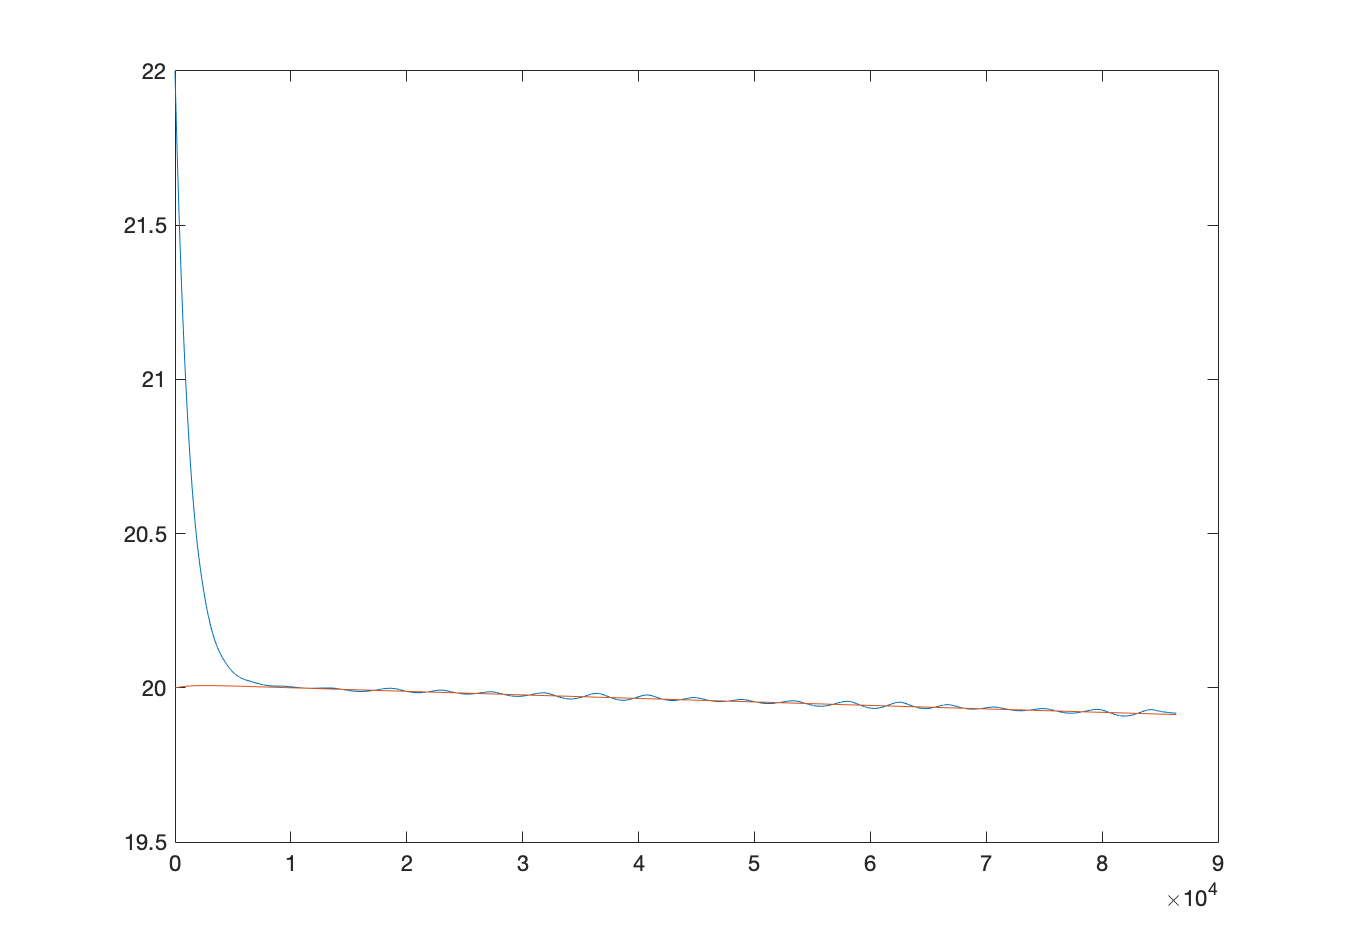
\includegraphics[width=1\textwidth]{figures/1-2-1.png}
    \subcaption{1天内自然降温曲线}
    \label{fig:my_label}
    \end{minipage}
    \begin{minipage}[c]{0.45\textwidth}
    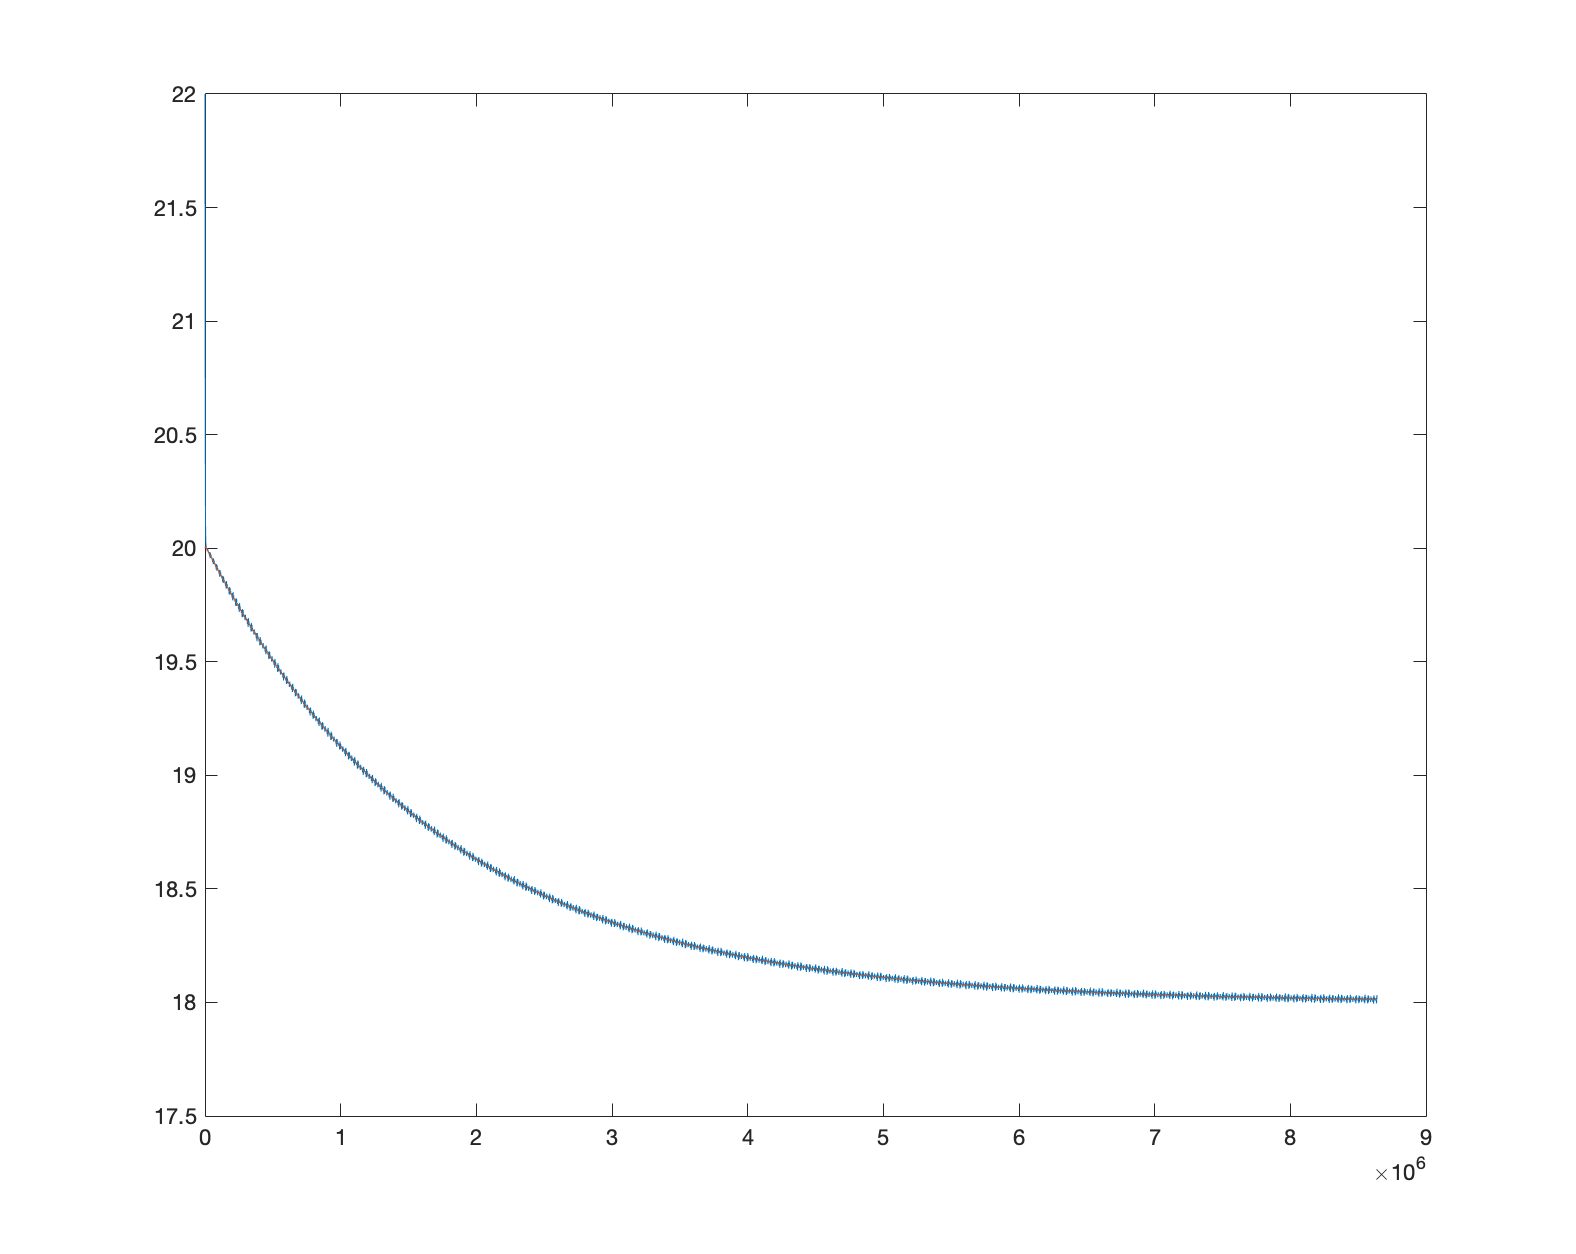
\includegraphics[width=.9\textwidth]{figures/1-2.png}
    \subcaption{100天自然降温曲线}
    \label{fig:my_label}
\end{minipage}
\caption{自然降温情况}
\end{figure}
\begin{example}
    \label{exa:example}
当室内初始温度为18度,墙体初始温度为15度,室外温度为-20度时,不考虑温控区间,开启采暖设备。
\end{example}
开启设备后,温度将持续地升高,观察图像可以看到,室内温度开始时升温较快,在2小时左右升温至24度,此后趋于平缓;墙体温度近似于线性地变化。

修改室外温度为0度,其余不变,此时观察图像发现室内和墙体温度的增长速度都变快了,在1小时左右即可升温至24度。
\begin{figure}[h]
    \centering
    \begin{minipage}[c]{0.45\textwidth}
        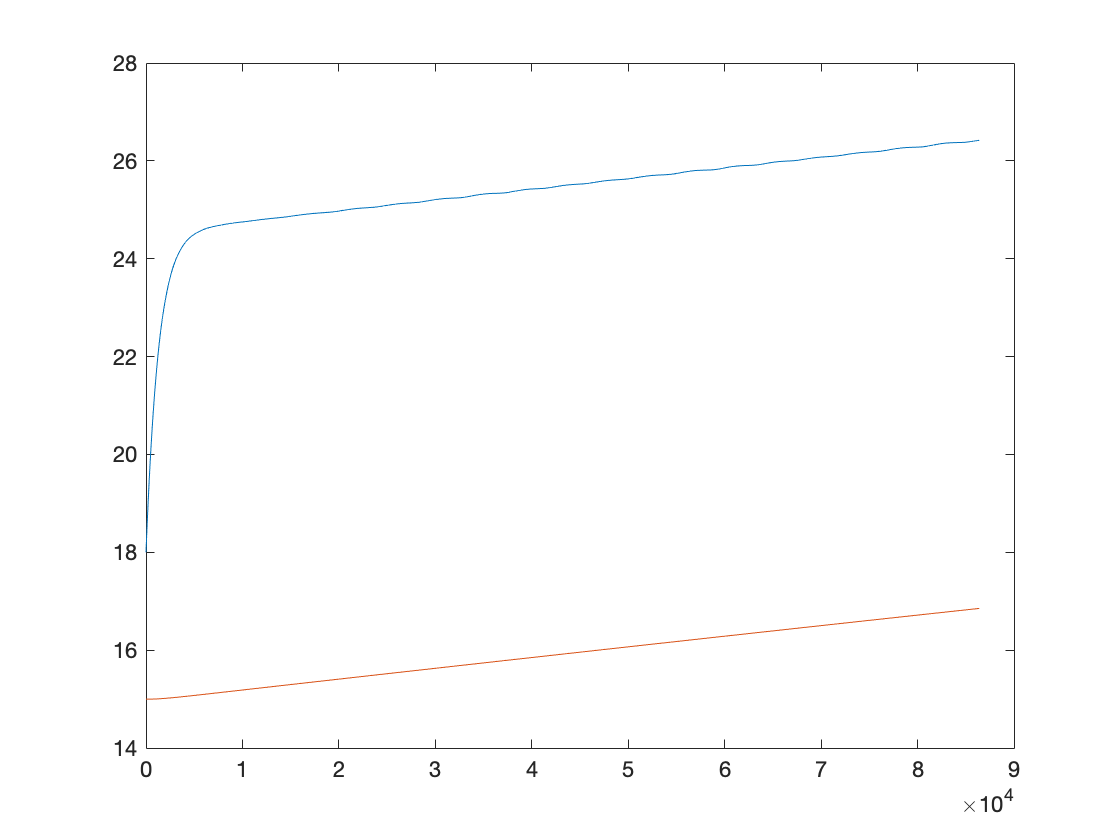
\includegraphics[width=1\textwidth]{figures/1-3-1.png}
    \subcaption{室外温度为-20度升温曲线}
    \label{fig:my_label}
    \end{minipage}
\begin{minipage}[c]{0.45\textwidth}
    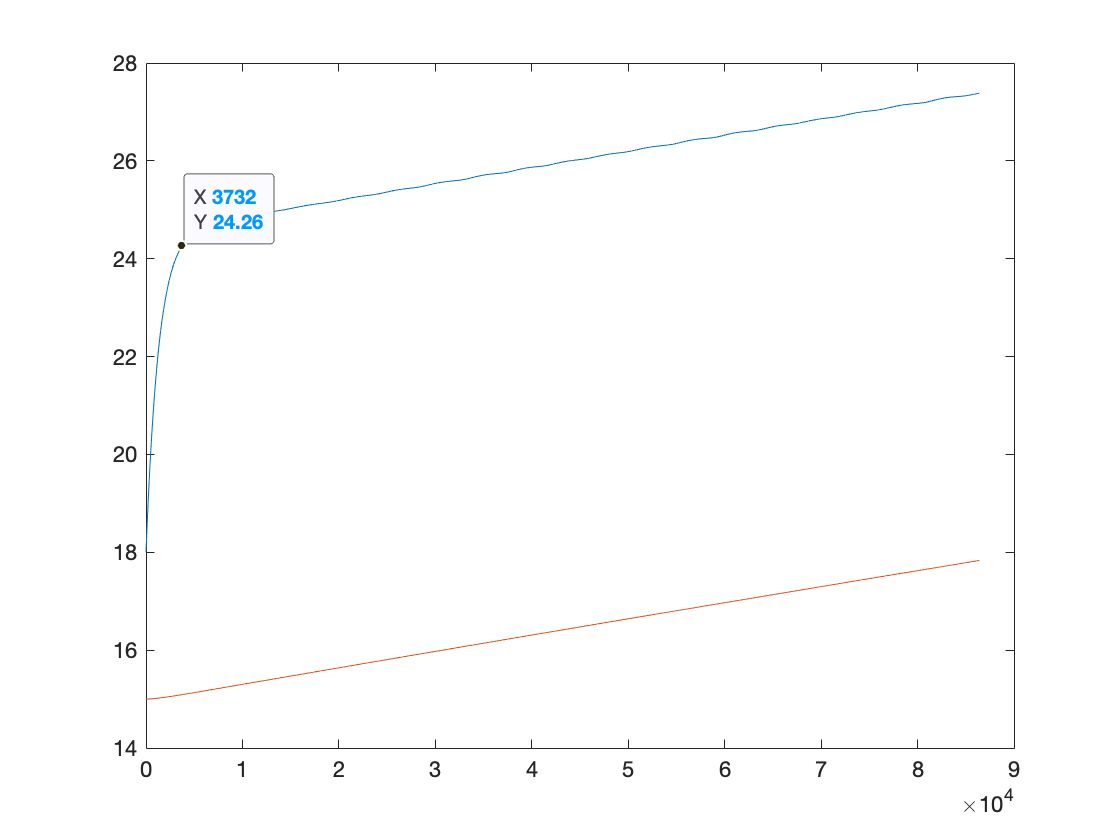
\includegraphics[width=1\textwidth]{figures/1-3-2.png}
    \subcaption{室外温度为0度升温曲线}
    \label{fig:my_label}
\end{minipage}
\caption{持续升温情况}
\end{figure}


\begin{example}
    \label{exa:example}
考虑温控区间,研究在室内温度18度时开启采暖设备,22度时关闭的周期性变化。
\end{example}
设室内初始温度为22度,此时关闭采暖设备,墙体初始温度为15度,室外初始温度为-20度。绘制温度的周期性变化图与电功率$P_{heat}(t)$大致如下图。

可以观察到,每次开启设备和关闭设备,所经历的时间是相似的,因此可以近似将一次降温一次升温过程视作一个周期,周期性的变化也可以视作是稳态。室内温度表现出规律性地升温降温,墙体温度一直趋于平稳,但是其实也有缓慢上升的趋势。

室外温度改为0度再次绘制曲线,周期变化趋势相似,但是根据例2的分析,此时室内升温将更快。
\begin{figure}[h]
    \centering
    \begin{minipage}[c]{0.45\textwidth}
        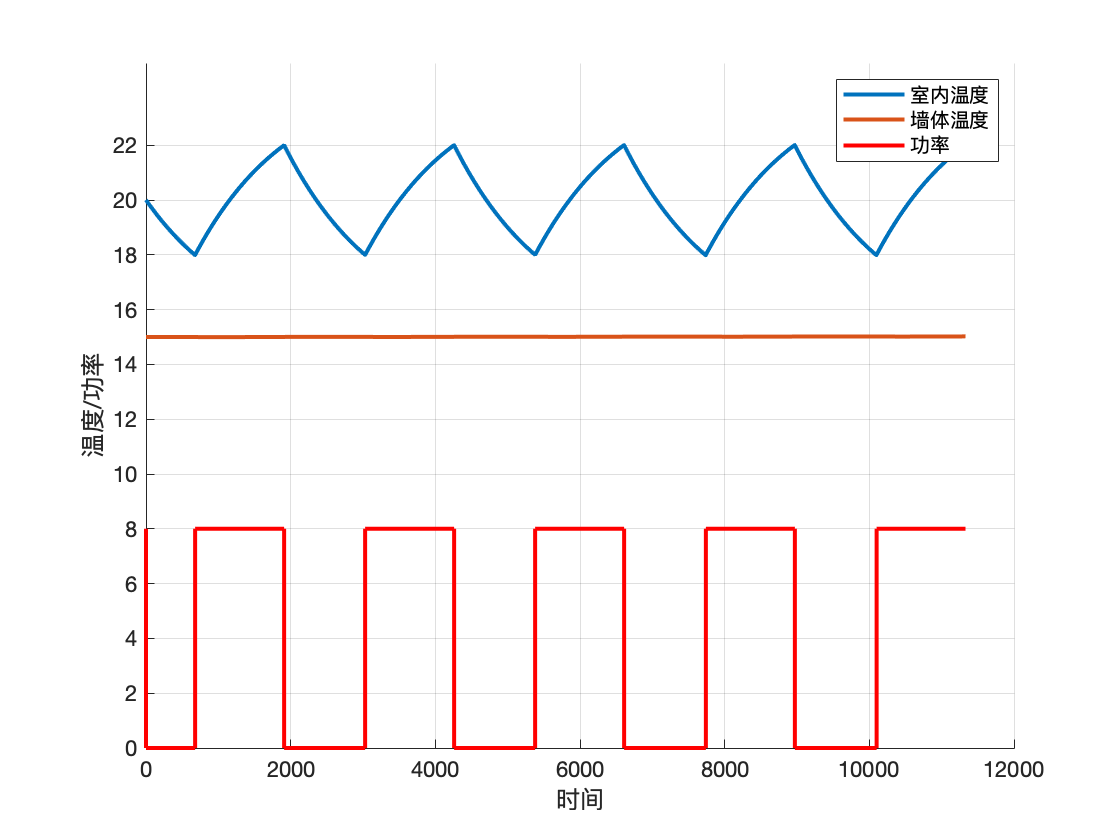
\includegraphics[width=1\textwidth]{figures/1-1-2.png}
    \subcaption{室外温度为-20度曲线}
    \label{fig:my_label}
    \end{minipage}
\begin{minipage}[c]{0.45\textwidth}
    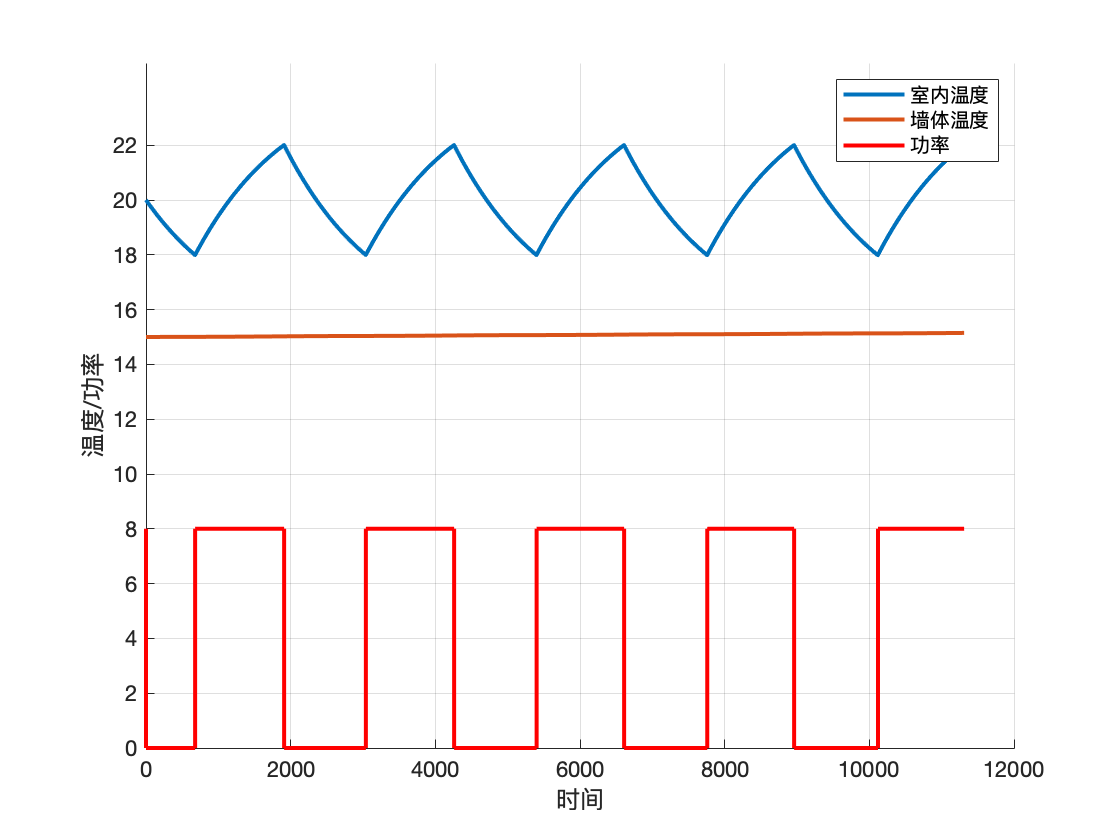
\includegraphics[width=1\textwidth]{figures/1-1-3.png}
    \subcaption{室外温度为0度曲线}
    \label{fig:my_label}
\end{minipage}
\caption{室外温度影响下的温度曲线}
\end{figure}

室内初始温度20度、室外温度-20度不变,改变墙体初始温度为13度和10度,分别绘制对应的曲线。

根据图像发现,墙体初始温度对曲线的变化影响更大,墙体温度为13度时,经过半天才能完成升温,墙体温度为10度时,室内温度降温更快,升温更慢,需要一天都开着采暖设备才能达到22度。
\begin{figure}[h]
    \centering
    \begin{minipage}[c]{0.45\textwidth}
        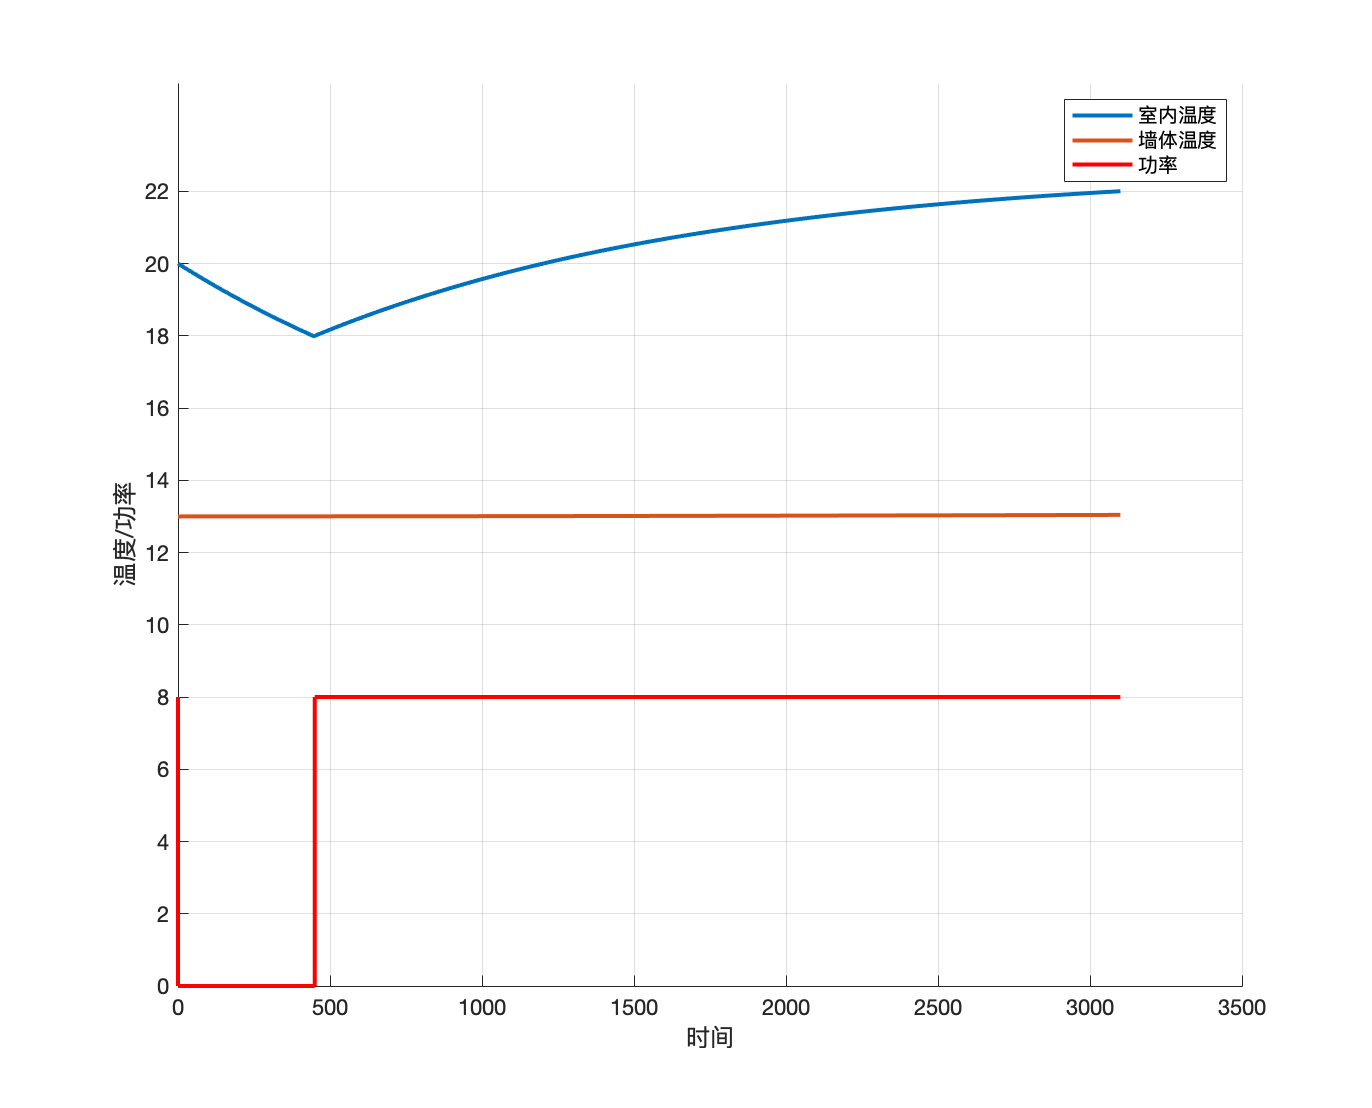
\includegraphics[width=1\textwidth]{figures/1-1-4.png}
    \subcaption{墙体初始温度为13度曲线}
    \label{fig:my_label}
    \end{minipage}
\begin{minipage}[c]{0.45\textwidth}
    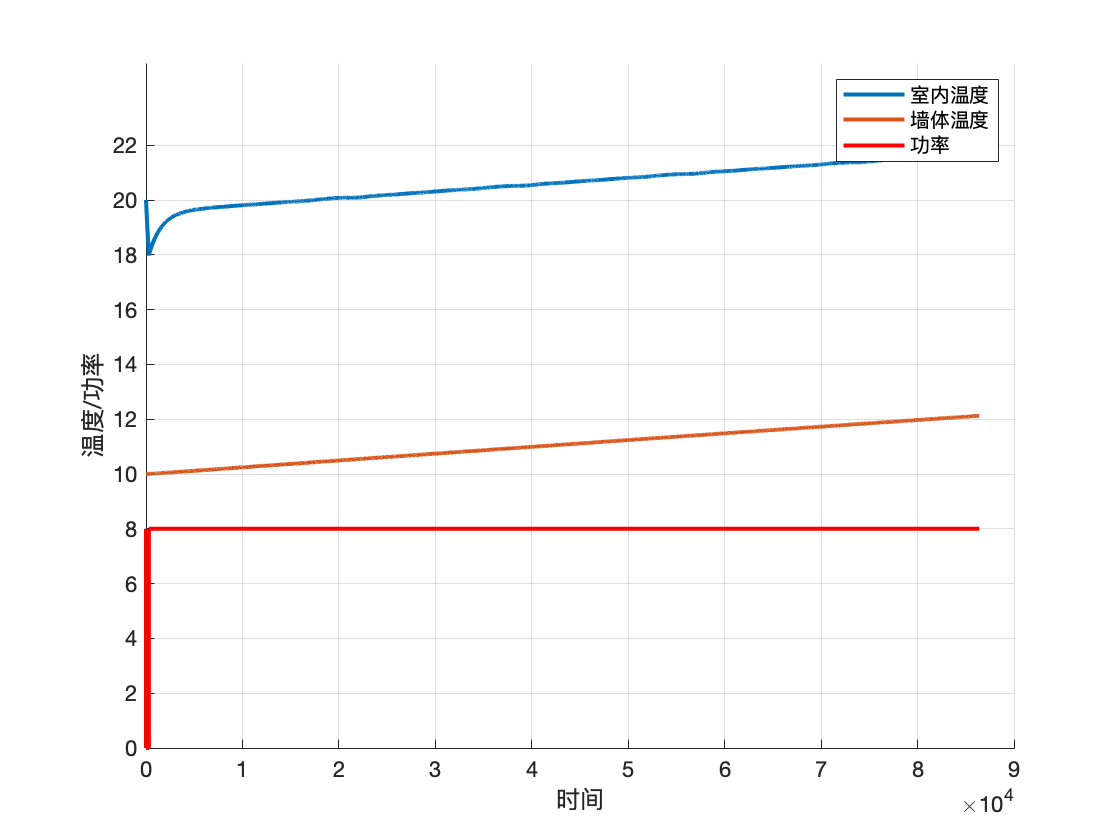
\includegraphics[width=1\textwidth]{figures/1-1-5.png}
    \subcaption{墙体初始温度为10度曲线}
    \label{fig:my_label}
\end{minipage}
\caption{墙体温度影响下的温度曲线}
\end{figure}

根据上文的分析,在温控区间内周期性变化时,室外温度、墙体初始温度都会对结果产生一定影响。室外温度对室内温度的影响较小,可以近似忽略,但墙体初始温度的影响较大。

墙体温度是一个比较复杂的变量,与室内外温度、墙的材质都有关,由于题目并没有给定墙体初始温度计算方法,在下文的研究中将根据已有的资料参考,自行决定较为合适的墙体温度。
\subsubsection{不同室外温度下典型住户电采暖用电行为统计}
在第二小问中,需要计算室外温度为-25到0度时,室内的平均升温、降温时长、用电量、电费等。在本小问的计算中,默认电采暖设备初始状态关闭。

通过软件计算,我们可以得到一天中的升温降温周期数量n,总升温、降温时长$t_1,t_2$。则平均升温降温时长计算方法为$\frac{t_1}{n},\frac{t_2}{n}$.平均占空比指的是通电时间占总时间的比例$\frac{t_1}{t_{total}}$,${t_{total}}=24\times 60\times 60=86400s=t_1+t_2$.日用电量为$t_1P_N$,即电采暖设备功率乘以升温时间。0-8时、21到24时为谷时,电价0.32,8-21时为峰时,电价0.56.由于题目中未规定t=0时,初始时间为一天中的几点,且采暖设备周期性分布比较规律,这里采用平均的方法来计算电价,平均电价为:$(11\times 0.32 + 13\times 0.56)\div 24 = 0.45$.

墙体温度根据现实生活中的经验,与室内温度有5度左右差距,假设房间条件较为恒温,墙体隔热效果较好,室外温度的综合影响较小,墙体初始温度分别定为15,14.6,14.2,13.8,13.4,13度。
\begin{table}
		\centering
		\caption{典型住户电采暖负荷用电行为特征量统计结果(室内初始温度为20度)}
	\resizebox{\linewidth}{!}{
	\begin{tabular}{|p{1.25cm}|p{1.5cm}|p{1.25cm}|p{1.25cm}|p{1.25cm}|p{1.25cm}|p{1.25cm}|p{1.25cm}|}\hline

	室外温度	&平均升温时长/min	&平均降温时长/min	&周期/min	&平均占空比/\%	&日用电量/kWh	&日平均用电功率/kW & 日用电成本/元 \\ \hline
	0 $^\circ$C &17.89	&  21.32	&39.22 &	45.62 &  88.29 & 3.64  & 39.73\\ \hline
	-5 $^\circ$C &20.500& 19.500& 40.00& 52.2 & 100.22 &  4.17& 45.100  \\ \hline
	  -10 $^\circ$C&22.5833 & 17.2222 & 39.8 & 56.73 &108.4 & 4.5387 &48.78 \\ \hline
-15 $^\circ$C& 25.2857&15.8571 &41.1429 &61.46 &118 & 4.9167 &53.1\\ \hline
 -20 $^\circ$C&28.944 & 14.6919 & 43.6364&66.33 & 127.355& 5.3065 &57.31\\ \hline
 -25 $^\circ$C& 35.689 &  13.621 & 49.65& 72.32 &138 & 5.7856 &62.100\\ \hline
	\end{tabular}
}
\end{table}
\begin{table}
		\centering
		\caption{周期性统计}
\begin{tabular}{|c|c|c|c|}\hline
	温度 &总升温时长/min& 总降温时长/min &近似周期个数 \\ \hline
0 $^\circ$C &662.1667 & 789.3333 & 37 \\ \hline
-5 $^\circ$C & 688.3333& 751.6667& 36\\ \hline
  -10$^\circ$C &813 & 620 &36\\ \hline
   -15$^\circ$C &885 & 555 & 35 \\ \hline
   -20$^\circ$C & 955.1667&484.833 &33\\ \hline
    -25 $^\circ$C &1035 & 395 &29\\ \hline
\end{tabular}
\end{table}

绘制出一日24h的室内温度变化和相应的电采暖设备开关状态曲线如下图所示。
\begin{figure}[H]
    \centering
    \begin{minipage}[c]{0.49\textwidth}
        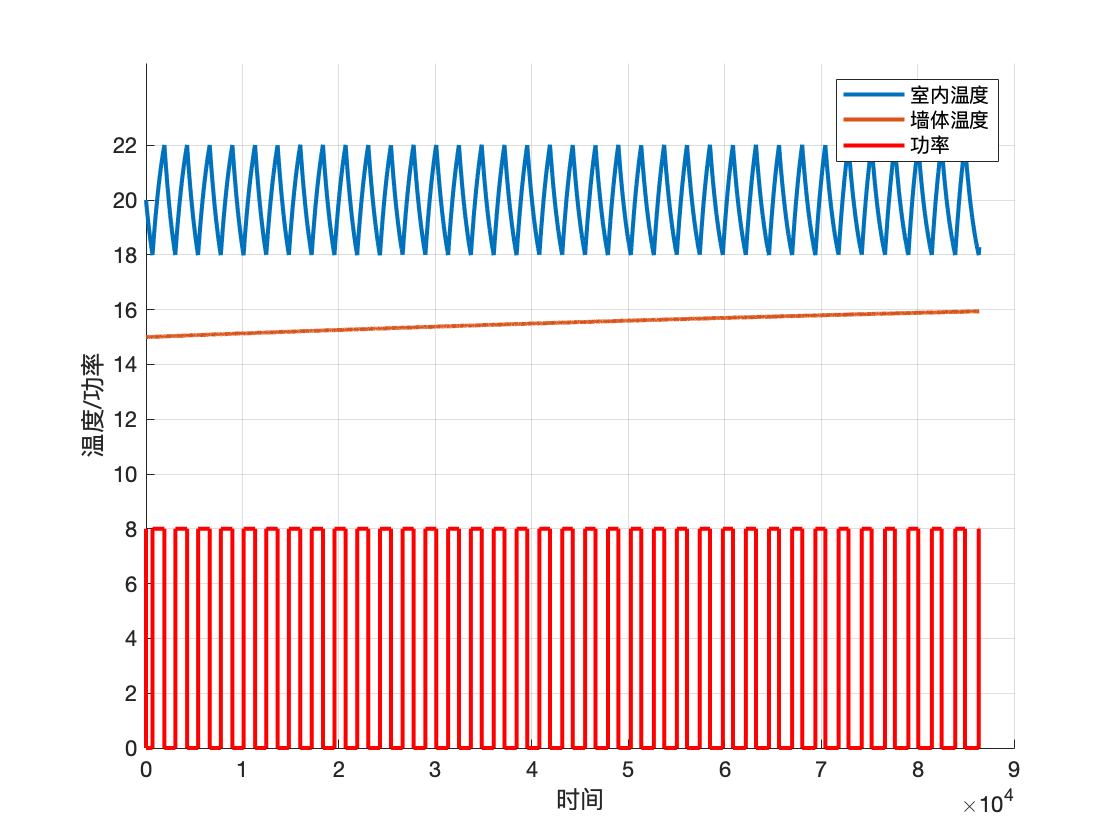
\includegraphics[width=1\textwidth]{figures/1-20-15.png}
    \subcaption{初始室温20度,墙体15度,室外0度}
    \label{fig:my_label}
    \end{minipage}
\begin{minipage}[c]{0.49\textwidth}
    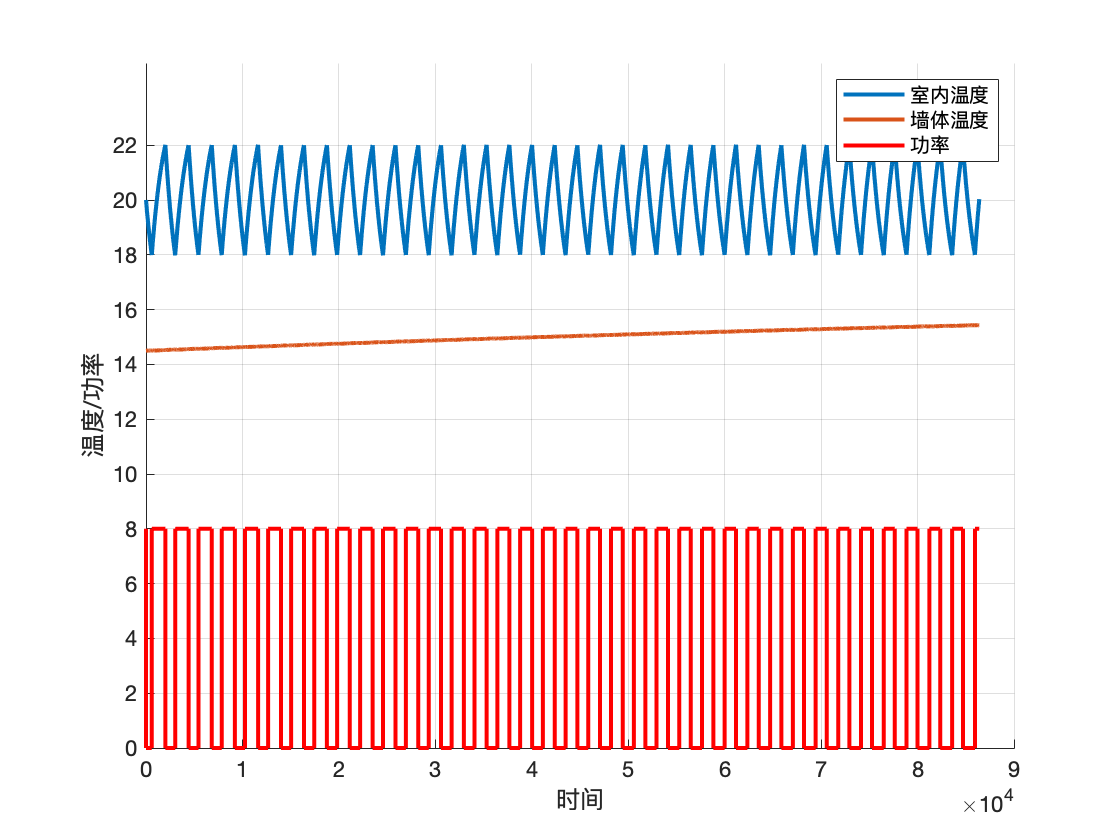
\includegraphics[width=1\textwidth]{figures/1-20-15-5.png}
    \subcaption{初始室温20度,墙体14.6度,室外-5度}
    \label{fig:my_label}
\end{minipage}
\begin{minipage}[c]{0.49\textwidth}
    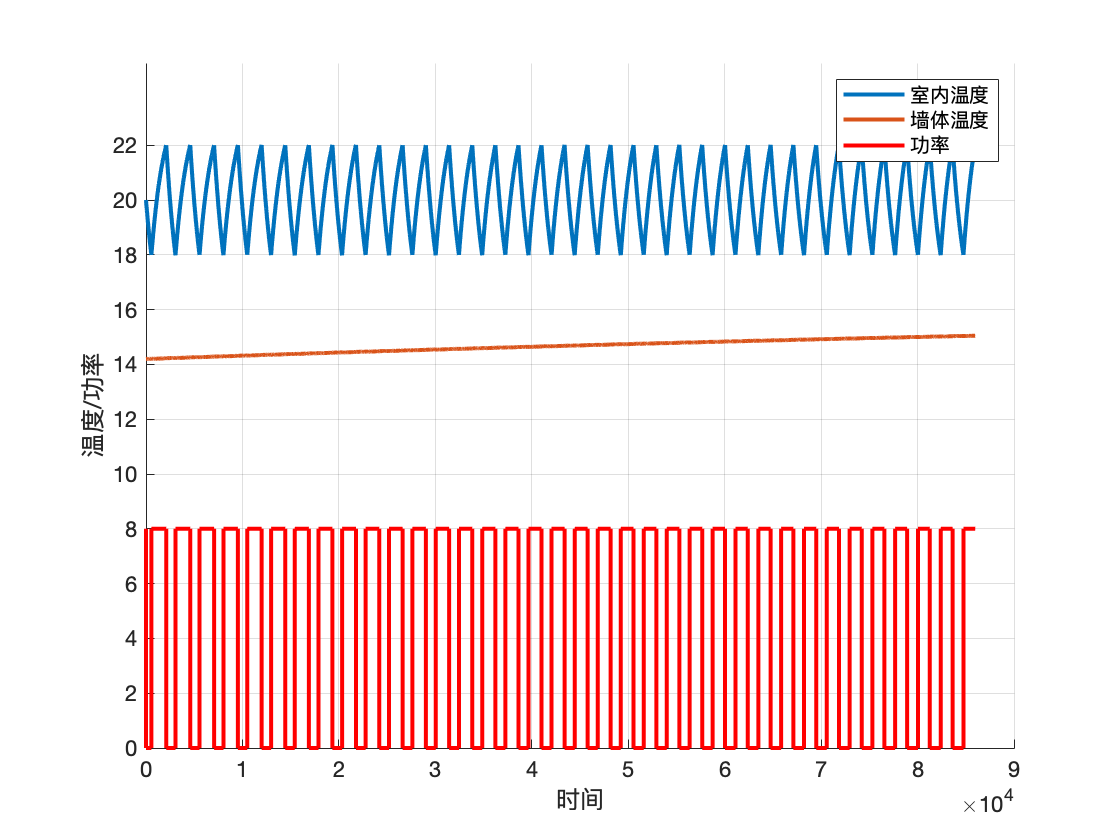
\includegraphics[width=1\textwidth]{figures/1-20-15-10.png}
    \subcaption{初始室温20度,墙体14.2度,室外-10度}
    \label{fig:my_label}
\end{minipage}
\begin{minipage}[c]{0.49\textwidth}
    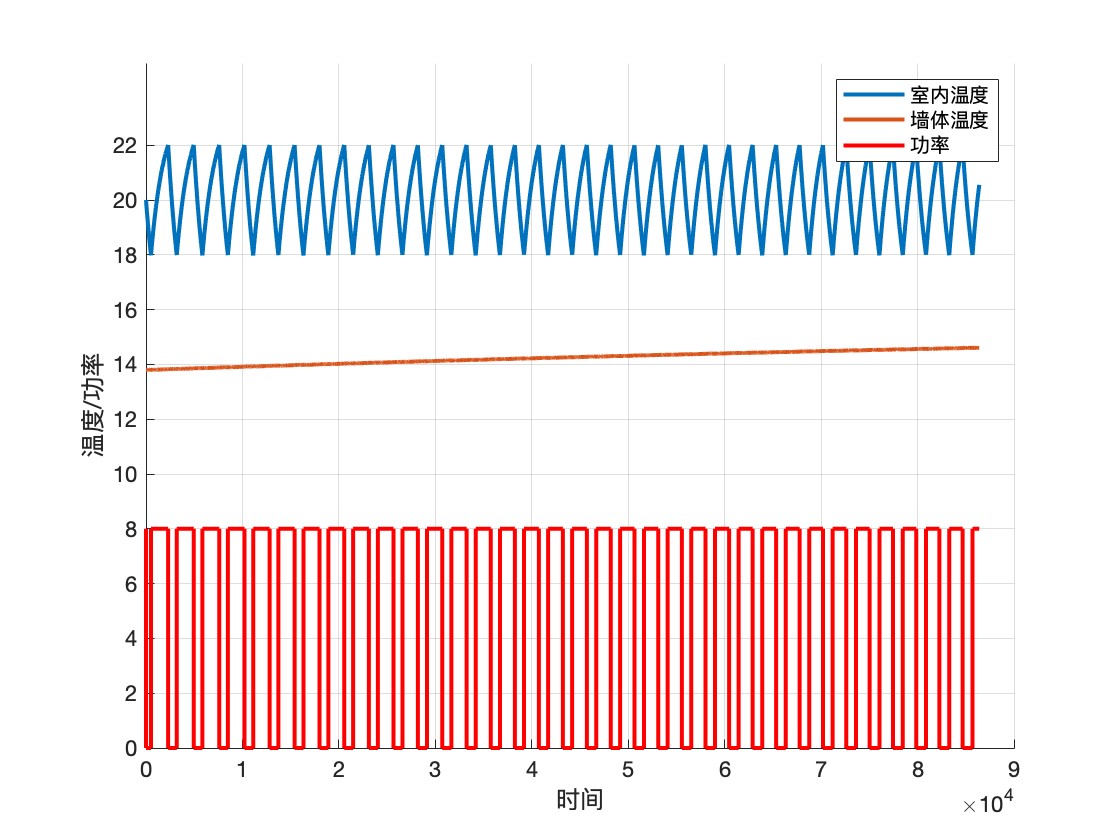
\includegraphics[width=1\textwidth]{figures/1-20-15-15.png}
    \subcaption{初始室温20度,墙体13.8度,室外-15度}
    \label{fig:my_label}
\end{minipage}
\begin{minipage}[c]{0.49\textwidth}
    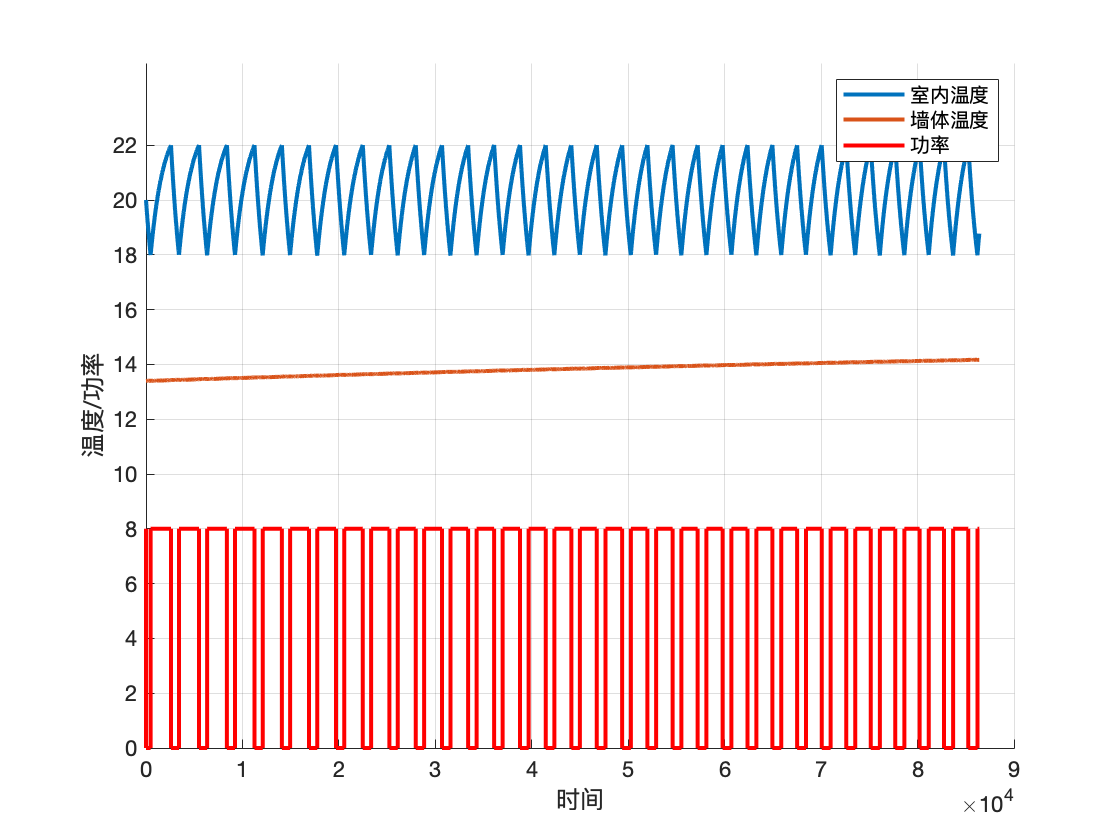
\includegraphics[width=1\textwidth]{figures/1-20-15-20.png}
    \subcaption{初始室温20度,墙体13.4度,室外-20度}
    \label{fig:my_label}
\end{minipage}
\begin{minipage}[c]{0.49\textwidth}
    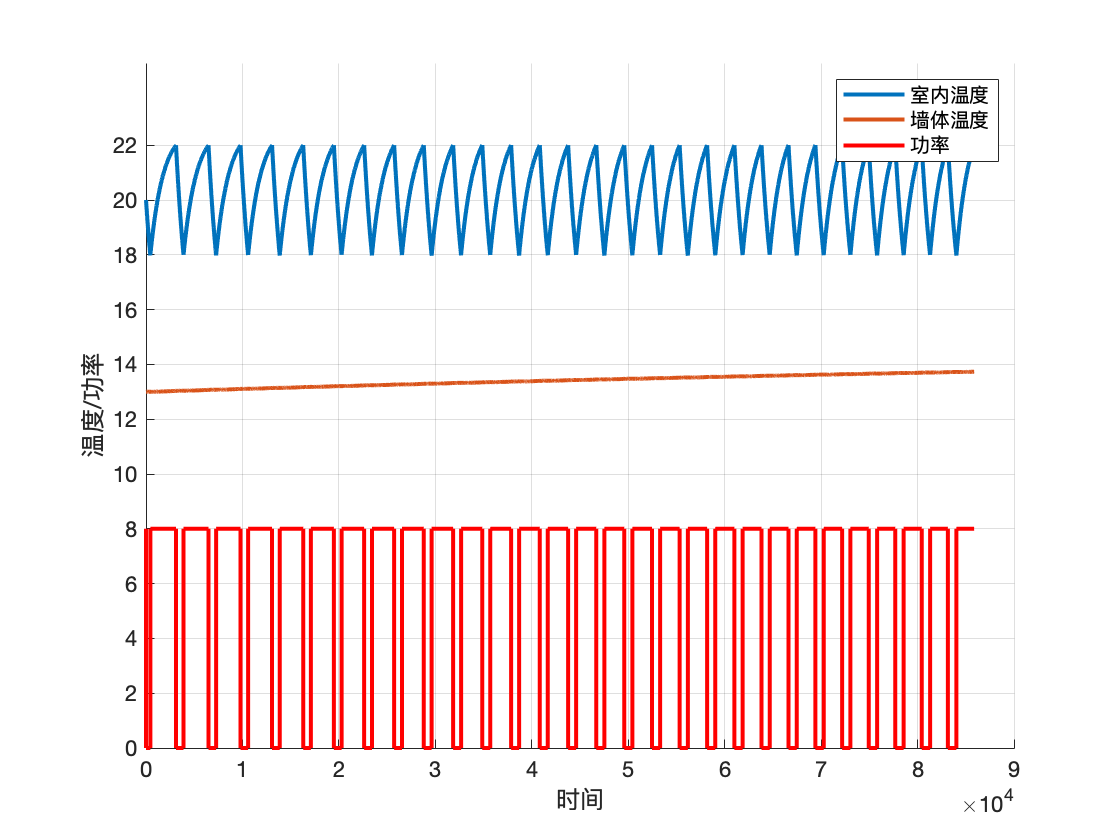
\includegraphics[width=1\textwidth]{figures/1-20-15-25.png}
    \subcaption{初始室温20度,墙体13度,室外-25度}
    \label{fig:my_label}
\end{minipage}
    \caption{不同温度对应室温初始20度的曲线}
\end{figure}
\subsubsection{供暖期内成本电量计算}
通过对上述结果的加和,可以得到总用电量和供暖成本的表格。
\begin{table}[H]
		\centering
		\caption{供暖期典型住户用电量和用电成本统计结果}
\begin{tabular}{|c|c|c|c|}\hline
室外平均温度 &持续天数& 用电量 & 供暖成本 \\ \hline
0 $^\circ$C &30 & 2648.7  & 1191.9 \\ \hline
-5 $^\circ$C & 40& 4008.8 & 1803.96\\ \hline
  -10$^\circ$C &40 & 4336 & 1951.2\\ \hline
   -15$^\circ$C &40 & 4720 & 2124 \\ \hline
   -20$^\circ$C & 40& 5094  & 2292.3\\ \hline
    -25 $^\circ$C & 30 &4140 & 1863\\ \hline
    总计&180 & 24947.5 & 11226.36\\ \hline
\end{tabular}
\end{table}
相对于实际情况,由于存在问题假设,计算得到的供暖成本可能高出许多。比如实际上功率并不能直接计算成额定功率,墙体的隔热性也有差别,这些因素的影响非常复杂。

\subsection{问题二\quad 典型住户电采暖负荷参与功率调节的能力分析}
\subsubsection{室外温度-15度时功率调节时间}
由题意,在电暖设备开启至温控区间上界22度时,为功率上调可持续时间;电暖设备关闭至温控区间下界18度时,为功率下调可持续时间。

以单个典型住户为对象进行分析,室内初始温度20度,室外温度为-15度,根据上一问的假设,墙体温度为13.8度,开关初始状态开启。此时以分钟为单位,绘制电暖设备的功率变化图.

\begin{figure}[h]
\centering
    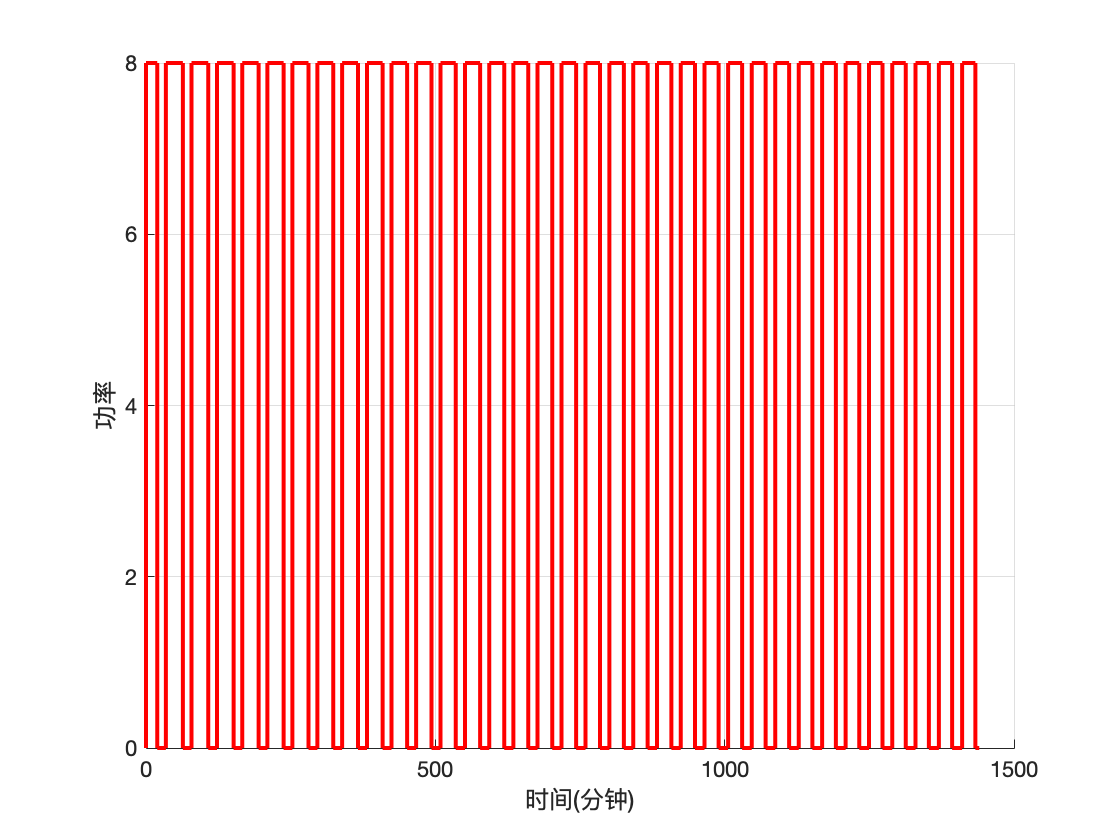
\includegraphics[width=0.7\textwidth]{figures/2-1-1.png}
    \caption{电暖设备功率变化图}
    \label{fig:my_label}
\end{figure}

设时间节点$t_k$开关开始打开,下一个最近的时间节点$t_{k+1}$开关关闭,温度上升至温控区间上界。再下一个最近时间节点$t_{k+2}$开关打开,温度下降到温控区间下界。则有:

 \[ t_{\mbox{上调}}= \left\{
  \begin{array}{rl}
t_{k+1}-t & t_k< t <t_{k+1},\\
 0 & t_{k+1}\leq  t \leq t_{k+2} .
 \end{array} \right. \]
 
  \[ t_{\mbox{下调}}= \left\{
  \begin{array}{rl}
0 & t_k< t <t_{k+1},\\
 t_{k+2}-t & t_{k+1}\leq  t \leq t_{k+2} .
 \end{array} \right. \]

根据上述结论,我们可以绘制出可参与功率调节的时间曲线。
\begin{figure}[H]
    \centering
    \begin{minipage}[c]{0.49\textwidth}
        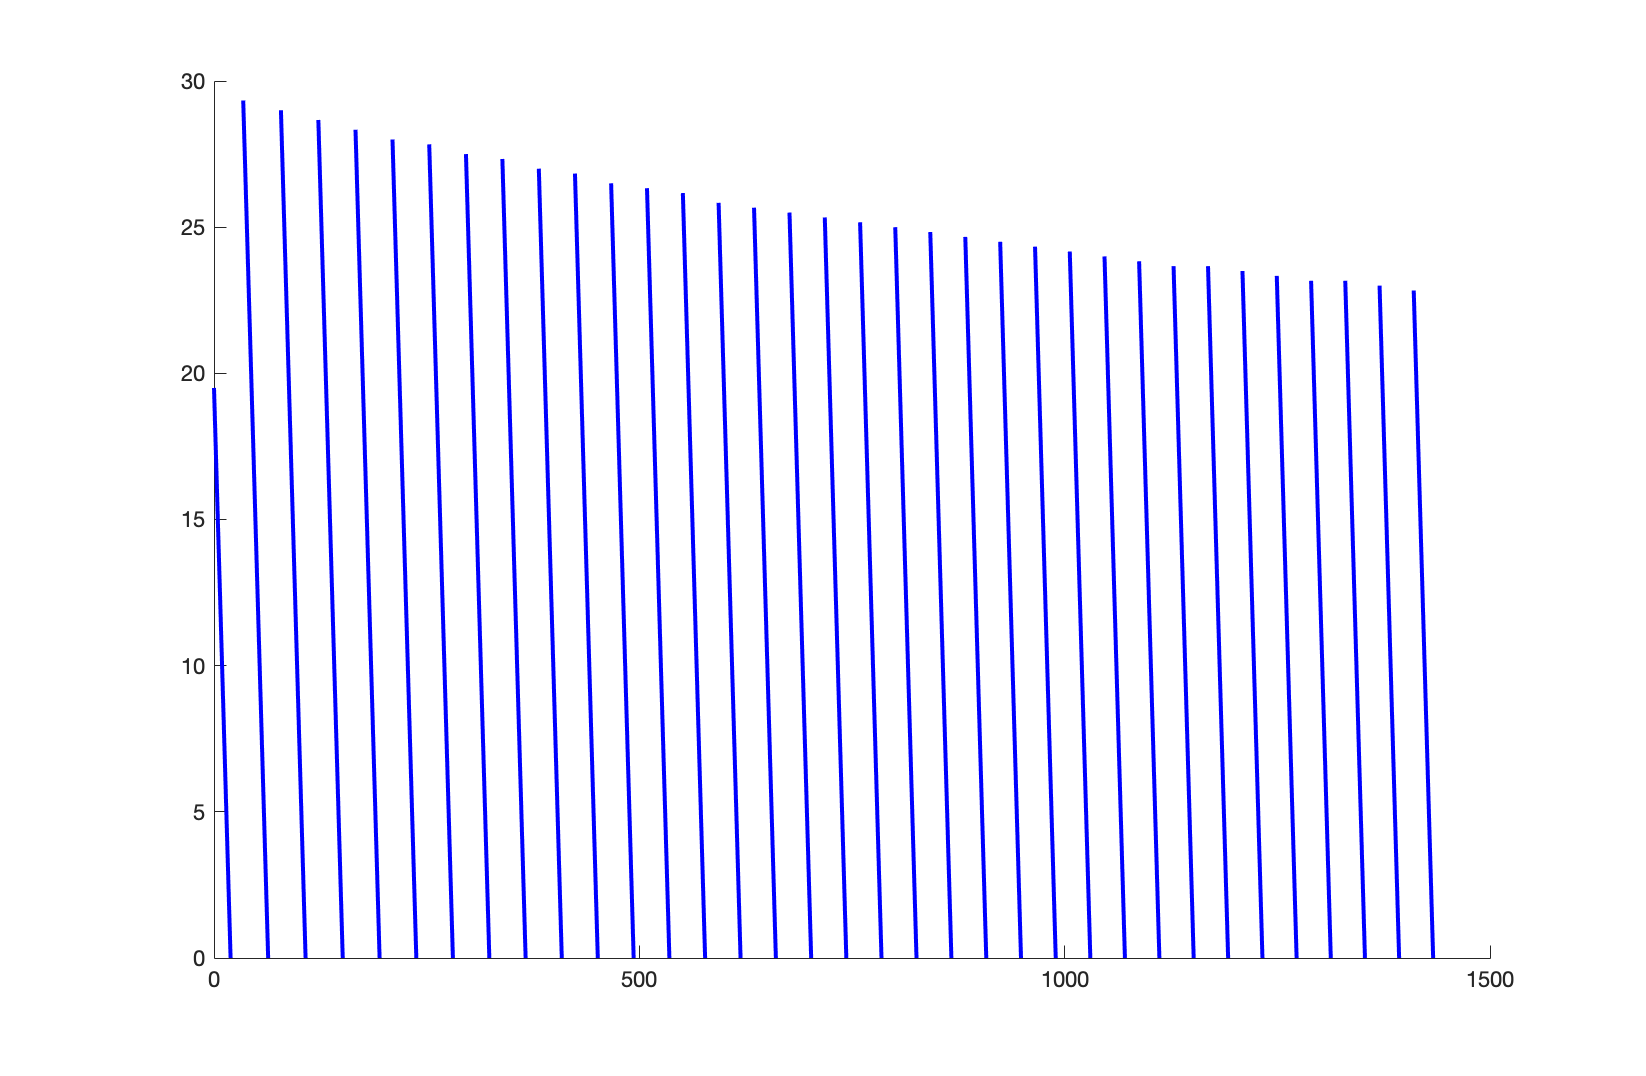
\includegraphics[width=1\textwidth]{figures/2-1-up.png}
    \subcaption{室外-15度可上调时间曲线(连续)}
    \label{fig:my_label}
    \end{minipage}
\begin{minipage}[c]{0.45\textwidth}
    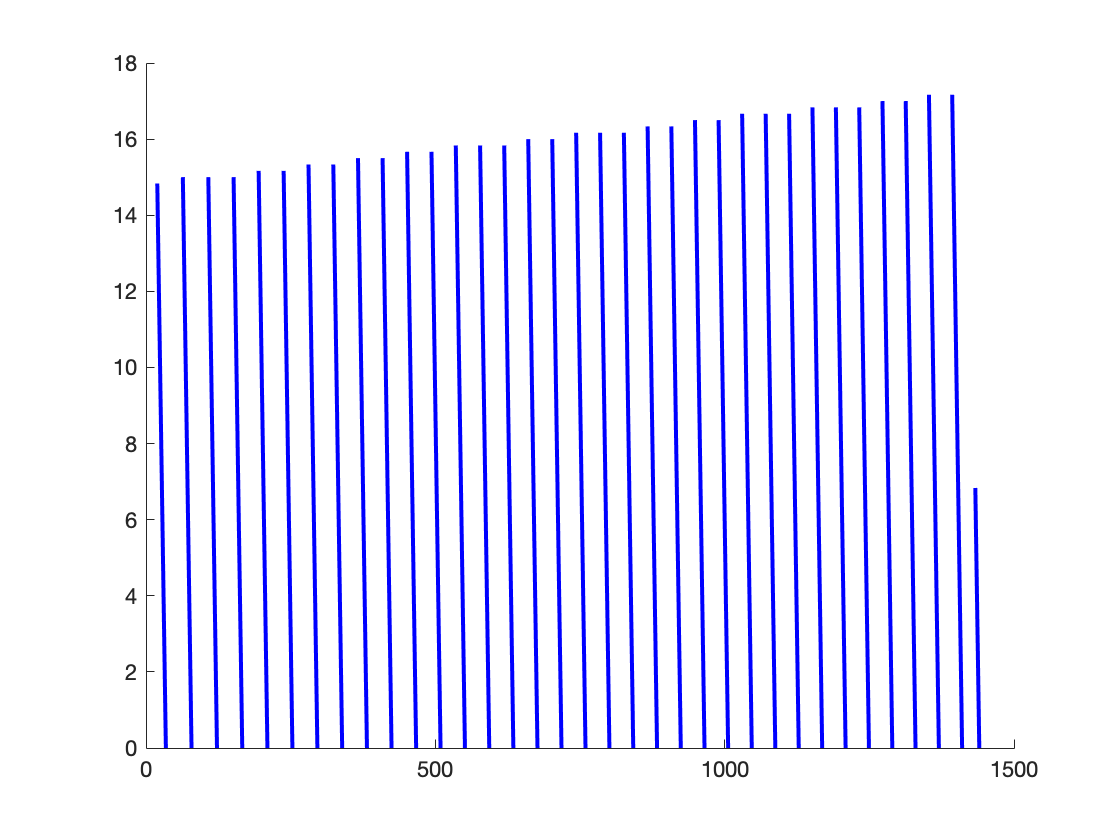
\includegraphics[width=1\textwidth]{figures/2-1-down.png}
    \subcaption{室外-15度可下调时间曲线(连续)}
    \label{fig:my_label}
\end{minipage}
\end{figure}

在本小问假设中,t代表了每个分钟时间点,只能取整数。$0\leq t \leq 1440$.这样计算出来的结果应该是离散的,在连续情况下,其上界可以构成光滑曲线,离散情况下构成的曲线比较凹凸不平。

绘制的以分钟为节点的图像如下图所示。
\begin{figure}[H]
    \centering
        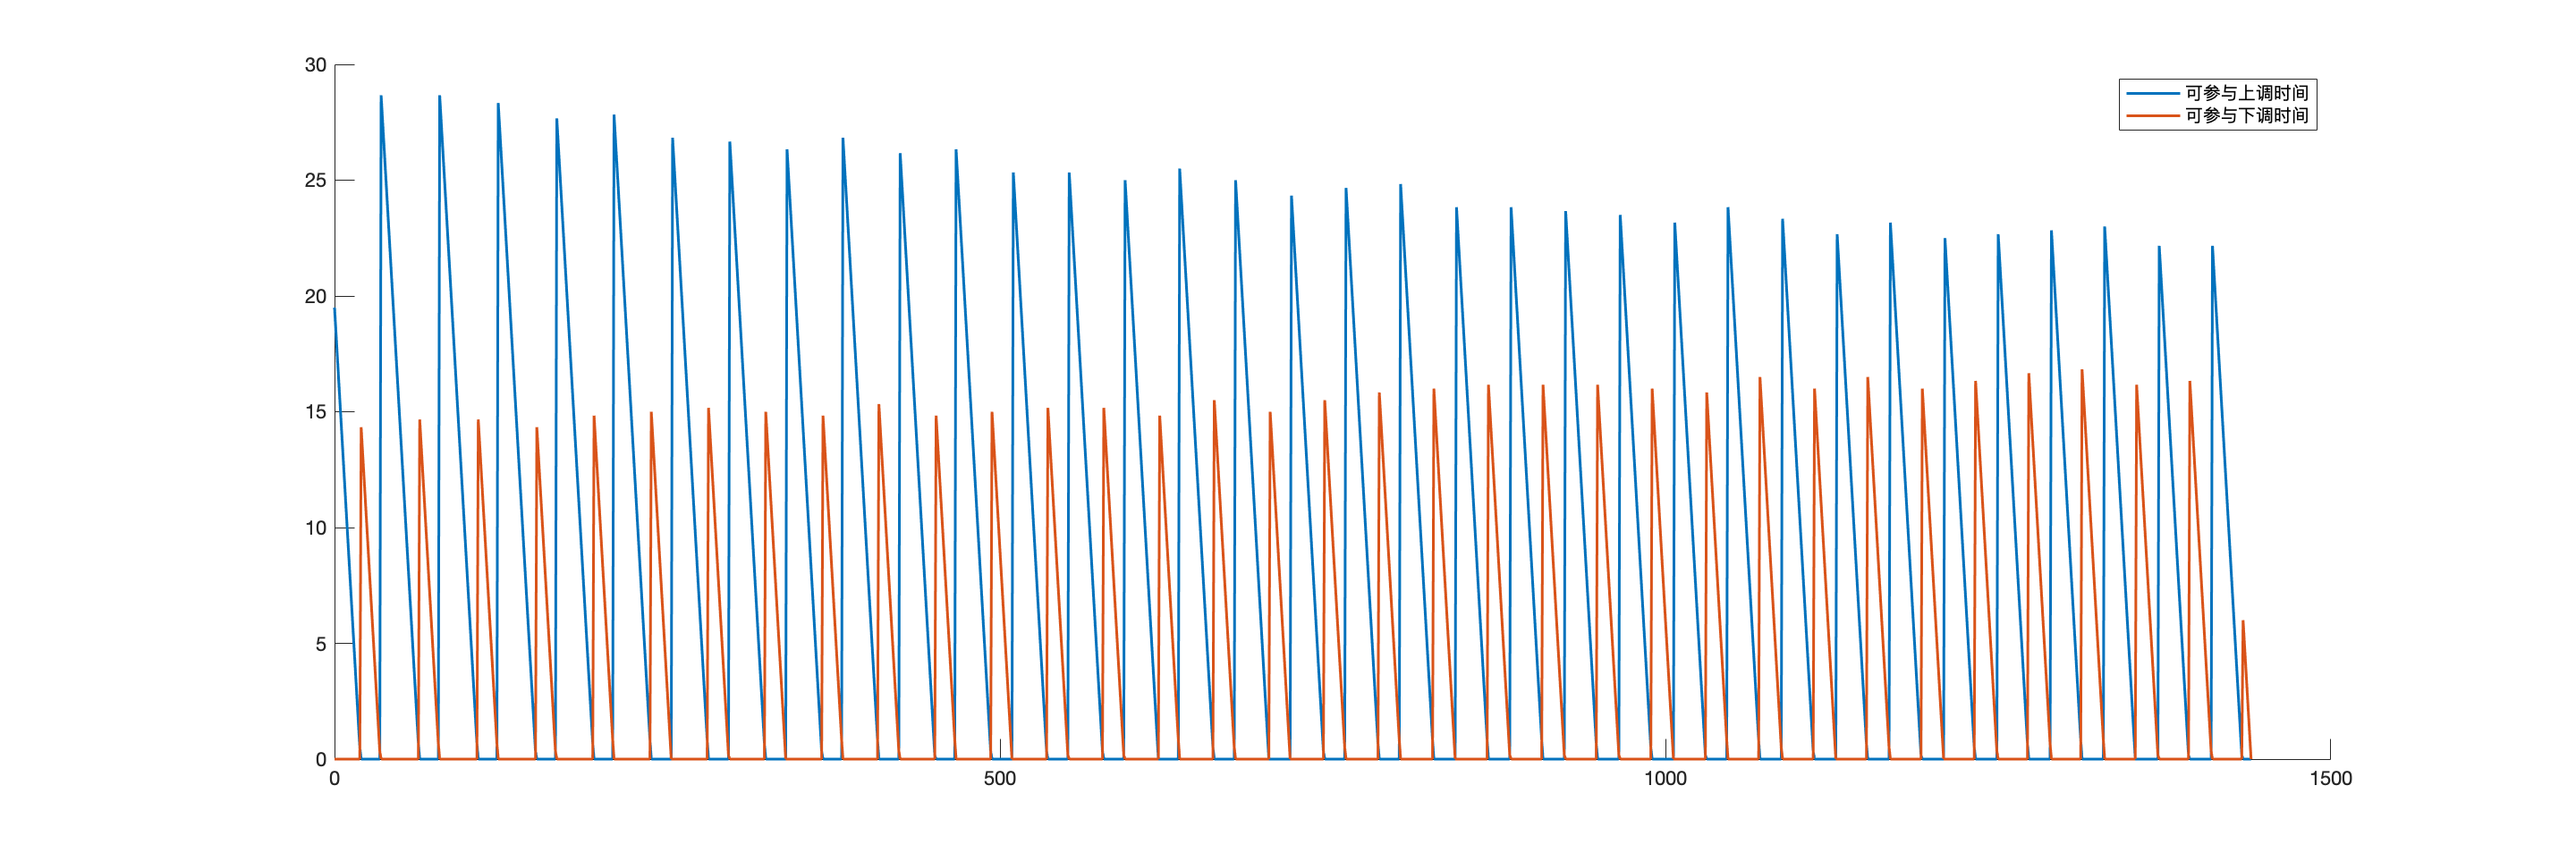
\includegraphics[width=1\textwidth]{figures/2-1minute.png}
    \caption{室外-15度可参与调节功率的时间曲线(分钟)}
    \label{fig:my_label}
    \end{figure}
由于正文篇幅有限,计算结果不能一一列举,这里举例列出了一部分计算得到的开启和关闭时间点,并以第一个周期为例给出了相应计算公式。
\begin{table}[H]
		\centering
\begin{tabular}{|c|c|}\hline
 开启时间点$t_{on}$ &关闭时间点$t_{off}$  \\ \hline
0	&19.50  \\ \hline
34.33 &	63.66  \\ \hline
78.66&	107.666\\ \hline
122.66 &	151.333 \\ \hline
166.333 &	194.6	 \\ \hline
	\end{tabular}
\end{table}
\begin{table}[H]
		\centering
\begin{tabular}{|c|c|c|}\hline
可上调时间 &可下调时间 & t取值  \\ \hline
19.50-t	& 0  & $ 0\leq t \leq 19$  \\ \hline
0 &	34.33-t  & $20\leq t \leq 34$  \\ \hline
	\end{tabular}
\end{table}
\subsubsection{不同室外温度的可调节功率时间曲线分析}
根据上一问表中的室外温度与墙体温度假设,保持室内初始温度为20度,电采暖设备开关的初始状态为开启,分别计算了功率可调节时间,并通过绘制曲线展示结果。

\begin{figure}[H]
    \centering
    \begin{minipage}[c]{0.35\textwidth}
        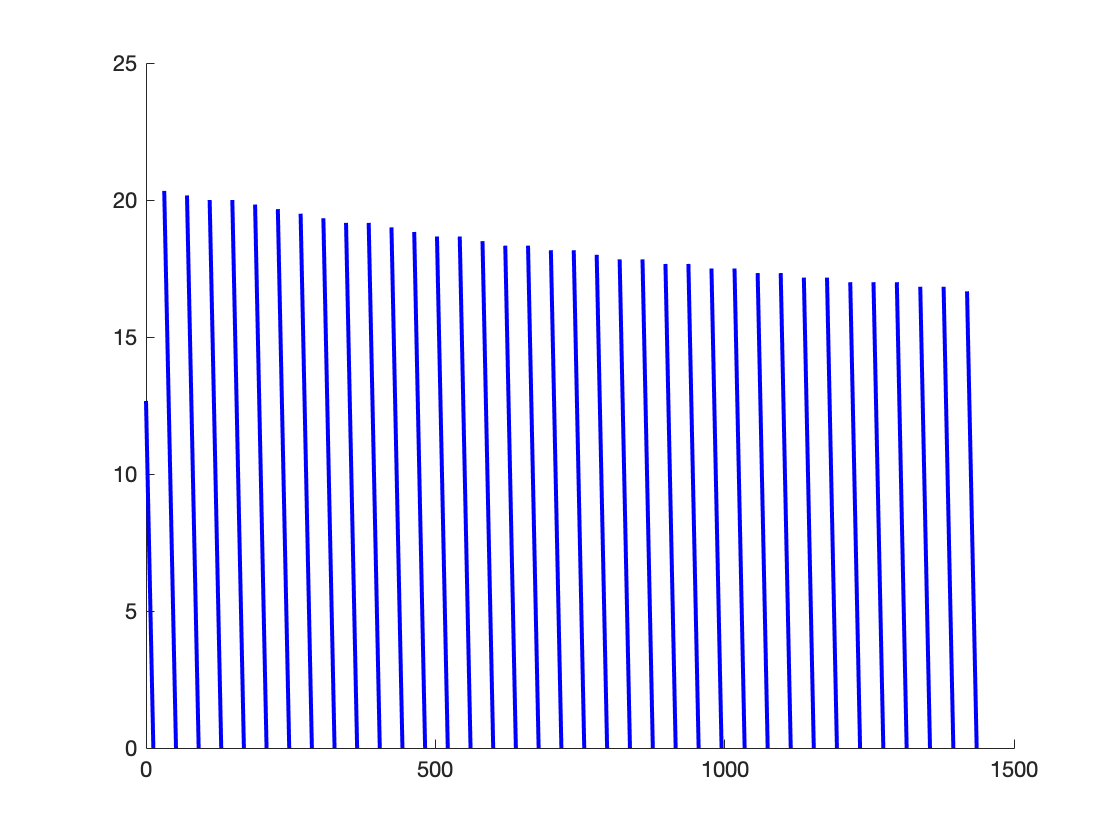
\includegraphics[width=1\textwidth]{figures/2-2-0-up.png}
    \subcaption{墙体15度,室外0度,可上调时间曲线}
    \label{fig:my_label}
    \end{minipage}
\begin{minipage}[c]{0.35\textwidth}
    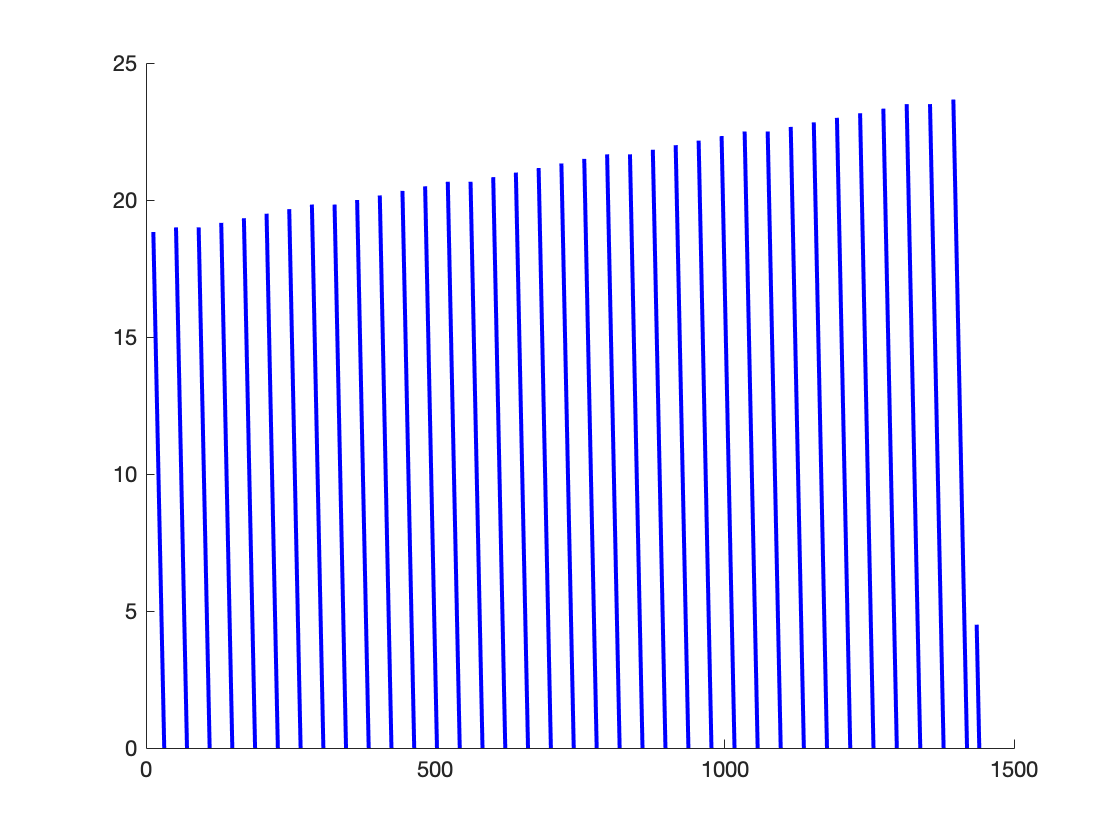
\includegraphics[width=1\textwidth]{figures/2-2-0-down.png}
    \subcaption{墙体15度,室外0度,可下调时间曲线}
    \label{fig:my_label}
\end{minipage}
 \begin{minipage}[c]{0.35\textwidth}
        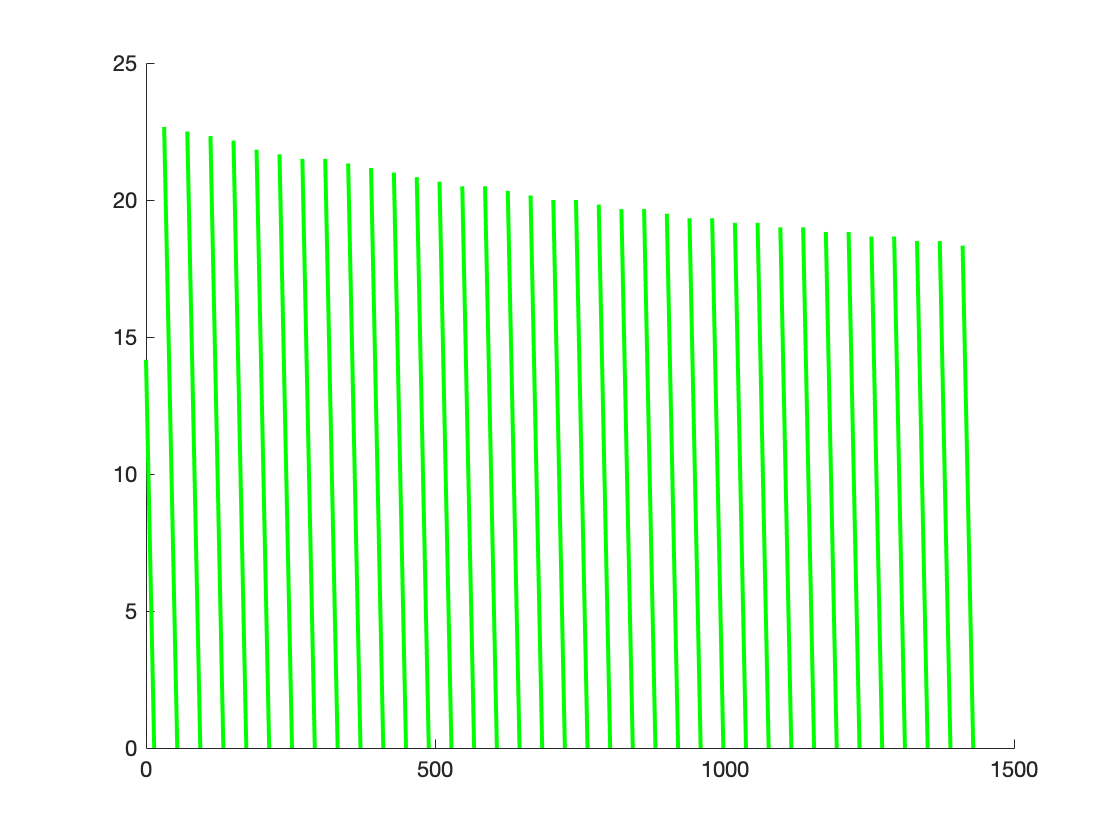
\includegraphics[width=1\textwidth]{figures/2-2-5-up.png}
    \subcaption{墙体14.6度,室外-5度,可上调时间曲线}
    \label{fig:my_label}
    \end{minipage}
\begin{minipage}[c]{0.35\textwidth}
    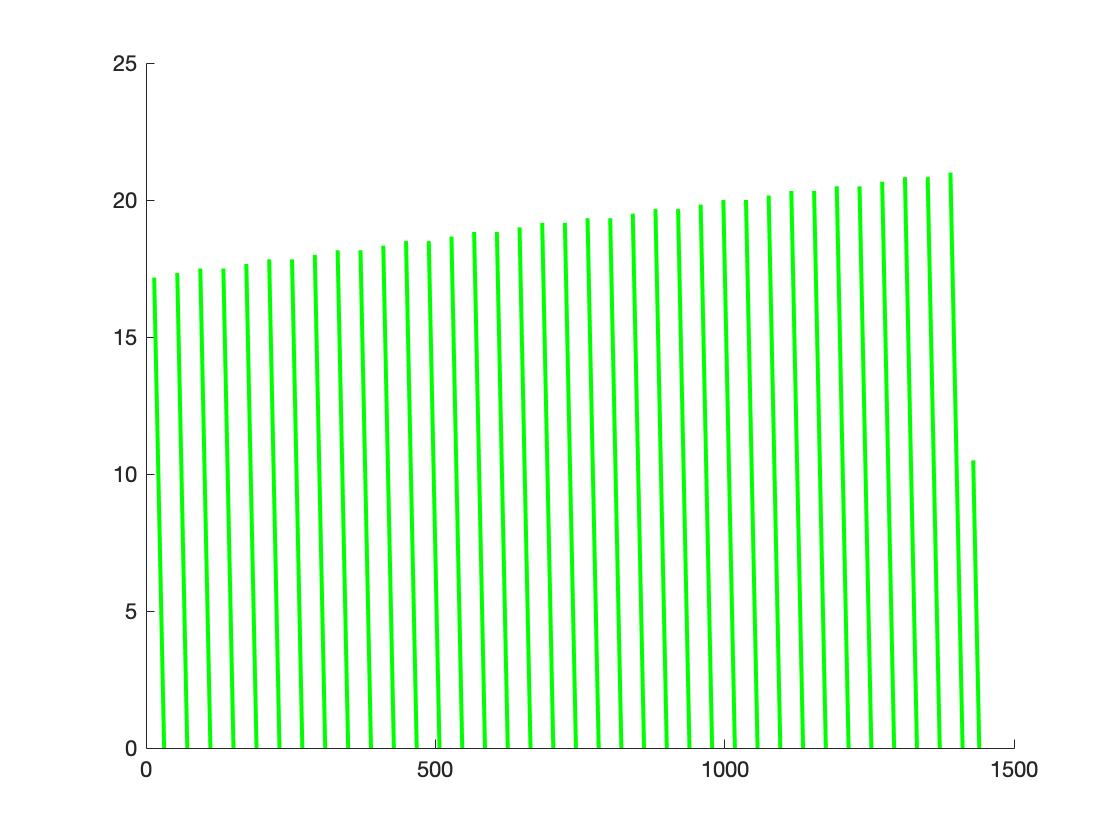
\includegraphics[width=1\textwidth]{figures/2-2-5-down.png}
    \subcaption{墙体14.6度,室外-5度,可下调时间曲线}
    \label{fig:my_label}
      \end{minipage}
     \begin{minipage}[c]{0.35\textwidth}
        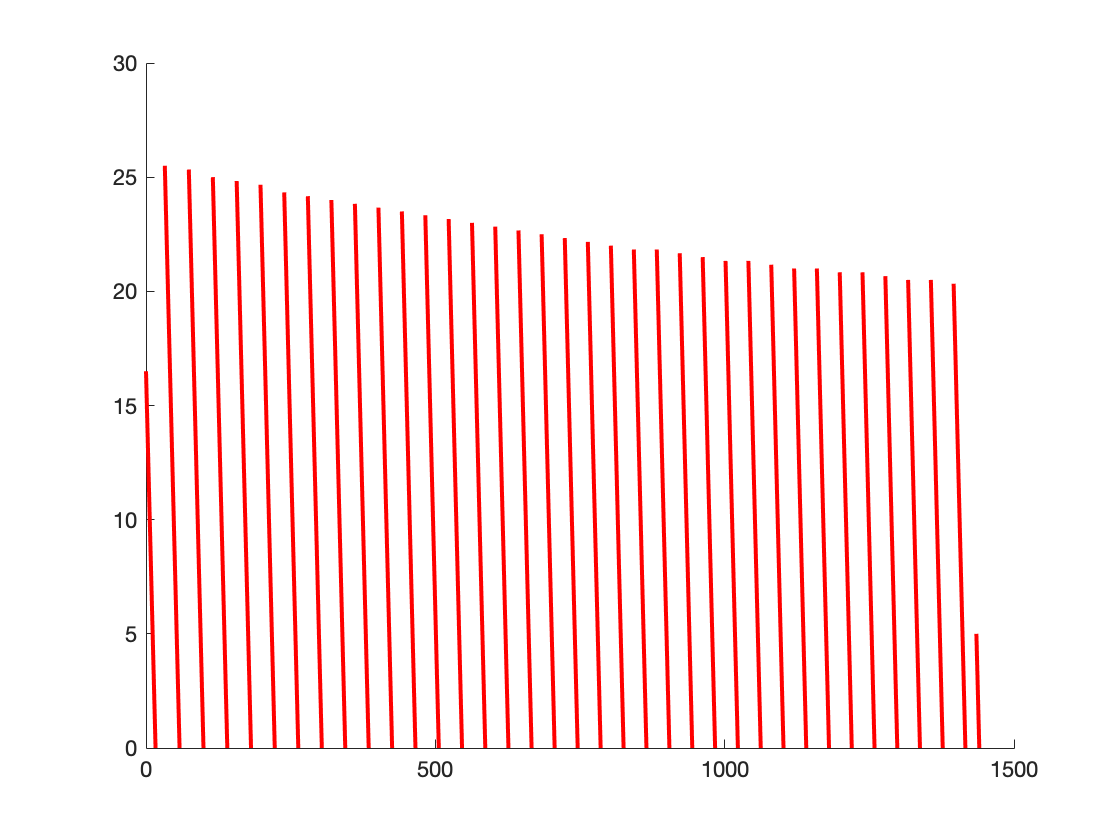
\includegraphics[width=1\textwidth]{figures/2-2-10-up.png}
    \subcaption{墙体14.2度,室外-10度,可上调时间曲线}
    \label{fig:my_label}
    \end{minipage}
\begin{minipage}[c]{0.35\textwidth}
    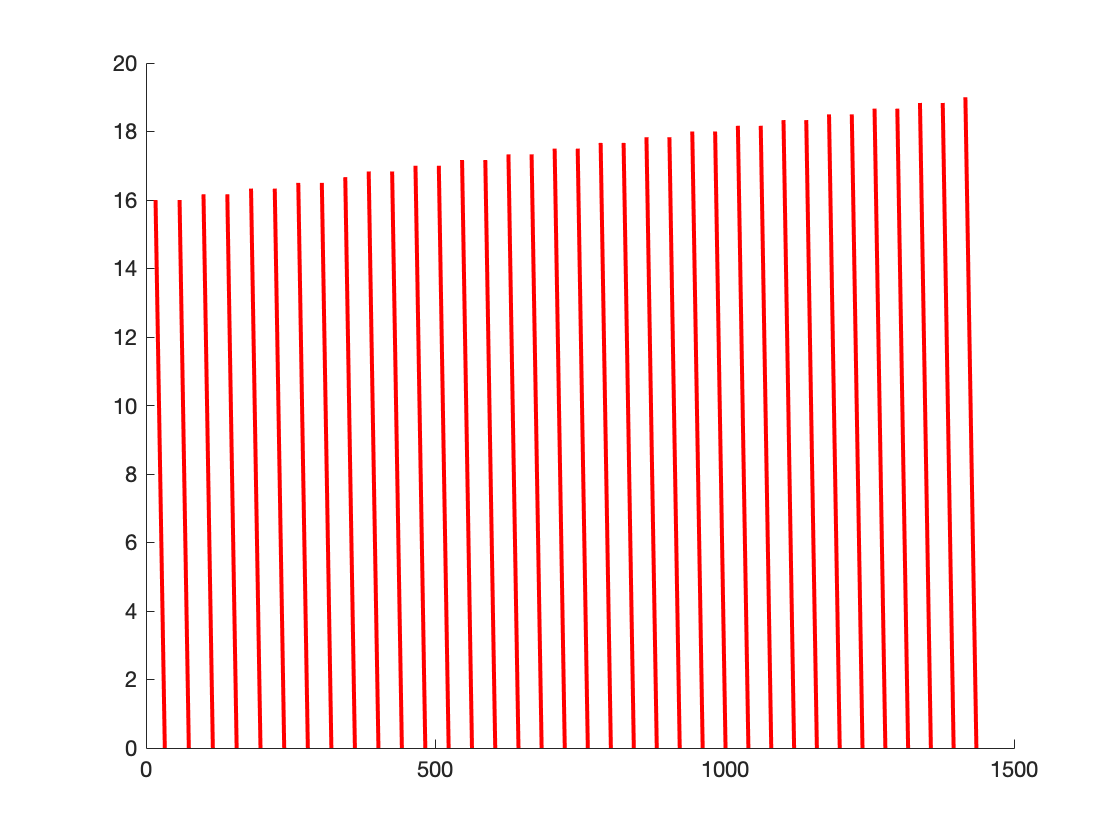
\includegraphics[width=1\textwidth]{figures/2-2-10-down.png}
    \subcaption{墙体14.2度,室外-10度,可下调时间曲线}
    \label{fig:my_label}
\end{minipage}
     \begin{minipage}[c]{0.35\textwidth}
        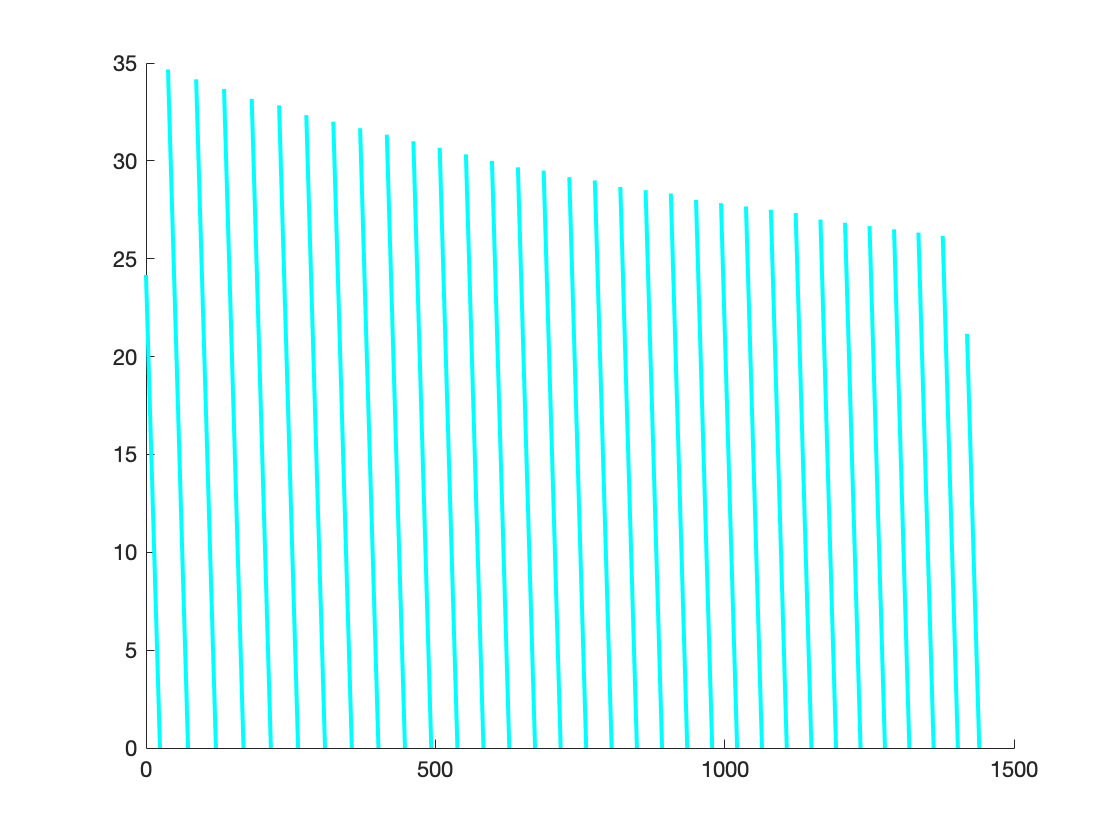
\includegraphics[width=1\textwidth]{figures/2-2-20-up.png}
    \subcaption{墙体13.4度,室外-20度,可上调时间曲线}
    \label{fig:my_label}
    \end{minipage}
\begin{minipage}[c]{0.35\textwidth}
    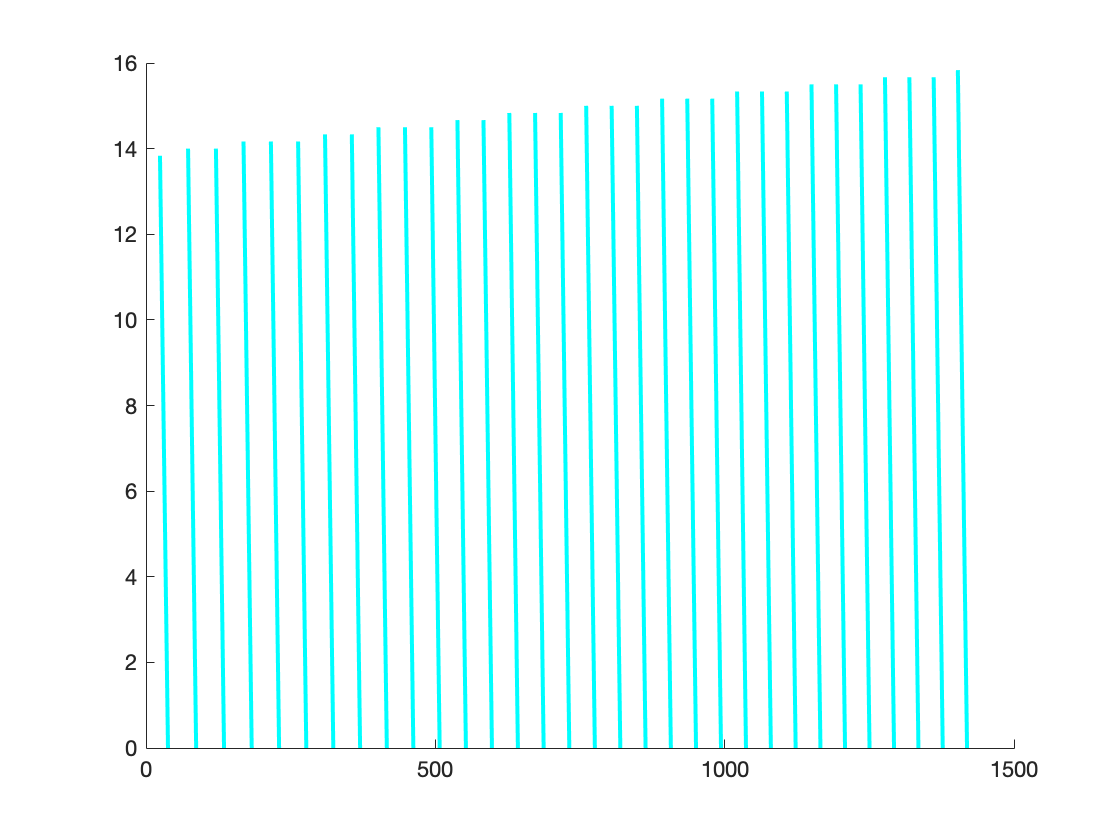
\includegraphics[width=1\textwidth]{figures/2-2-20-down.png}
    \subcaption{墙体13.4度,室外-20度,可下调时间曲线}
    \label{fig:my_label}
\end{minipage}
\end{figure}

\begin{figure}[h]
    \centering
    \begin{minipage}[c]{0.35\textwidth}
        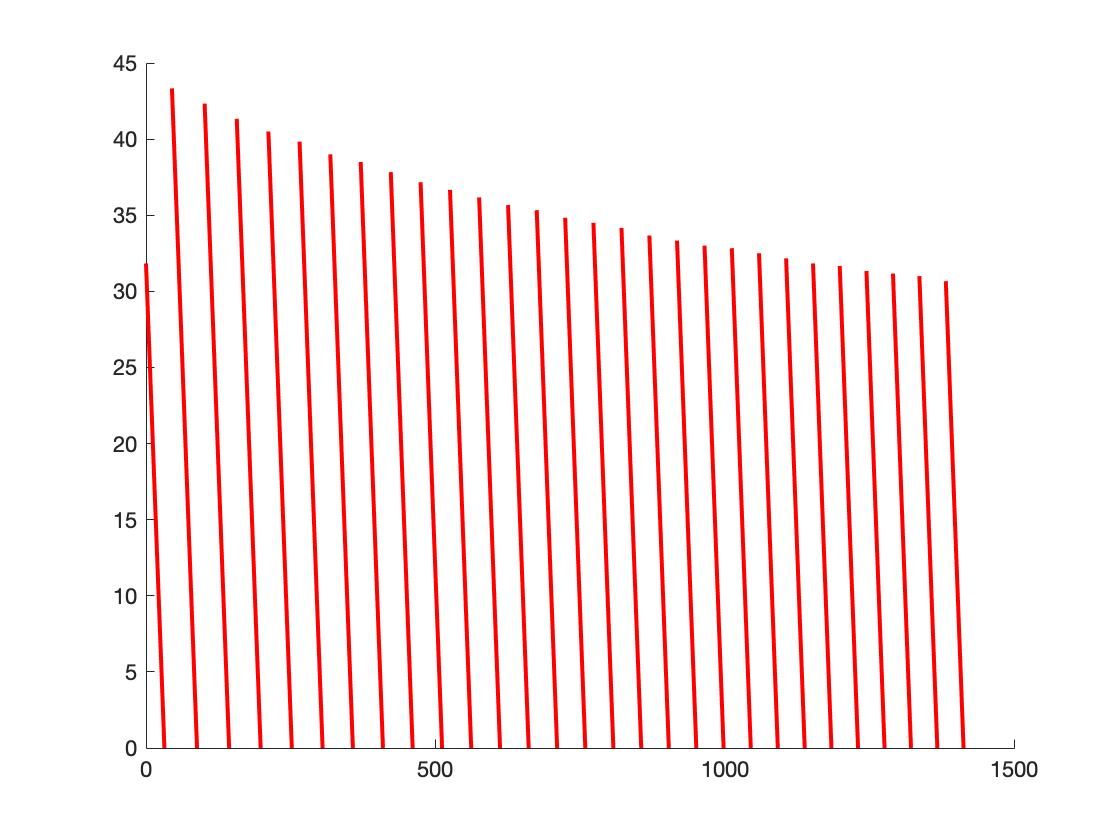
\includegraphics[width=1\textwidth]{figures/2-2-25-up.png}
    \subcaption{墙体13度,室外-25度,可上调时间曲线}
    \label{fig:my_label}
    \end{minipage}
\begin{minipage}[c]{0.35\textwidth}
    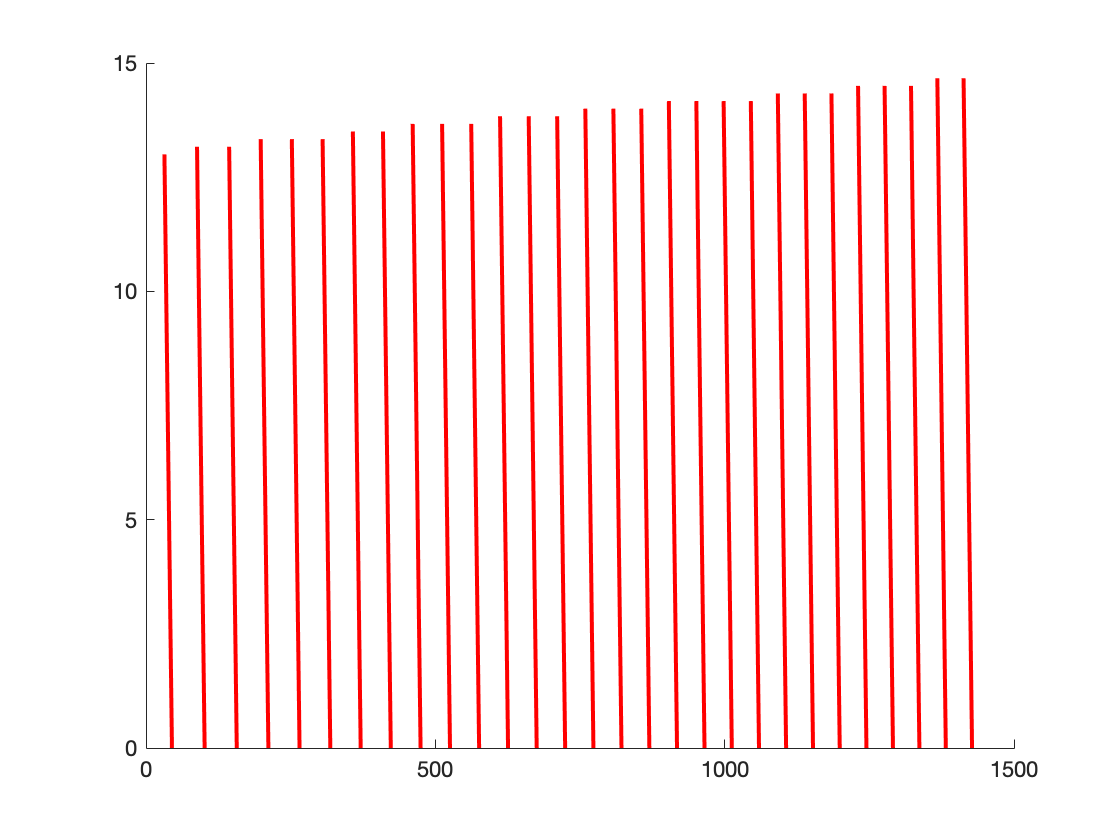
\includegraphics[width=1\textwidth]{figures/2-2-25-down.png}
    \subcaption{墙体13度,室外-25度,可	下调时间曲线}
    \label{fig:my_label}
\end{minipage}
 \caption{各个室外温度的可调节时间曲线}
\end{figure}

依据以上的计算结果,我们可以发现,虽然总体上可调节功率的时间曲线趋势是相似的,但随着室外温度下降,曲线会变得更加稀疏。并且可上调时间曲线的上界增大,可下调时间曲线上界减小。

也就是说,室外温度越低,功率可上调时间延长,可下调时间减短。整体上来看,可上调时间是越来越短的,可下调时间是越来越长的。

\subsection{问题三\quad 多个电采暖负荷的调节能力分析}
给定序号1-6的6个住户,室外温度-20度,室内初始温度在温控区间均匀分布,需要求出相应的电功率调节能力。本题假设开关初始状态均为开启(包括初始温度为22度的住户,第一次开启时间为0秒,也可以看作初始状态关闭)墙体初始温度均为15度。
\subsubsection{6个住户24h温度开关变化及总功率计算}
6个住户的室内初始温度分别为18.0,18.8,19.6,20.4,21.2,22.0度。分别计算每个住户的温度变化和开关状态,计算结果绘制如下图。
\begin{figure}[H]
    \centering
        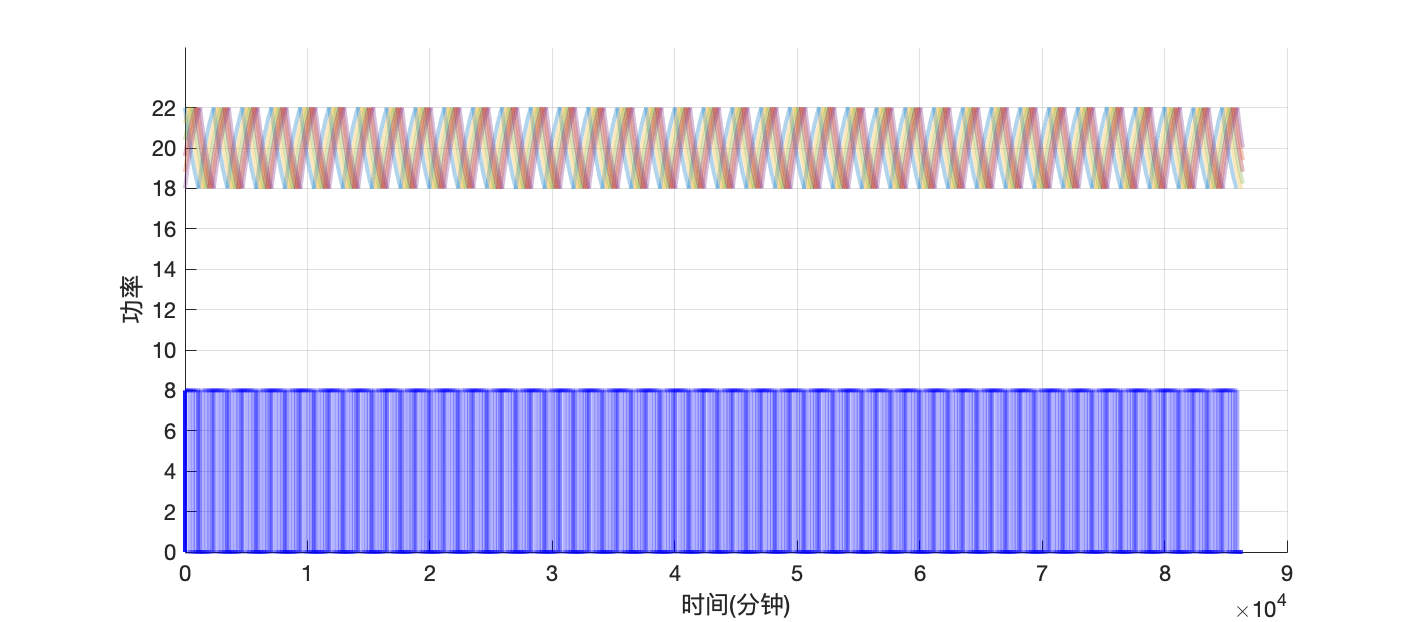
\includegraphics[width=1\textwidth]{figures/3-1.png}
    \caption{6名住户的温度变化及开关状态曲线}
    \label{fig:my_label}
    \end{figure}
    通过计算可以得到每个住户开启供暖的时间段,在计算结果上经过加和可以得到总功率曲线。
    \begin{figure}[H]
    \centering
        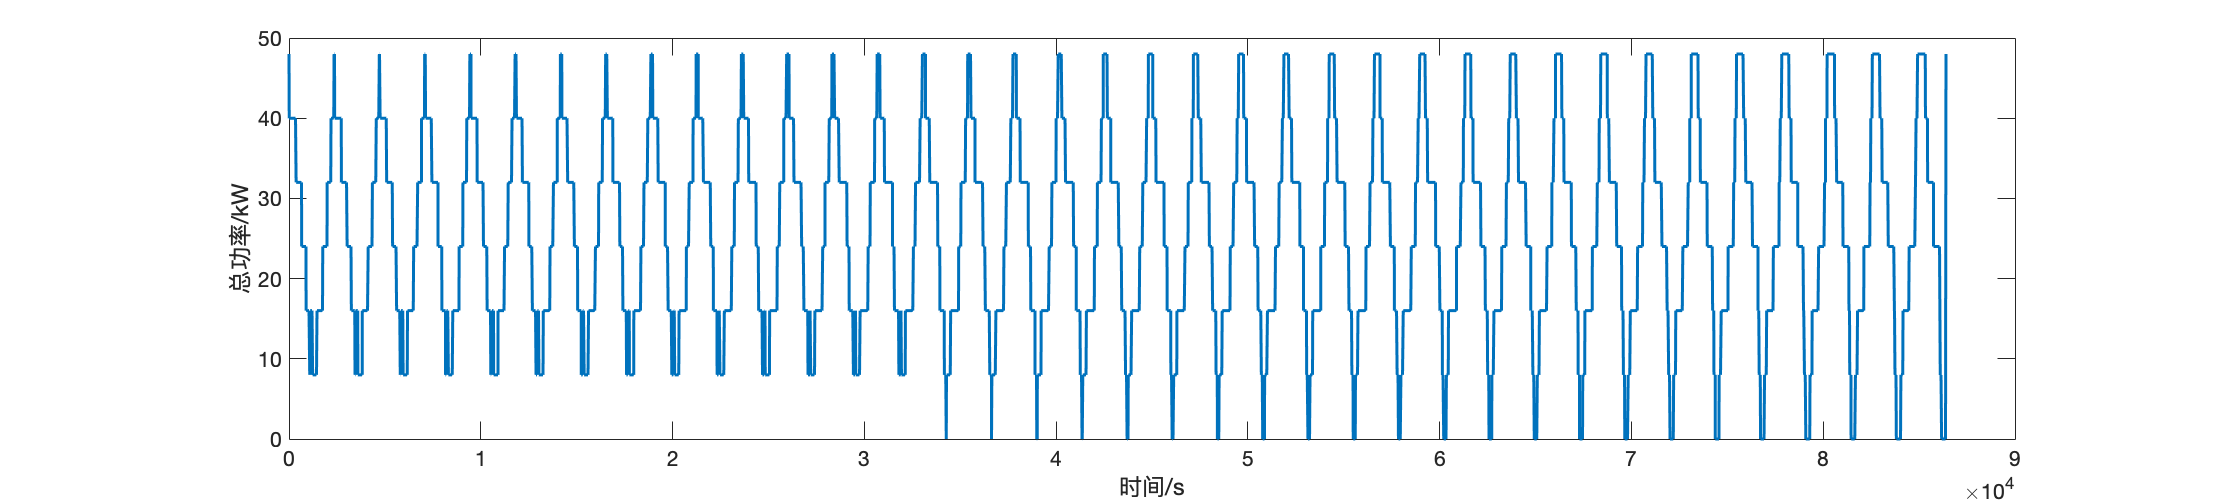
\includegraphics[width=1\textwidth]{figures/3-1-total.png}
    \caption{6名住户总功率曲线}
    \label{fig:my_label}
    \end{figure}
    \subsubsection{各时间点功率调节分析}
    以总功率曲线为基础,绘制了每分钟可参与调节功率的机器序号图,其中纵坐标轴代表序号,1-6分别对应了室内温度18-22度的住户,横坐标轴代表分钟为单位的时间点。
    \begin{figure}[H]
    \centering
        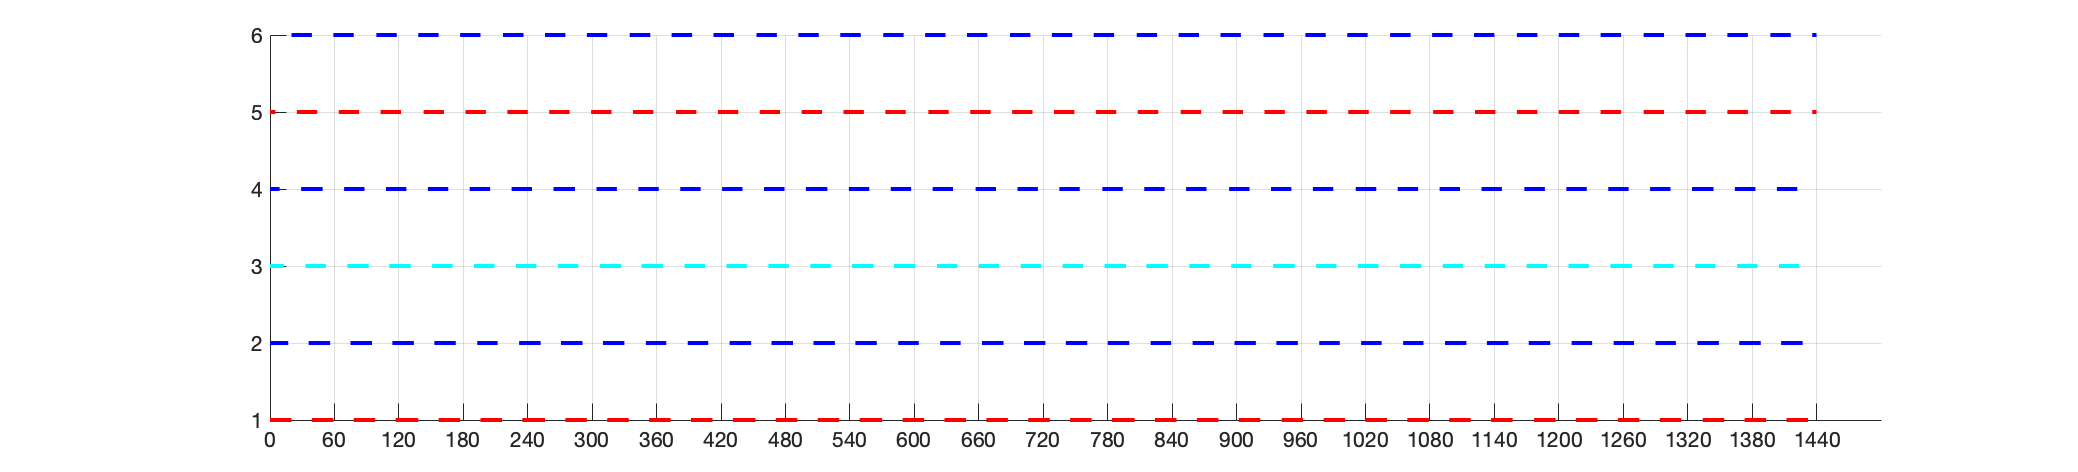
\includegraphics[width=1\textwidth]{figures/3-2-no.png}
    \caption{各时间点可参与上调电暖设备序号}
    \label{fig:my_label}
    \end{figure}
    
    \begin{figure}[H]
    \centering
        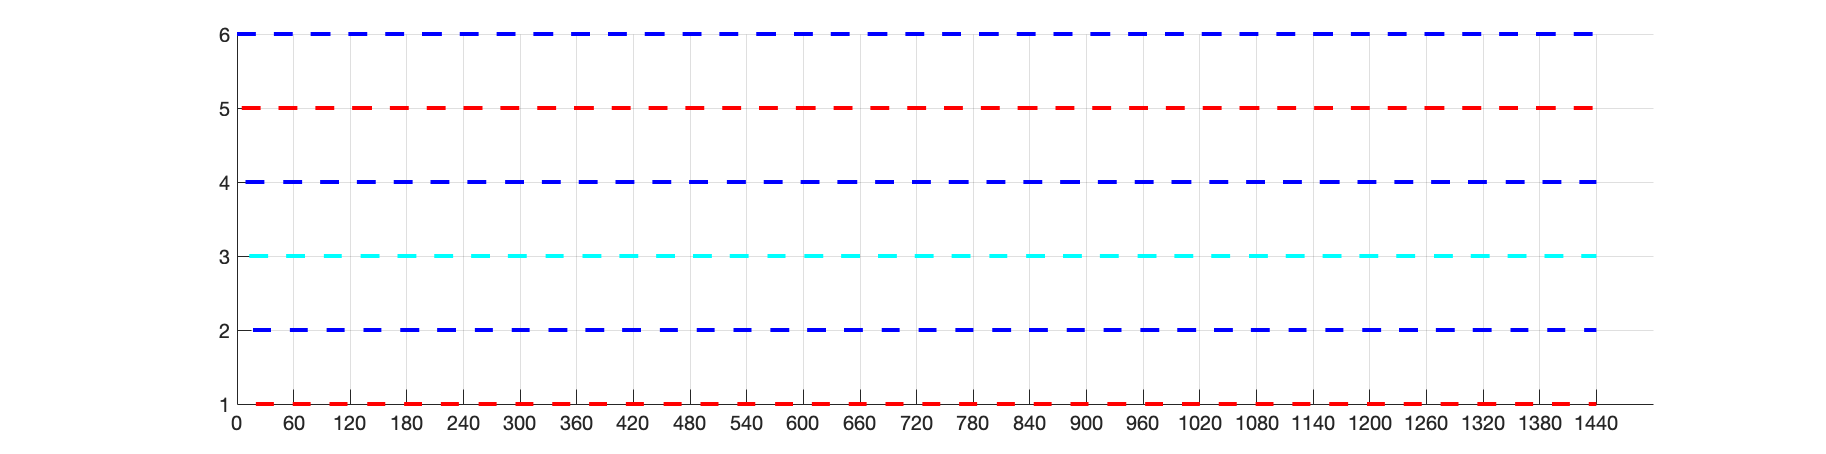
\includegraphics[width=1\textwidth]{figures/3-2-down.png}
    \caption{各时间点可参与下调电暖设备序号}
    \label{fig:my_label}
    \end{figure}
    
    绘制的各个时间点总可参与调节功率分别如下图所示。
      \begin{figure}[H]
    \centering
        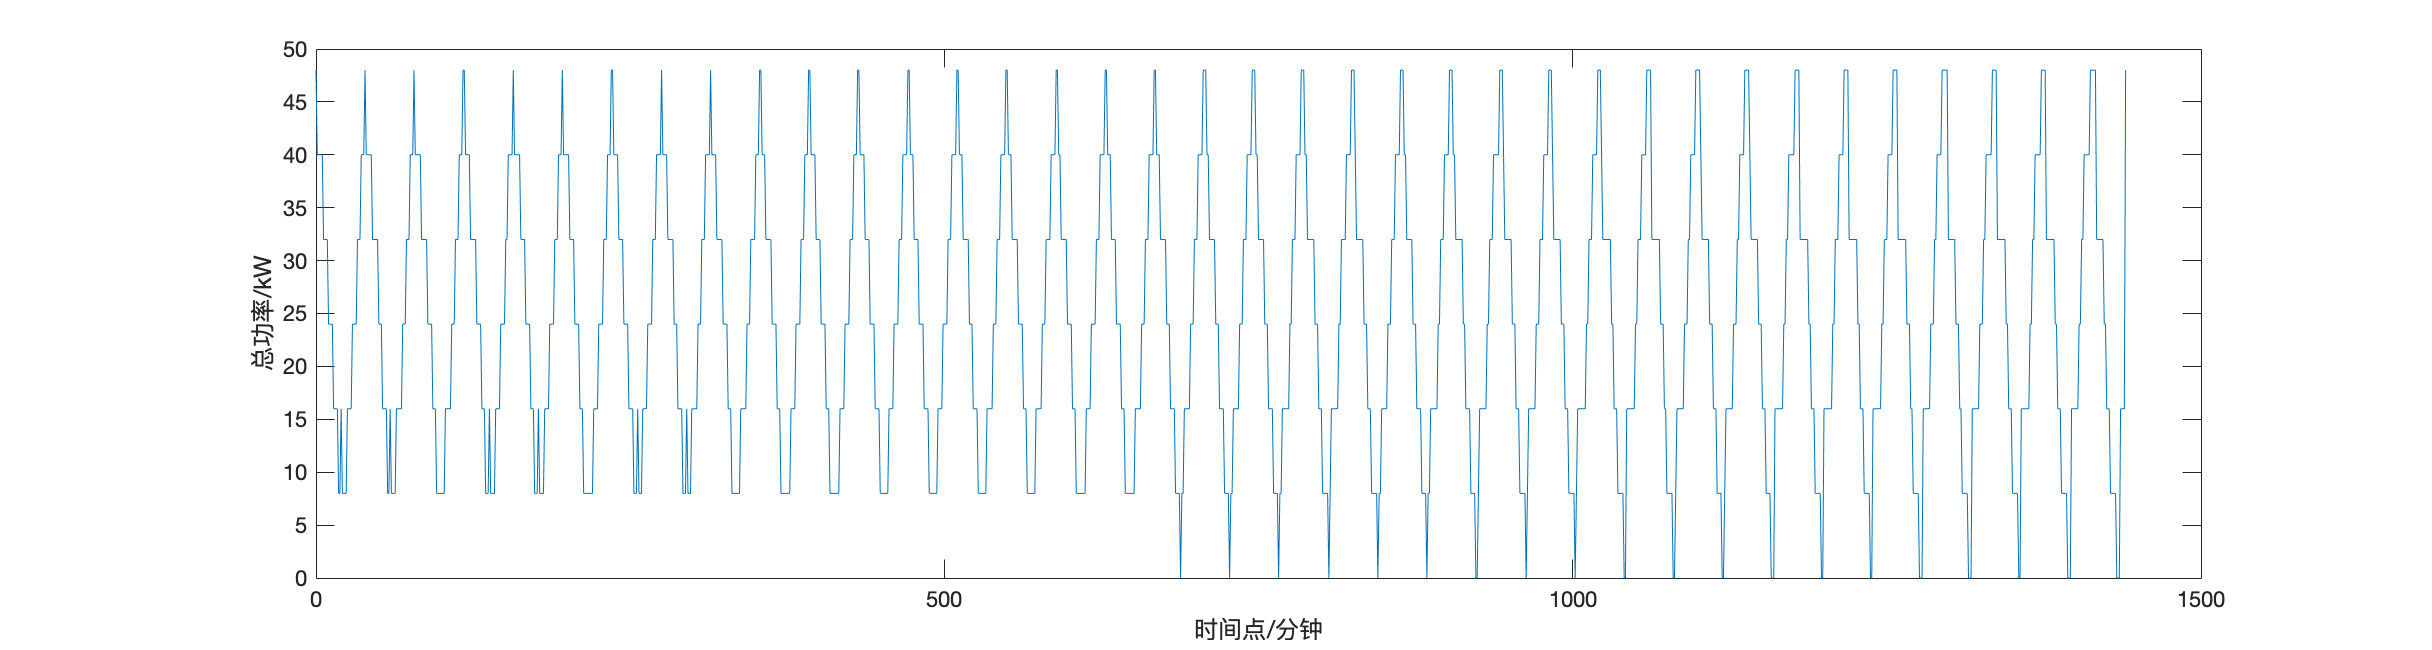
\includegraphics[width=1\textwidth]{figures/3-2-t-up.png}
    \caption{各时间点总可上调功率}
    \label{fig:my_label}
    \end{figure}
    
    \begin{figure}[H]
    \centering
        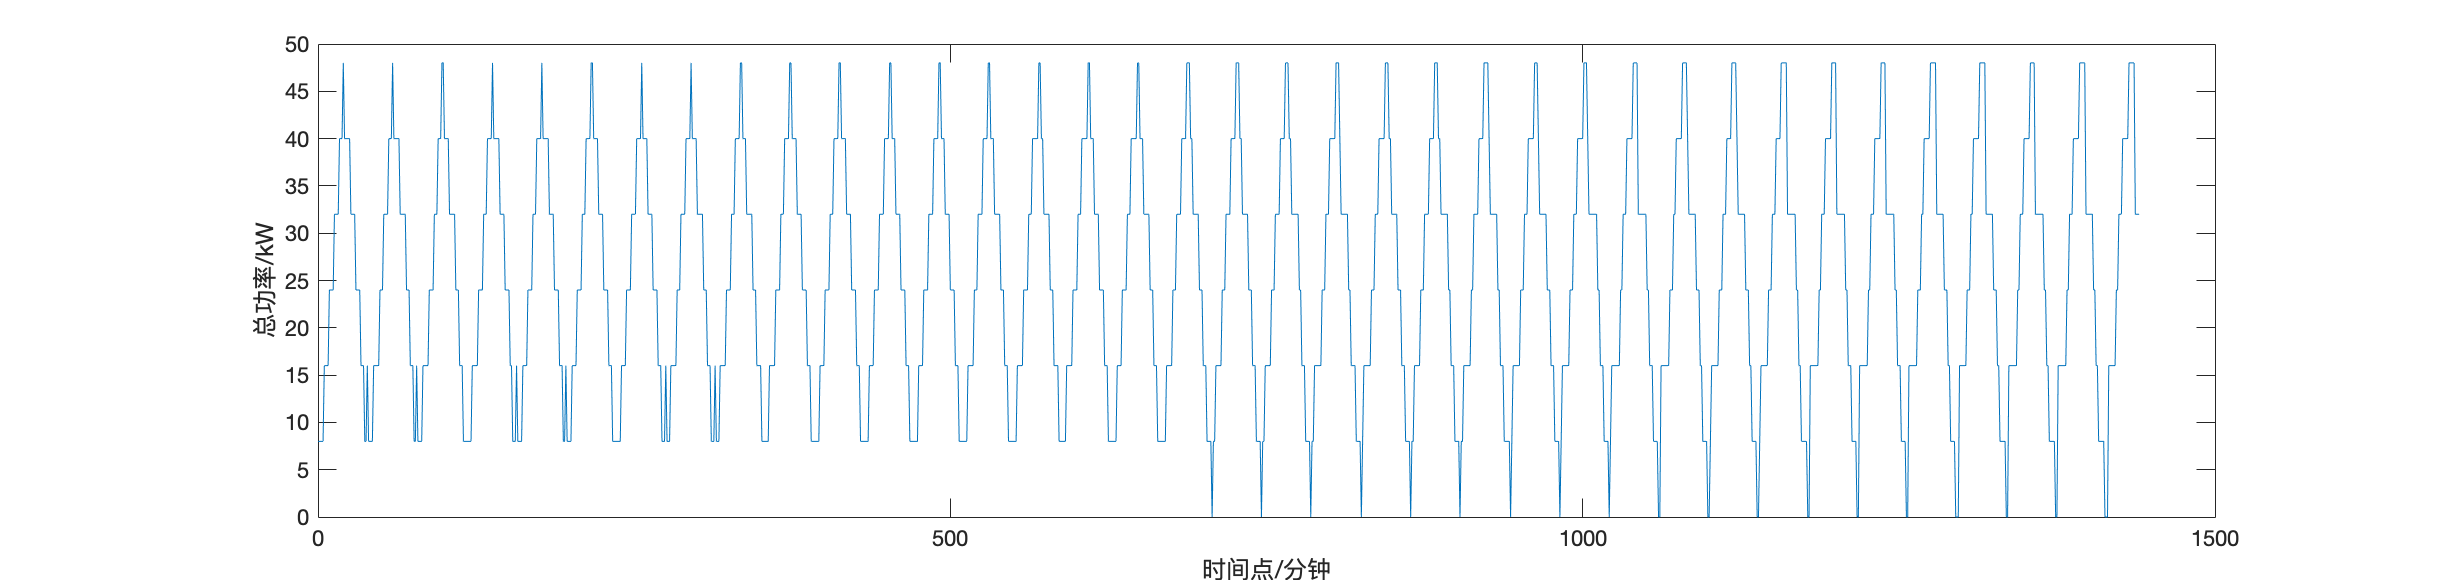
\includegraphics[width=1\textwidth]{figures/3-2-t-down.png}
    \caption{各时间点总可下调功率}
    \label{fig:my_label}
    \end{figure}
    
    \subsubsection{在不同室外温度下的分析}
    为了更好地展示室外温度的影响,保持其他条件不变,仅改变室外温度再次进行计算。选择室外温度为0,-5,-25度分别绘制了各时间点可调节功率的计算结果。
    
       \begin{figure}[H]
    \centering
        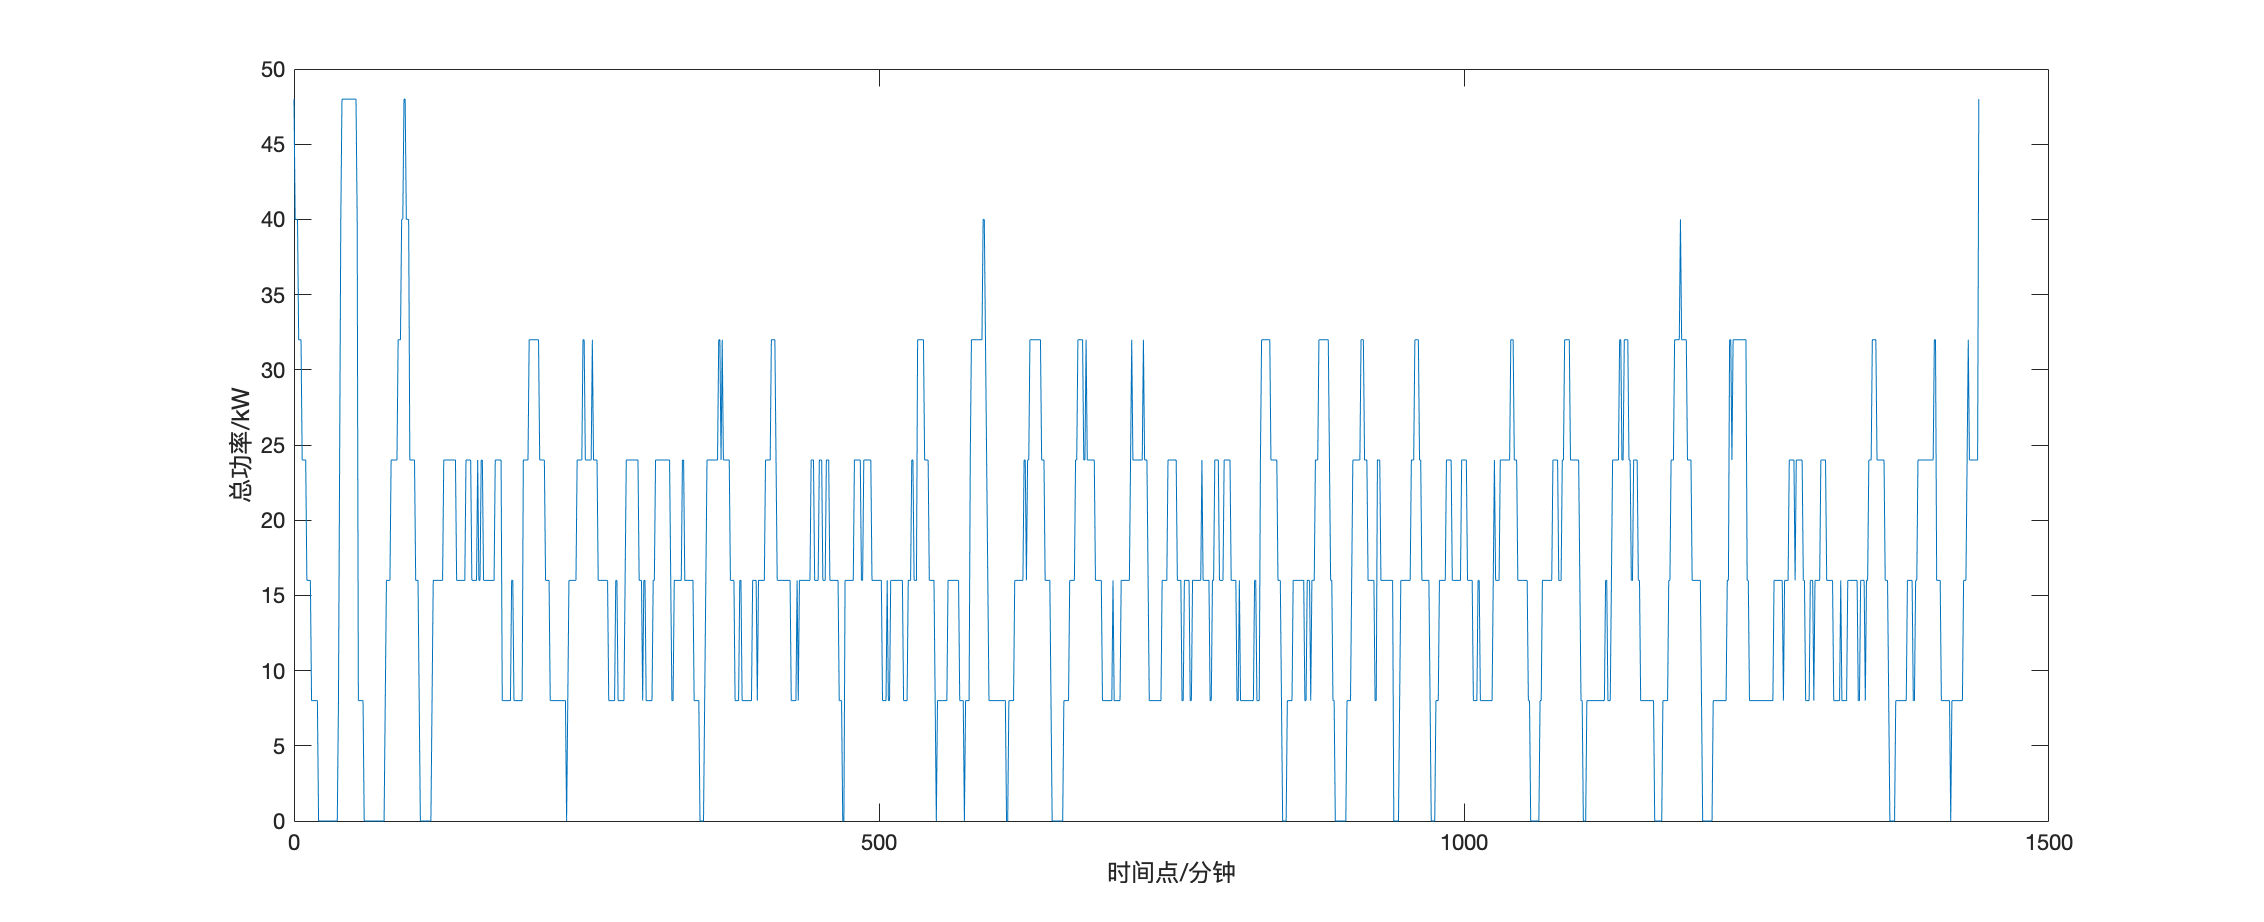
\includegraphics[width=1\textwidth]{figures/3-3-0.png}
    \caption{0度各时间点总可上调功率}
    \label{fig:my_label}
    \end{figure}
    
    \begin{figure}[H]
    \centering
        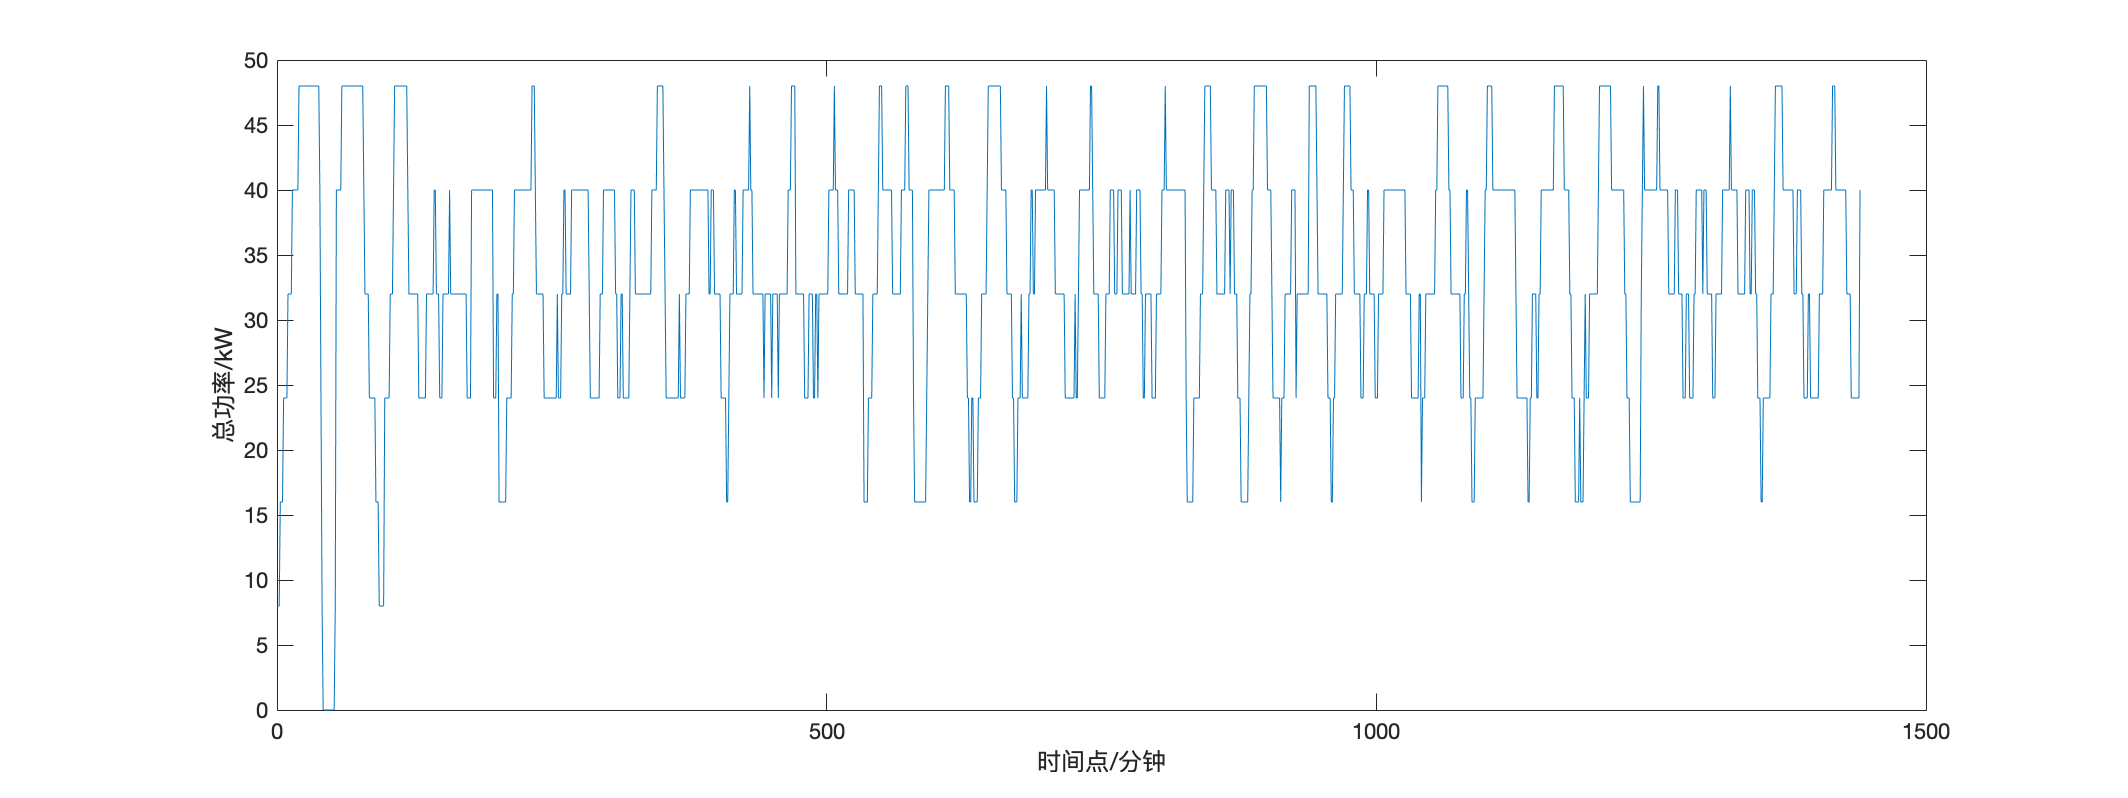
\includegraphics[width=1\textwidth]{figures/3-3-0-down.png}
    \caption{0度各时间点总可下调功率}
    \label{fig:my_label}
    \end{figure}
           \begin{figure}[H]
    \centering
        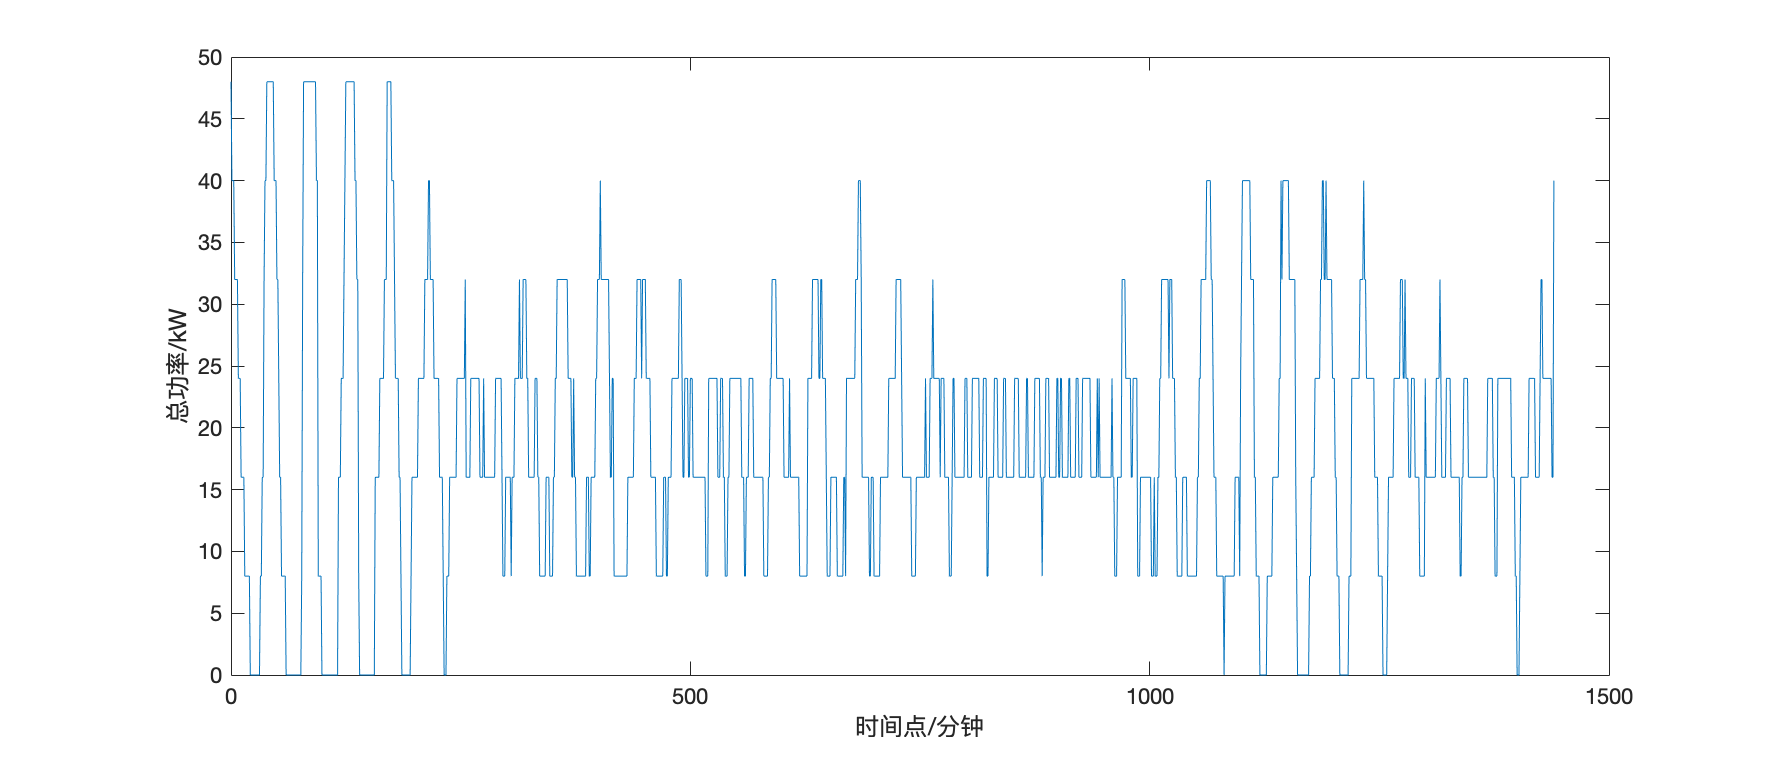
\includegraphics[width=1\textwidth]{figures/3-3-5-up.png}
    \caption{-5度各时间点总可上调功率}
    \label{fig:my_label}
    \end{figure}
    
    \begin{figure}[H]
    \centering
        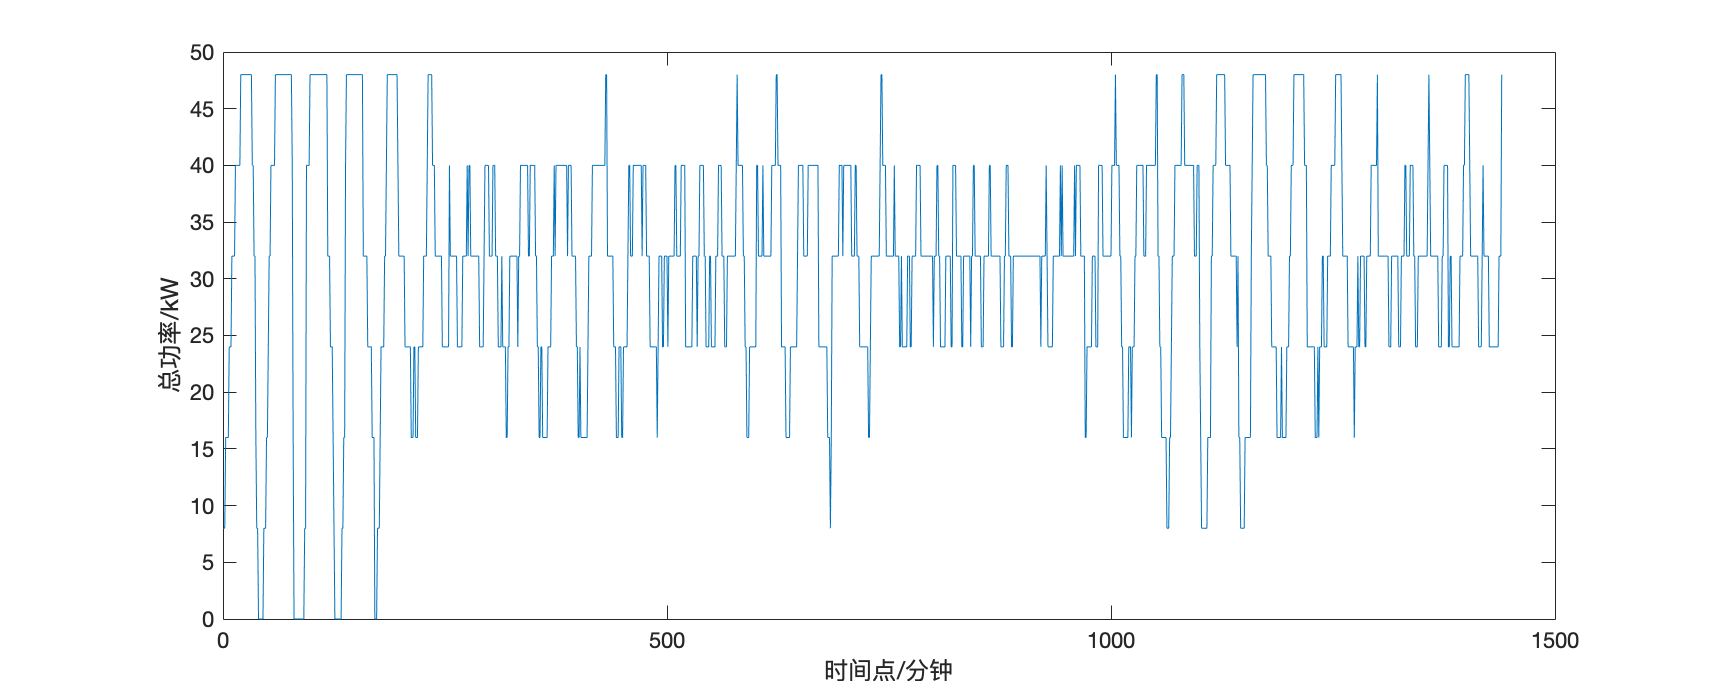
\includegraphics[width=1\textwidth]{figures/3-3-5-down.png}
    \caption{-5度各时间点总可下调功率}
    \label{fig:my_label}
    \end{figure}
               \begin{figure}[H]
    \centering
        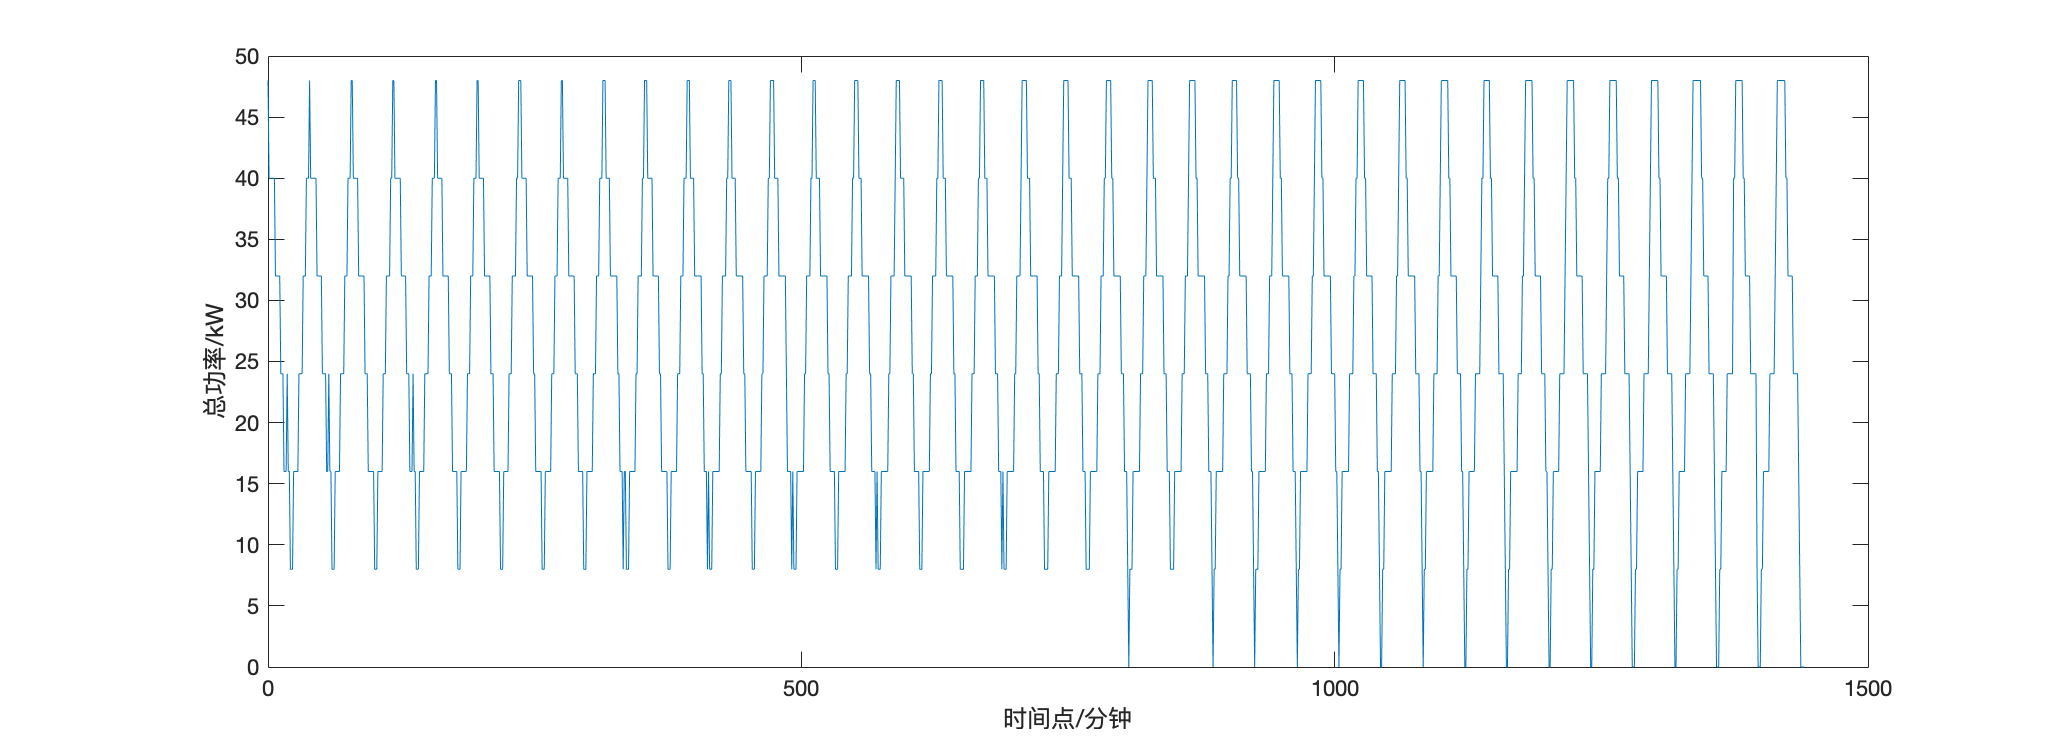
\includegraphics[width=1\textwidth]{figures/3-3-25-up.png}
    \caption{-25度各时间点总可上调功率}
    \label{fig:my_label}
    \end{figure}
    
    \begin{figure}[H]
    \centering
        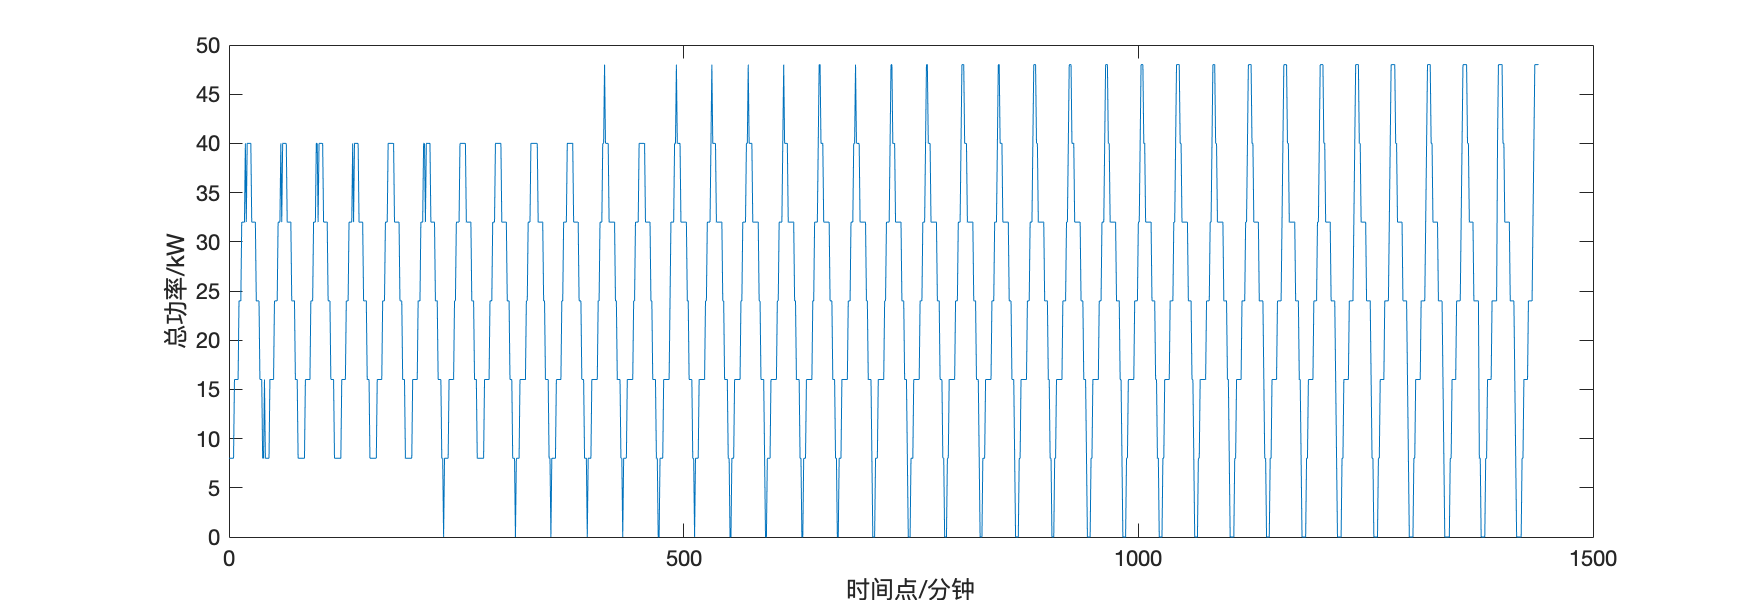
\includegraphics[width=1\textwidth]{figures/3-3-25down.png}
    \caption{-25度各时间点总可下调功率}
    \label{fig:my_label}
    \end{figure}
    根据图表展示的结果,我们发现室外温度对可调节功率的影响还是比较大的。
    
    当温度较高,如0度和-5度时,可上调功率总体较低,分布在图像下半部分,可下调功率总体较高,分布在图像上半部分。随着温度越来越低,在低温状态下,如-20度和-25度时,可调节功率的分布逐渐变得均匀,近似呈周期性波动状态。
    
    结合实际分析,在较高室外温度时,设备可上调功率较低,可下调功率较高,下调功率能力较强。在较低室外温度时,设备可参与调节的功率随着时间在最低点0和最高点48来回震荡,负荷高峰和低谷交错明显,参与上下调节的能力平均分布。
    
    \subsection{问题四\quad 住宅区电采暖负荷参与电网调节的能力分析}
    
   将上一问的分析结果推广到600住户的住宅区。室内初始温度服从温控区间内的均匀分布,开关初始状态均为开启,墙体初始温度为15度。
   
   以两个典型的室外温度为例子,室外温度-20度和0度时,分别计算24h内各时点可上调、下调的总功率如下所示:
\begin{figure}[H]
    \centering
        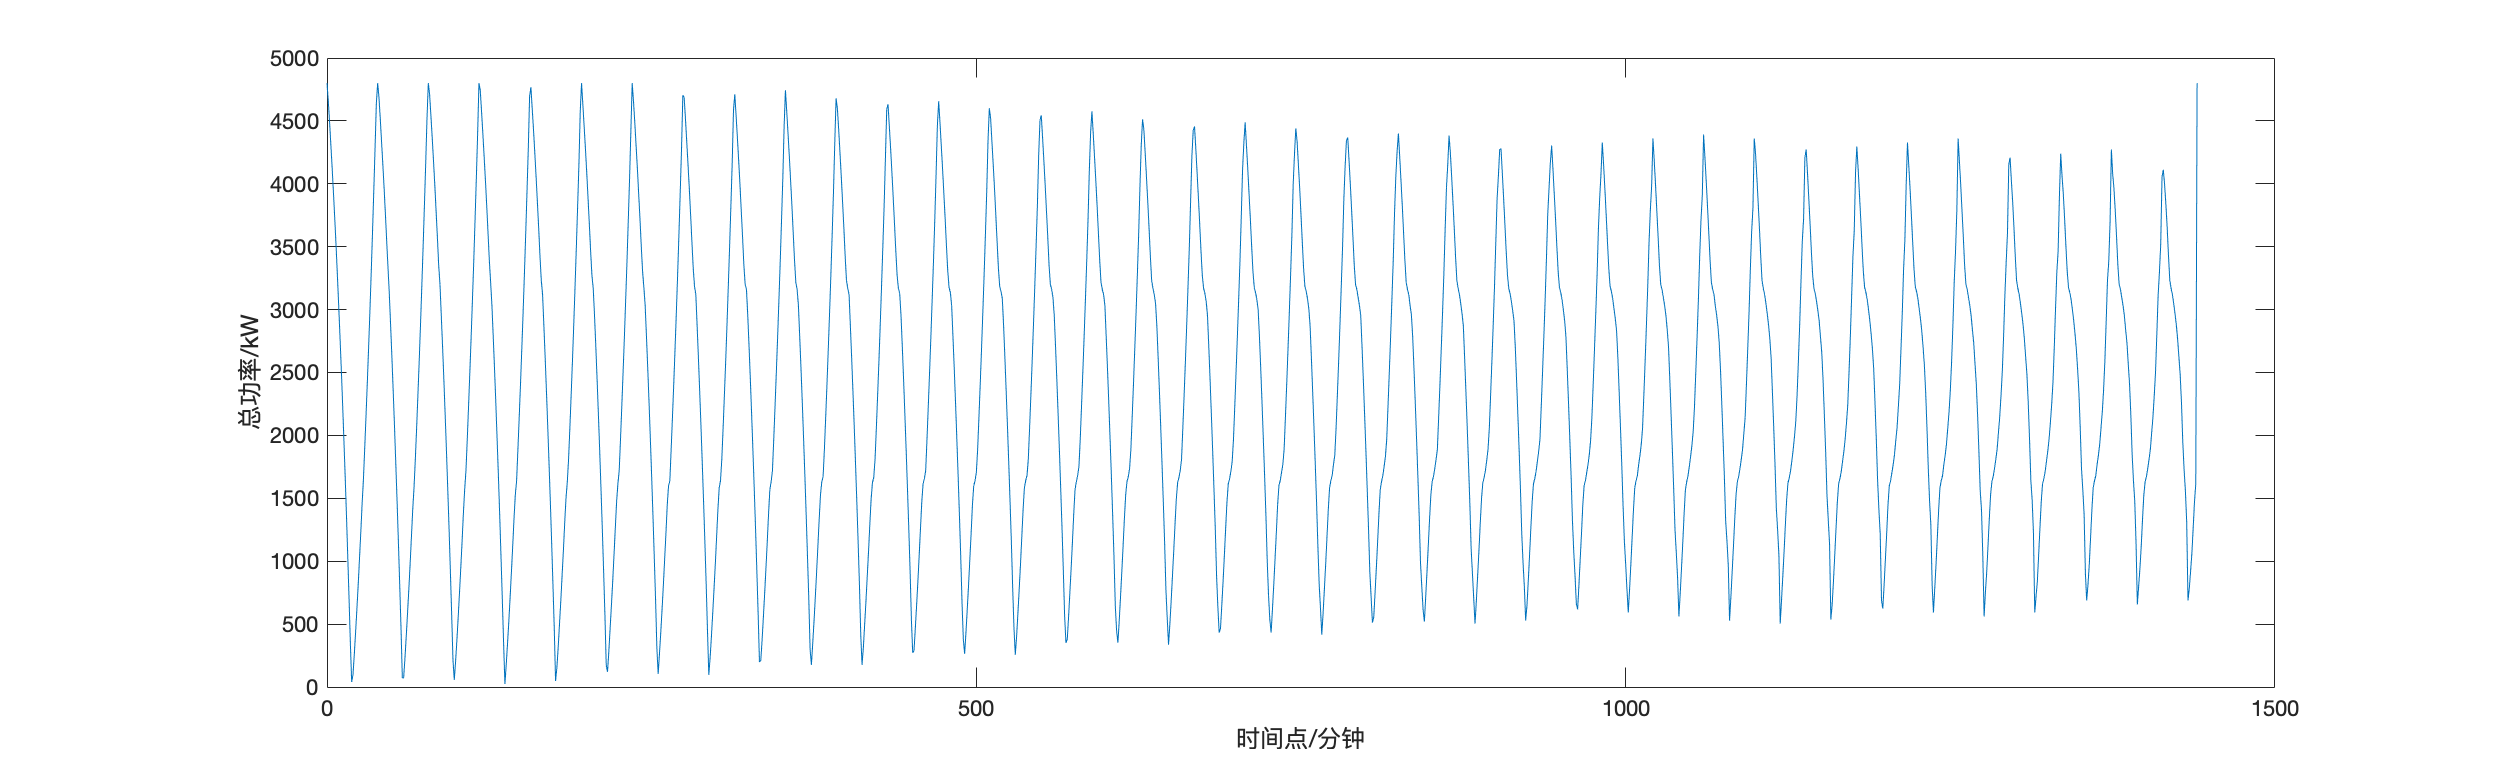
\includegraphics[width=1\textwidth]{figures/4-up.png}
    \caption{600户住户-20度各时间点总可上调功率}
    \label{fig:my_label}
    \end{figure}
    
    \begin{figure}[H]
    \centering
        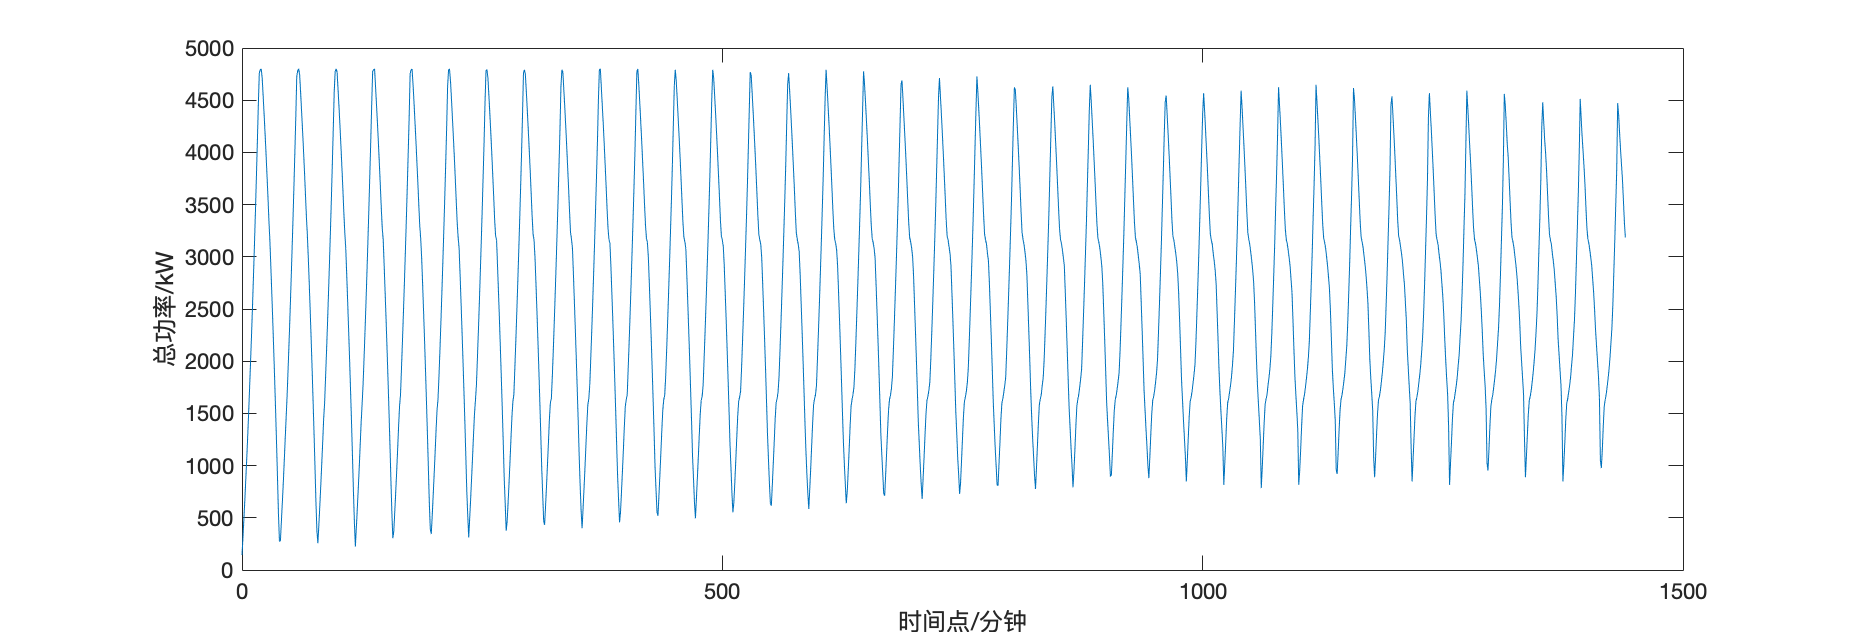
\includegraphics[width=1\textwidth]{figures/4-down.png}
    \caption{600户住户-20度各时间点总可下调功率}
    \label{fig:my_label}
    \end{figure}
    \begin{figure}[H]
    \centering
        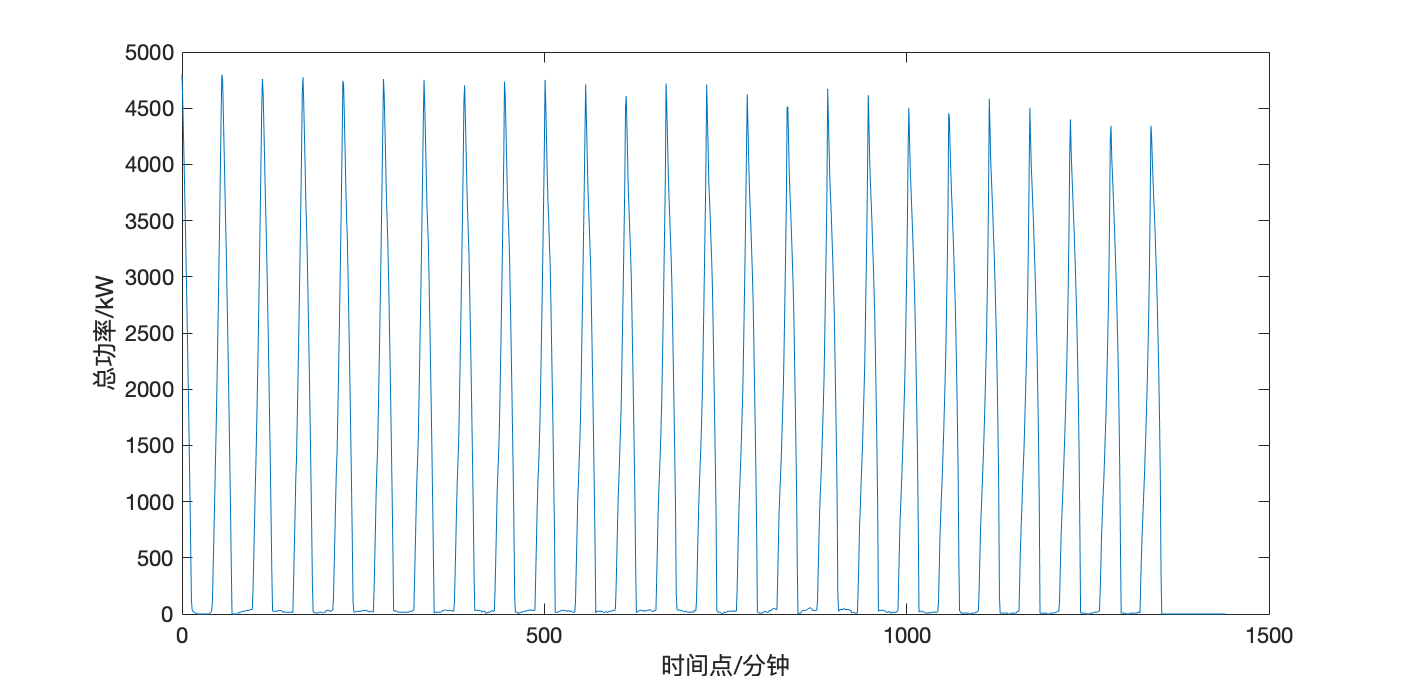
\includegraphics[width=1\textwidth]{figures/4-0-up.png}
    \caption{600户住户0度各时间点总可上调功率}
    \label{fig:my_label}
    \end{figure}
    
    \begin{figure}[H]
    \centering
        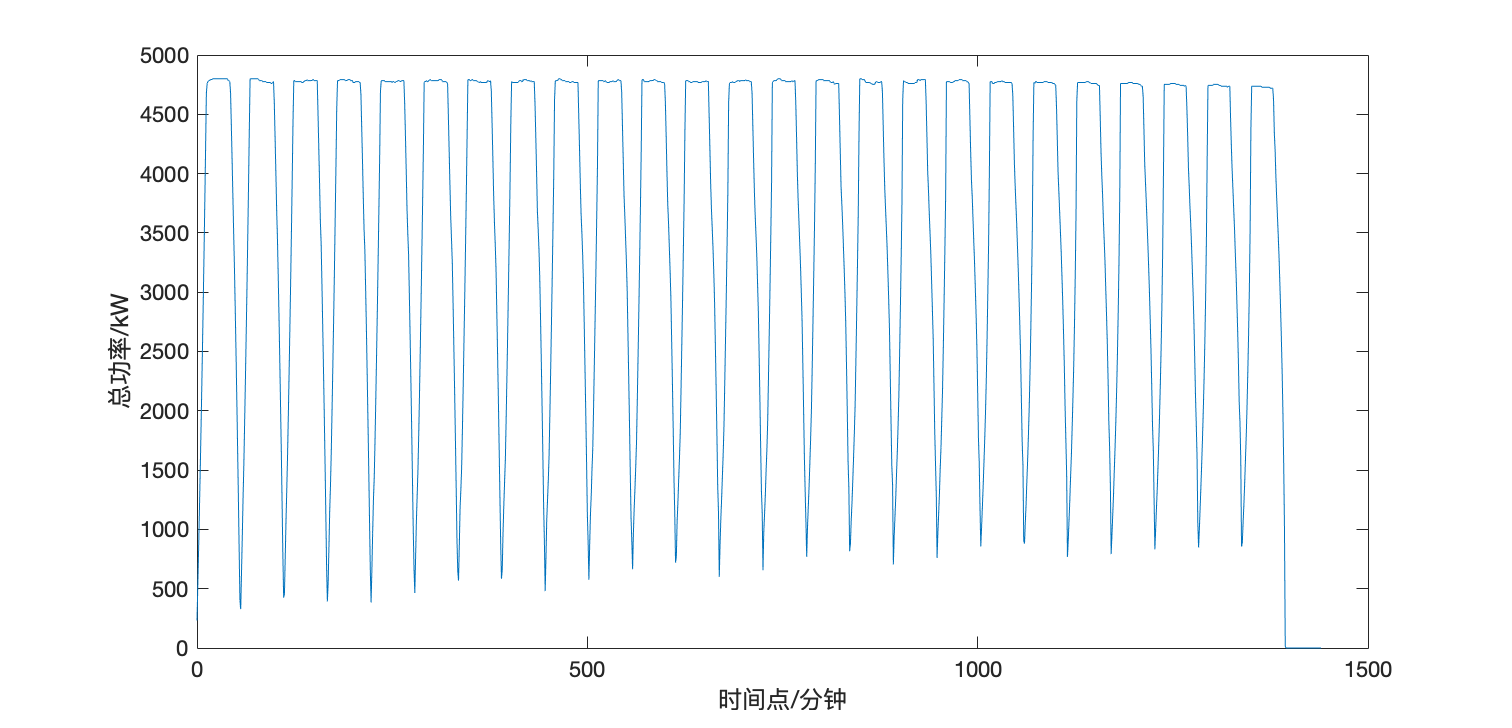
\includegraphics[width=1\textwidth]{figures/4-0-down.png}
    \caption{600户住户0度各时间点总可下调功率}
    \label{fig:my_label}
    \end{figure}
   总用功率如下图:
     \begin{figure}[H]
    \centering
        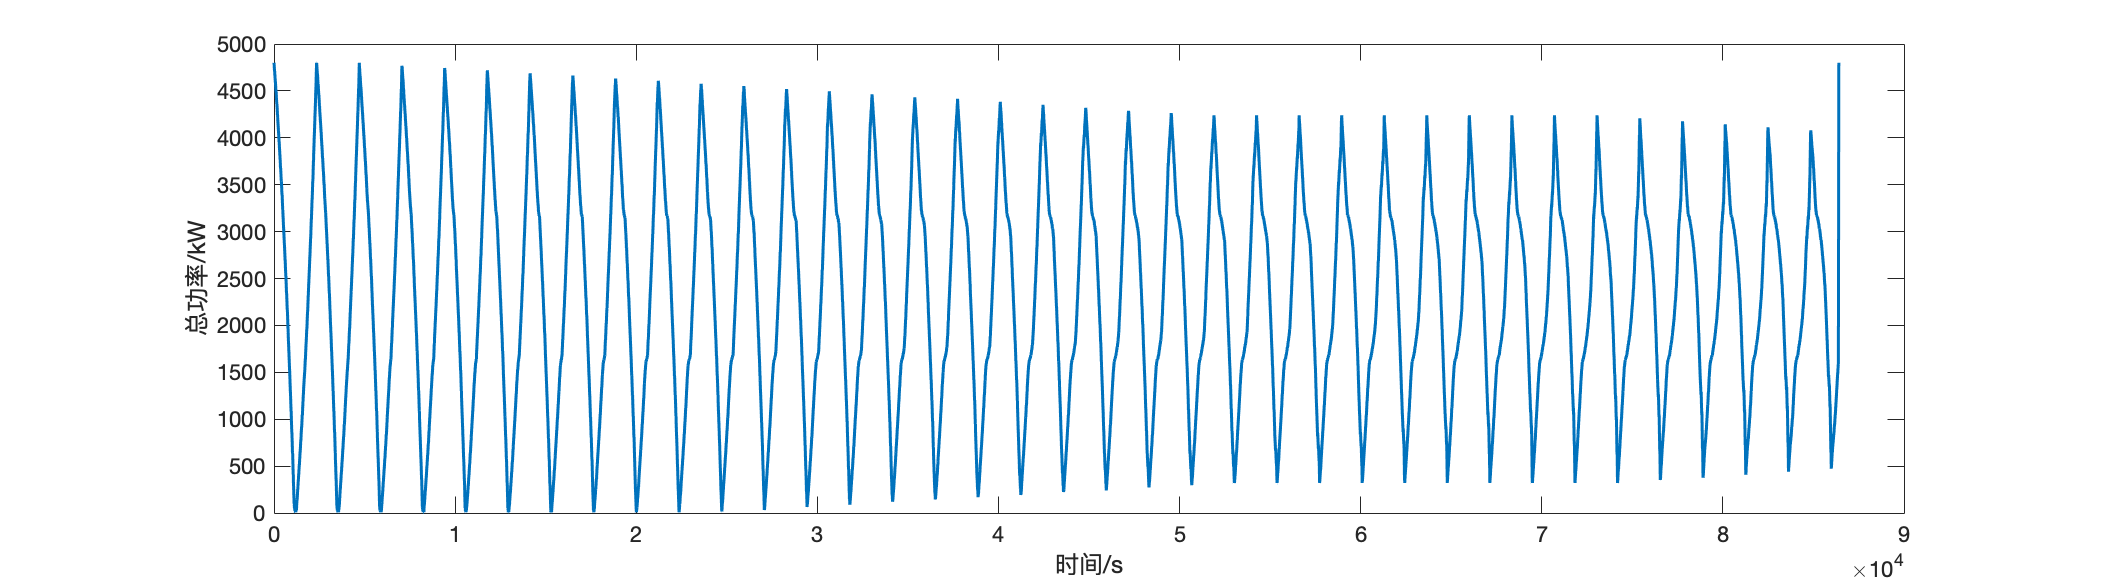
\includegraphics[width=1\textwidth]{figures/4-total.png}
    \caption{600户住户-20度各时间点总用功率}
    \label{fig:my_label}
    \end{figure}
    \subsection{问题五\quad 住宅区电采暖负荷参与电网削峰填谷的收益分析}
    由所给资料,削峰时间段为16到21时,填谷时间段为0到4时。以分钟为时间点,削峰时间段对应第960到1260个时间点,填谷时间段对应0到240时间点。
    \subsubsection{600户可提供持续最大向下调节功率值的计算}
    在削峰时间段,为了减小电量负荷,需要向下调节功率值。根据前面的计算,我们记$P_{total}(t)$为总功率函数,采用均值的方法计算$P_{Peak}$,在t为连续变量时有
    $$
    P_{Peak} =\frac{\int_{960}^{1260}P_{total}(t) \, dt}{1260-960} 
    $$
    由于题设t为分钟时间点,是离散变量,因此有等价的计算式:
    $$
    P_{Peak} =\frac{\sum_{t=960}^{1260} P_{total}(t)}{1260-960}  \\
    $$
        计算得到,各个室外温度对应的削峰时间段最大向下调节功率值如下:
    \begin{table}[H]
    \centering
    \begin{tabular}{|c|c|}\hline
 室外温度 &最大向下调节功率/kW \\ \hline
0	& 1137.7328 \\ \hline
-5 &	1242.7542  \\ \hline
-10&	 1418.0760\\ \hline
-15&  1744.4702\\ \hline
-20 &	2423.2242  \\ \hline
-25 &	2876.1391 \\ \hline
	\end{tabular}
\end{table}
以室外温度-20度为例,绘制削峰功率调节示意图。
\begin{figure}[H]
    \centering
        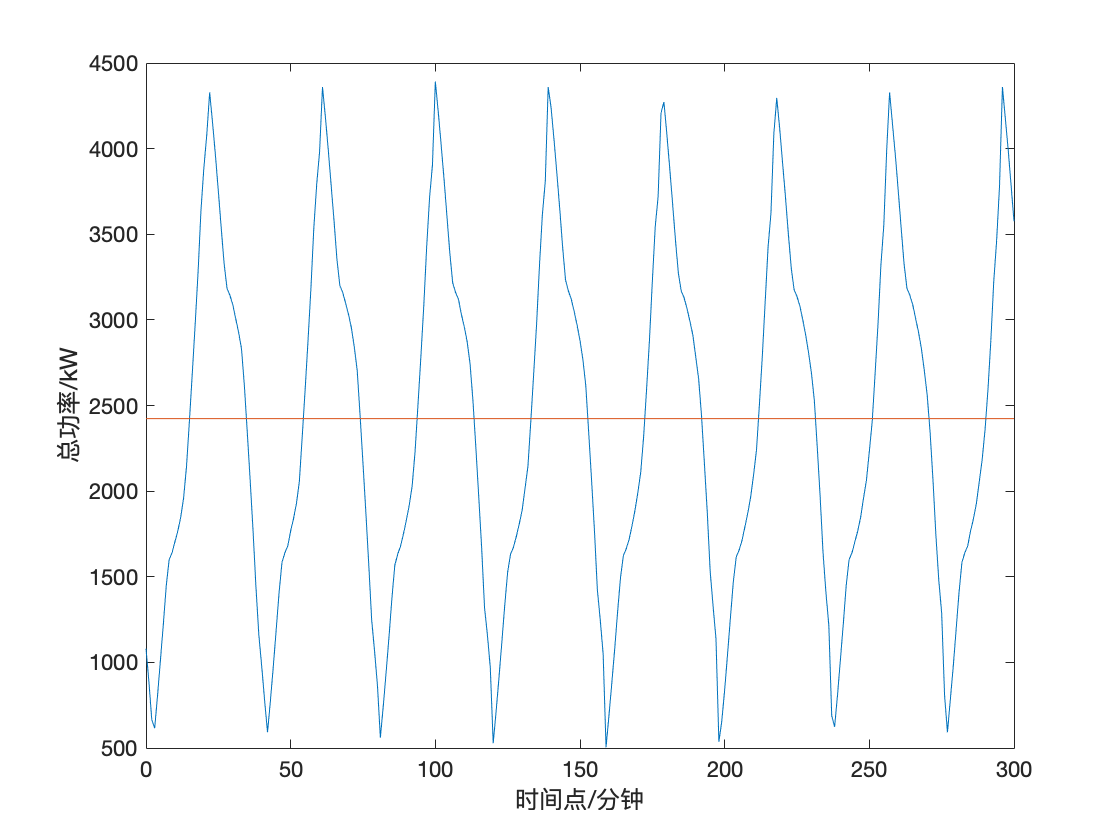
\includegraphics[width=1\textwidth]{figures/5-1-20.png}
    \caption{600户住户-20度削峰功率调节图}
    \label{fig:my_label}
    \end{figure}
    \subsubsection{600户可提供持续最大向上调节功率值的计算}
    填谷时持续调节功率计算方法为:
    $$
    P_{Valley} =\frac{\sum_{t=0}^{240} P_{total}(t)}{240-0}  \\
    $$
        \begin{table}[H]
            \centering
     \begin{tabular}{|c|c|}\hline
 室外温度 &最大向上调节功率/kW \\ \hline
0	&  3704.4 \\ \hline
-5 &	3699.6061    \\ \hline
-10&	3427.697 \\ \hline
-15&   3016.095  \\ \hline
-20 &	2477.1664  \\ \hline
-25 &	1708.224 \\ \hline
\end{tabular}
\end{table}

以室外温度-20度为例,绘制填谷功率调节示意图。
\begin{figure}[H]
    \centering
        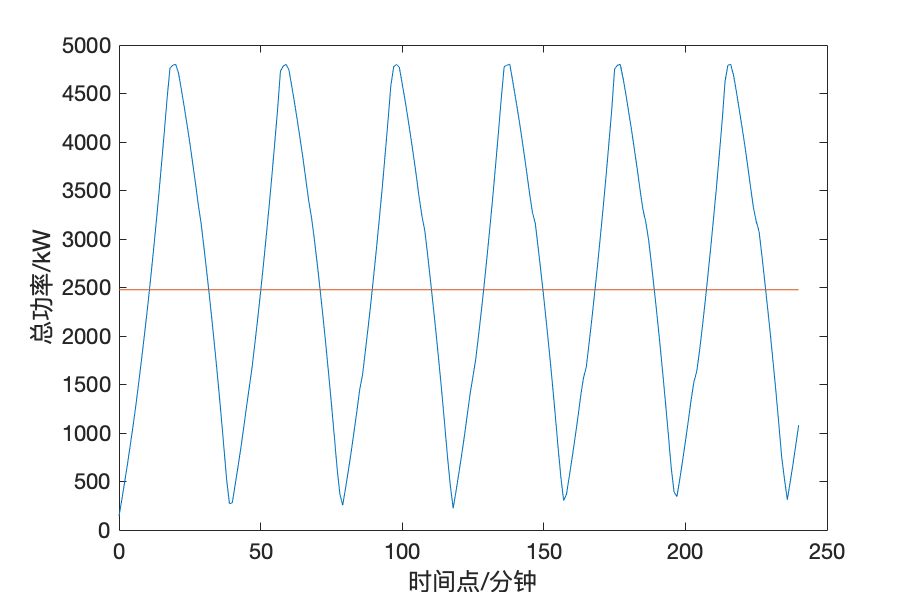
\includegraphics[width=1\textwidth]{figures/5-2-20.png}
    \caption{600户住户-20度填谷功率调节图}
    \label{fig:my_label}
    \end{figure}
    \subsubsection{开关状态受到功率调节影响的分析}
    因参与电网调节,需要改变住户的开关状态来控制功率在最大调节功率以内。计算每个时点因为参与调节而改变开关状态的方法如下,削峰时间段功率过高、需要向下调节时:
    $$
    \mbox{需要关闭的开关个数}n_{off} =\lceil \frac{ P(t)- P_{Peak} }{P_N}\rceil
    $$
    填谷时间段功率过低、需要向上调节时:
$$
    \mbox{需要打开的开关个数}n_{on} =\lceil \frac{ P_{Valley} -P(t)}{P_N}\rceil
    $$
    以-20度为例,绘制一段时间内参与电网调节的开关状态曲线。其中正值代表开启的开关数量,负值代表关闭的开关数量。
    \begin{figure}[H]
    \centering
        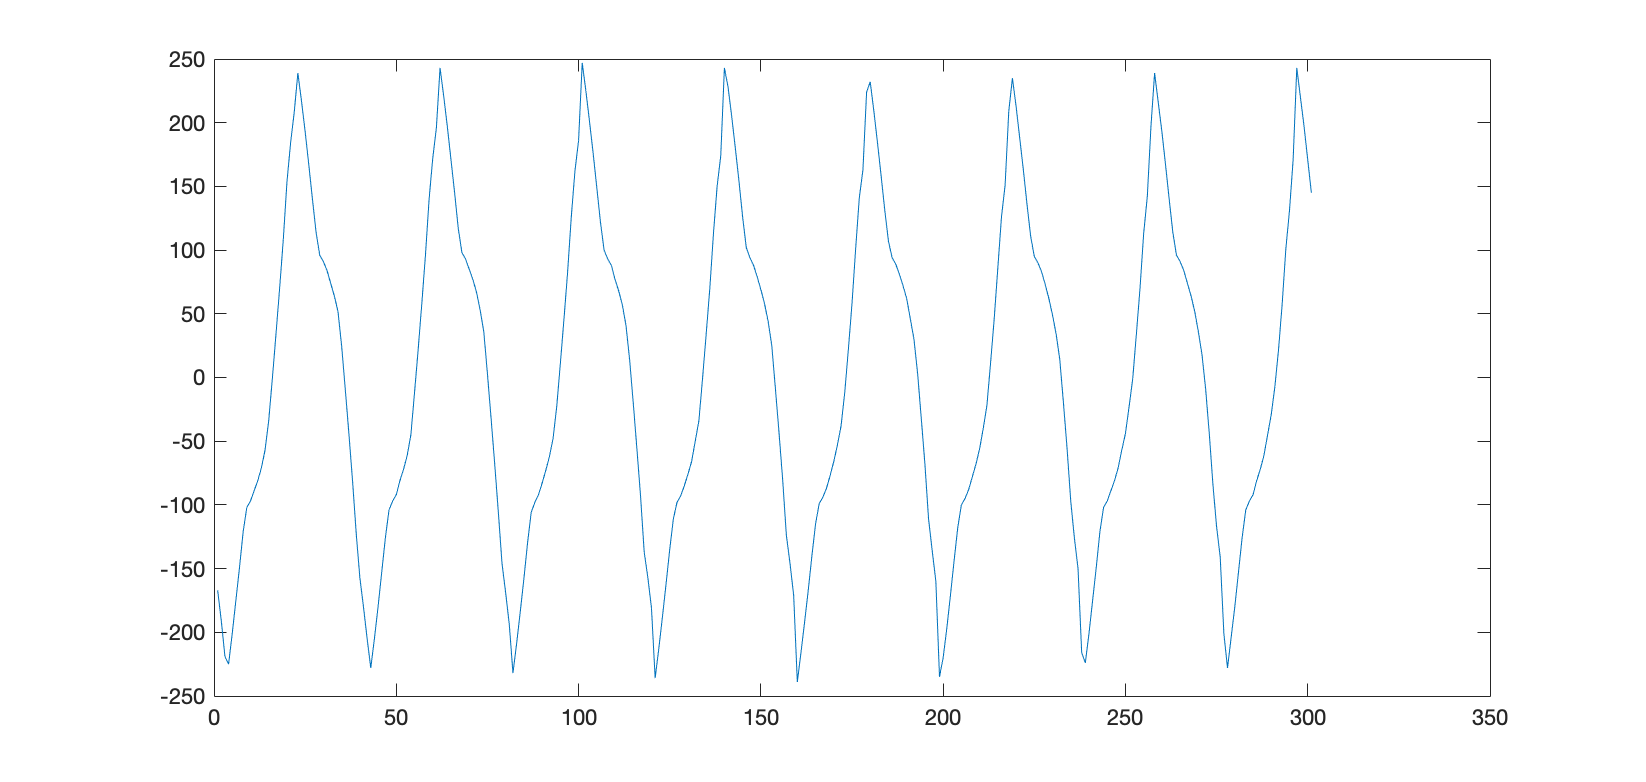
\includegraphics[width=0.8\textwidth]{figures/5-3-on.png}
    \caption{600户住户参与电网调节后的开关状态}
    \label{fig:my_label}
    \end{figure}
    绘制参与电网调节后的温度曲线,结果都在温控区间内。
    \begin{figure}[H]
    \centering
        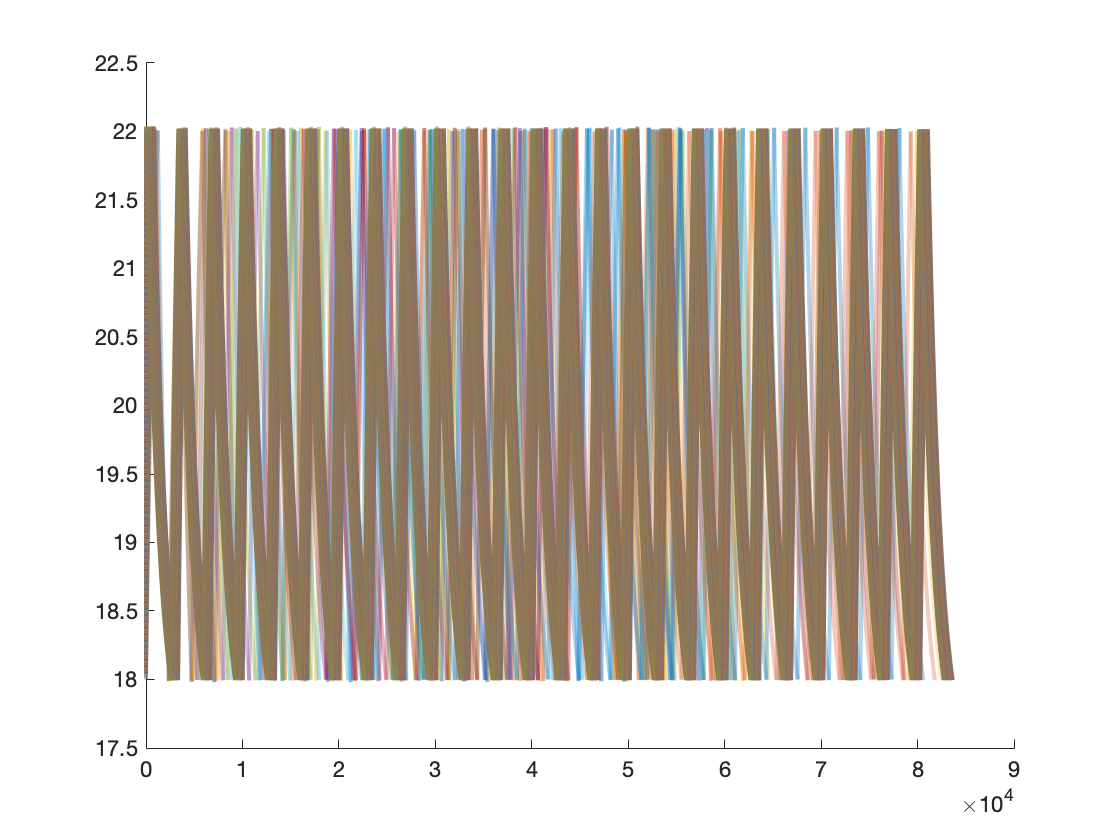
\includegraphics[width=0.8\textwidth]{figures/600-total-t.png}
    \caption{600户住户参与电网调节后的温度曲线}
    \label{fig:my_label}
    \end{figure}
\subsubsection{参与削峰填谷后供暖成本计算}
削峰补偿价格为1.30元/kWh,填谷补偿价格为0.65元/kWh,根据前两问估计的结果,可以计算出参与削峰填谷后的收益如下。
\begin{table}[H]
		\centering
\begin{tabular}{|c|c|c|c|c|}\hline
室外平均温度 &持续天数& 总收益 & 平均每户收益 &节省的成本/\% \\ \hline
0 $^\circ$C &30 &    566072.4 & 943.454 &  20.8445 \\ \hline
-5 $^\circ$C & 40& 863521.8 & 1439.203 & 21.48\\ \hline
  -10$^\circ$C &40 & 955974 & 1593.29& 18.33\\ \hline
   -15$^\circ$C &40 & 1076136 & 1793.56& 15.58\\ \hline
   -20$^\circ$C & 40&  1129434 &1882.39 & 17.907\\ \hline
    -25 $^\circ$C & 30 &869269.8 &1448.783& 22.233\\ \hline
    总计&180 & 5460408 & 9100.68 &18.9\\ \hline
\end{tabular}
\end{table}
因为本题计算量较大,结果为参考前面小问计算规律进行的估计,可能并不准确。但可以预计,在实现削峰填谷后,住户和工厂都会节省一定的成本,是非常好的策略。
\section{分析与展望}
\subsection{问题六\quad 温控型负荷参与电网调节展望}
\subsubsection{省级区域电采暖负荷参与电网调节的分析}
对于4000万平方米的省级供暖区域,面临的问题肯定会比小区住户要多,供暖方案的实现也比较麻烦。相对于小区域住户,可能遇到的问题有:
\begin{enumerate}
	\item 省级区域所涵盖的地域特征复杂,可能有平原和山区,不同的地理区域所需要的供暖强度不同,比如山区可能会比平原更加寒冷。
	\item 省级区域的经济水平参差不齐,需要考虑没有能力大规模、长期铺设供暖的情况。
	\item 省级区域人口密度不均匀,不同地区如何高效地利用土地,铺设供暖设备也是一大难点。
	\item 省级区域更容易产生大规模亏损,需要更加谨慎地设计节省成本的方案。
\end{enumerate}
针对省级区域供暖的困难,也提出了一些建议和解决方案。首先可以参考本文研究的削峰填谷方式进行供暖功率调节,节约成本。其次,分区域管理供暖设施,针对不同的区域设计不同的供暖方案。同时,若某区域出现供暖设备故障,不会影响到其他区域。
\subsubsection{南方空调的电功率分析}
不同于北方地区统一供暖,南方地区没有供暖系统,各家各户采用空调供暖,因此针对本文得到的结果并不能直接沿用。空调温控主要有以下的特点:
\begin{enumerate}
	\item 每家的开空调习惯、温度,空调品牌、安装方法等都有很大不同,不能实现供暖设备那种集体的调节。不同品牌、类型的空调,如挂壁式、中央空调、柜式空调,其用电方式都会有很大的不同。
	\item 制热方式不同,北方常见的暖气片主要通过自身升温缓慢提高周围温度,空调则是通过吹风实现改变温度。
	\item 能耗与使用习惯不同,北方的供暖由于能耗低、升温缓慢,会一直开着暖气片,使室内温度一直维持在一个比较舒适的区间。而南方的空调因为能耗更高、升温较快,大部分家庭会选择在需要的时候才开启,而不会一直开启。
	\item 南方天气较北方比较潮湿多雨,也会影响到空调的用电情况。
\end{enumerate}

\subsection{模型评价}
本文的核心围绕着解决房间温变过程的微分方程展开。该方程理论上可以通过软件求得精确解,但比较繁琐,且在现实生活中不需要精确到秒以内,因此本文选择解决数值解来替代解方程,这样的结果是程序运行效率较高,但同时不会非常精确。不过该方法并不是完全最优,在计算600户的结果时仍然十分缓慢,因此如何更高效地解决方程,是一个值得继续讨论的点。

此外,可能因为存在理想化假设,计算结果或许有着较大的偏差。若需要实际应用,还要考虑多方面的问题。
%参考文献
\newpage
\begin{thebibliography}{9}%宽度9
\bibitem{d}丁国栋. 计及电热时序耦合特性的电热联合系统源荷协同调度[D].东北电力大学,2022.
\bibitem{l}李明,郑云平,印欣等.考虑用户舒适度的分散式电采暖调峰优化控制[J/OL].南方电网技术,2023.
\bibitem{w}王甜甜. 基于多目标优化的分布式电采暖控制策略研究[D].东北电力大学,2022.
\bibitem{c}陈灵,黄兴华,张功林等.考虑削峰填谷的分布式电源集群协同控制方法[J].智慧电力,2023.
\end{thebibliography}

\newpage
%附录
\begin{appendices}

\section{源码}

求解微分方程解析解代码:
\begin{lstlisting}[language=matlab]
syms t n c1 c2 r1 r2 x0 y0 Pn Tout
[x3,y3] = dsolve('Dx = Pn+(-1/(c1*r1))*(x-y)', 'Dy =(1/(c2*r1))*(x-y)-(1/(c2*r2)*(y-Tout))','x(0)=x0','y(0)=y0');
\end{lstlisting}

方程函数文件
\begin{lstlisting}[language=matlab]
function  xprim=f2(t,x)
xprim=[(-1/(1.1e6*1.2e-3))*(x(1)-x(2));
(1/(1.86e8*1.2e-3))*(x(1)-x(2))-(1/(9.2e-3*1.86e8)*(x(2)))];
function  xprim=f(t,x)
xprim=[(8e3/1.1e6)+(-1/(1.1e6*1.2e-3))*(x(1)-x(2));
(1/(1.86e8*1.2e-3))*(x(1)-x(2))-(1/(9.2e-3*1.86e8)*(x(2)+0))];
\end{lstlisting}
绘制各个时间点可参与调节的住户序号
\begin{lstlisting}[language=matlab]
hold on
for i = 1:2:75
    
    plot([time_floor(1,i),time_floor(1,i+1)],[1,1],'r','LineWidth',2)
    plot([time_floor(2,i),time_floor(2,i+1)],[2,2],'b','LineWidth',2)
    plot([time_floor(3,i),time_floor(3,i+1)],[3,3],'c','LineWidth',2)
    plot([time_floor(4,i),time_floor(4,i+1)],[4,4],'b','LineWidth',2)
    plot([time_floor(5,i),time_floor(5,i+1)],[5,5],'r','LineWidth',2)
    plot([time_floor(6,i),time_floor(6,i+1)],[6,6],'b','LineWidth',2)
end
xticks(0:60:1440)
hold off
grid on
\end{lstlisting}
绘制各个时间点总可调节功率曲线
\begin{lstlisting}[language=matlab]
total_up_minute = [];
sum_up_power = linspace(0,0,1441);
for i =1 :1:6
    minute_up = linspace(0,0,1441);
    for j = 2 :2 :75
    n = time_floor(i,j);
    n2 = time_floor(i,j+1);
    minute_up(n+1:1:n2+1) = 1;
    end
    total_up_minute= [total_up_minute;minute_up];
    sum_up_power = total_up_minute(i,:) + sum_up_power;
end
plot(linspace(0,1440,1441),8* sum_up_power)
xlabel('时间点/分钟')
ylabel('总功率/kW')
\end{lstlisting}
计算温度曲线的主程序:
\begin{lstlisting}[language=matlab]
%先开后关
t0 = 0;
res = [];
time = [];
q = 15;
time_index = [0];%存放t0的索引
wall_res = [];
total_res = [];
q0= 18.8;
for n = 1:1:37
    [tn,xn] = ode45('f',[t0:10: 24*60*60],[q0;q]);
    length1 = size(xn);
    for in = 1:1:length1(1)
    if xn(in) >= 22 
    break
    end
    end
    t0 = tn(in);
    q = xn(in,2);
    res = [res;xn(1:1:in,1)];
    wall_res = [wall_res ; xn(1:1:in,2)];
    time = [time;tn(1:1:in,1)];
    time_index = [time_index t0];
    [tn2,xn2] = ode45('f2',[t0:10: 24*60*60],[22;q]);
    length = size(xn2);
    for in2 = 1:1:length(1)
    if xn2(in2) <= 18
        break
    end
    end
    t0 = tn2(in2);
    q = xn2(in2,2);
    res = [res;xn2(1:1:in2,1)];
    wall_res = [wall_res ; xn2(1:1:in2,2)];
    time = [time;tn2(1:1:in2,1)];
    time_index = [time_index t0];
    q0 = 18;
   
end

%subplot(2,1,1)
hold on
plot1=plot(time,res,'LineWidth',2);
plot1.Color(4) =0.3;

%plot(time,wall_res,'LineWidth',2);
%plot( t([1:1:i]),x([1:1:i]));
%subplot(2,1,2)
t_on = 0;
t_off = 0;
time_index_s =time_index;


for i = 1: 2 : 74

plot_a = plot([time_index(i),time_index(i+1)],[8,8],'b','LineWidth',2);
plot_a.Color(4) = 0.3;
t_off = t_off + (time_index(i+1)-time_index(i));
plot_b = plot([time_index(i),time_index(i)],[8,0],'b','LineWidth',2);
plot_b.Color(4) = 0.3;
plot_c = plot([time_index(i+1),time_index(i+1)],[8,0],'b','LineWidth',2);
plot_c.Color(4) = 0.3;
plot_d = plot([time_index(i+1),time_index(i+2)],[0,0],'b','LineWidth',2);
plot_d.Color(4) = 0.3;
t_on = t_on + (time_index(i+2)-time_index(i+1));
end
%xticks(time_index)
%legend('室内温度','墙体温度','功率');
yticks(0:2:22);
xlabel('时间(分钟)');
ylabel('功率');

grid on;

hold off

for i = 1: 2 : 58
plot([time_index(i),time_index(i+1)],[time_index(i+1)-time_index(i),0],'r','LineWidth',2);
end

for i = 1: 2 : 58
plot([time_index(i+1),time_index(i+2)],[time_index(i+2)-time_index(i+1),0],'r','LineWidth',2);
end

%调节功率曲线计算
time_index = time_index * 1/60;
minute_index = 0:1:1440;
up_minute = zeros(1,1441);
down_minute = zeros(1,1441);
flag = 2;
for i = 1:1:1441
    if minute_index(i) <= time_index(flag+1)
        if minute_index(i) <= time_index(flag)
        up_minute(i) = time_index(flag)- minute_index(i);
        end
        if minute_index(i) > time_index(flag)
        up_minute(i) = 0;
        down_minute(i) = time_index(flag+1)- minute_index(i);
        end
    end
    if minute_index(i) > time_index(flag+1)
        flag = flag+2;
        size_time_index = size(time_index);
        if size_time_index(2) <flag 
            break
        end
        up_minute(i) = time_index(flag)- minute_index(i);
    end
end

plot(0:1:1440,up_minute,'LineWidth',1.5)
plot(0:1:1440,down_minute,'LineWidth',1.5)
legend('可参与上调时间','可参与下调时间')
\end{lstlisting}

\section{部分计算结果}
室内温度:
\begin{lstlisting}[language=matlab]

x=


exp(-(t*(c1*r1 + c1*r2 + c2*r2 + (c1^2*r1^2 + 2*c1^2*r1*r2 + c1^2*r2^2 - 2*c1*c2*r1*r2 + 2*c1*c2*r2^2 + c2^2*r2^2)^(1/2)))/(2*c1*c2*r1*r2))*((y0*(c1^2*r1^2 + 2*c1^2*r1*r2 + c1^2*r2^2 - 2*c1*c2*r1*r2 + 2*c1*c2*r2^2 + c2^2*r2^2) - 2*Tout*c1^2*r1^2 - 2*c1^2*r2^2*x0 + c1^2*r1^2*y0 + c1^2*r2^2*y0 - c2^2*r2^2*y0 - 2*Tout*c1*r1*(c1^2*r1^2 + 2*c1^2*r1*r2 + c1^2*r2^2 - 2*c1*c2*r1*r2 + 2*c1*c2*r2^2 + c2^2*r2^2)^(1/2) - 2*c1*r2*x0*(c1^2*r1^2 + 2*c1^2*r1*r2 + c1^2*r2^2 - 2*c1*c2*r1*r2 + 2*c1*c2*r2^2 + c2^2*r2^2)^(1/2) + 2*c1*r1*y0*(c1^2*r1^2 + 2*c1^2*r1*r2 + c1^2*r2^2 - 2*c1*c2*r1*r2 + 2*c1*c2*r2^2 + c2^2*r2^2)^(1/2) + 2*c1*r2*y0*(c1^2*r1^2 + 2*c1^2*r1*r2 + c1^2*r2^2 - 2*c1*c2*r1*r2 + 2*c1*c2*r2^2 + c2^2*r2^2)^(1/2) - 2*Tout*c1^2*r1*r2 - 2*c1*c2*r2^2*x0 - 2*c1^2*r1*r2*x0 + 2*c1^2*r1*r2*y0 + 4*Pn*c1^2*c2*r1*r2^2 + 2*Tout*c1*c2*r1*r2)/(2*(c1*r1 + c1*r2 + c2*r2 + (c1^2*r1^2 + 2*c1^2*r1*r2 + c1^2*r2^2 - 2*c1*c2*r1*r2 + 2*c1*c2*r2^2 + c2^2*r2^2)^(1/2))*(c1^2*r1^2 + 2*c1^2*r1*r2 + c1^2*r2^2 - 2*c1*c2*r1*r2 + 2*c1*c2*r2^2 + c2^2*r2^2)^(1/2)) + (c1*r1*exp(t/(2*c1*r1) + t/(2*c2*r1) + t/(2*c2*r2) + (t*(c1^2*r1^2 + 2*c1^2*r1*r2 + c1^2*r2^2 - 2*c1*c2*r1*r2 + 2*c1*c2*r2^2 + c2^2*r2^2)^(1/2))/(2*c1*c2*r1*r2))*(Tout*(c1^2*r1^2 + 2*c1^2*r1*r2 + c1^2*r2^2 - 2*c1*c2*r1*r2 + 2*c1*c2*r2^2 + c2^2*r2^2)^(1/2) + Tout*c1*r1 + Tout*c1*r2 - Tout*c2*r2 - 2*Pn*c1*c2*r2^2))/((c1*r1 + c1*r2 + c2*r2 + (c1^2*r1^2 + 2*c1^2*r1*r2 + c1^2*r2^2 - 2*c1*c2*r1*r2 + 2*c1*c2*r2^2 + c2^2*r2^2)^(1/2))*(c1^2*r1^2 + 2*c1^2*r1*r2 + c1^2*r2^2 - 2*c1*c2*r1*r2 + 2*c1*c2*r2^2 + c2^2*r2^2)^(1/2)))*((r1 + r2)/r2 - (c1*r1 + c1*r2 + c2*r2 + (c1^2*r1^2 + 2*c1^2*r1*r2 + c1^2*r2^2 - 2*c1*c2*r1*r2 + 2*c1*c2*r2^2 + c2^2*r2^2)^(1/2))/(2*c1*r2)) - exp(-(t*(c1*r1 + c1*r2 + c2*r2 - (c1^2*r1^2 + 2*c1^2*r1*r2 + c1^2*r2^2 - 2*c1*c2*r1*r2 + 2*c1*c2*r2^2 + c2^2*r2^2)^(1/2)))/(2*c1*c2*r1*r2))*((r1 + r2)/r2 - (c1*r1 + c1*r2 + c2*r2 - (c1^2*r1^2 + 2*c1^2*r1*r2 + c1^2*r2^2 - 2*c1*c2*r1*r2 + 2*c1*c2*r2^2 + c2^2*r2^2)^(1/2))/(2*c1*r2))*((y0*(c1^2*r1^2 + 2*c1^2*r1*r2 + c1^2*r2^2 - 2*c1*c2*r1*r2 + 2*c1*c2*r2^2 + c2^2*r2^2) - 2*Tout*c1^2*r1^2 - 2*c1^2*r2^2*x0 + c1^2*r1^2*y0 + c1^2*r2^2*y0 - c2^2*r2^2*y0 + 2*Tout*c1*r1*(c1^2*r1^2 + 2*c1^2*r1*r2 + c1^2*r2^2 - 2*c1*c2*r1*r2 + 2*c1*c2*r2^2 + c2^2*r2^2)^(1/2) + 2*c1*r2*x0*(c1^2*r1^2 + 2*c1^2*r1*r2 + c1^2*r2^2 - 2*c1*c2*r1*r2 + 2*c1*c2*r2^2 + c2^2*r2^2)^(1/2) - 2*c1*r1*y0*(c1^2*r1^2 + 2*c1^2*r1*r2 + c1^2*r2^2 - 2*c1*c2*r1*r2 + 2*c1*c2*r2^2 + c2^2*r2^2)^(1/2) - 2*c1*r2*y0*(c1^2*r1^2 + 2*c1^2*r1*r2 + c1^2*r2^2 - 2*c1*c2*r1*r2 + 2*c1*c2*r2^2 + c2^2*r2^2)^(1/2) - 2*Tout*c1^2*r1*r2 - 2*c1*c2*r2^2*x0 - 2*c1^2*r1*r2*x0 + 2*c1^2*r1*r2*y0 + 4*Pn*c1^2*c2*r1*r2^2 + 2*Tout*c1*c2*r1*r2)/(2*(c1*r1 + c1*r2 + c2*r2 - (c1^2*r1^2 + 2*c1^2*r1*r2 + c1^2*r2^2 - 2*c1*c2*r1*r2 + 2*c1*c2*r2^2 + c2^2*r2^2)^(1/2))*(c1^2*r1^2 + 2*c1^2*r1*r2 + c1^2*r2^2 - 2*c1*c2*r1*r2 + 2*c1*c2*r2^2 + c2^2*r2^2)^(1/2)) - (c1*r1*exp(t/(2*c1*r1) + t/(2*c2*r1) + t/(2*c2*r2) - (t*(c1^2*r1^2 + 2*c1^2*r1*r2 + c1^2*r2^2 - 2*c1*c2*r1*r2 + 2*c1*c2*r2^2 + c2^2*r2^2)^(1/2))/(2*c1*c2*r1*r2))*(Tout*(c1^2*r1^2 + 2*c1^2*r1*r2 + c1^2*r2^2 - 2*c1*c2*r1*r2 + 2*c1*c2*r2^2 + c2^2*r2^2)^(1/2) - Tout*c1*r1 - Tout*c1*r2 + Tout*c2*r2 + 2*Pn*c1*c2*r2^2))/((c1*r1 + c1*r2 + c2*r2 - (c1^2*r1^2 + 2*c1^2*r1*r2 + c1^2*r2^2 - 2*c1*c2*r1*r2 + 2*c1*c2*r2^2 + c2^2*r2^2)^(1/2))*(c1^2*r1^2 + 2*c1^2*r1*r2 + c1^2*r2^2 - 2*c1*c2*r1*r2 + 2*c1*c2*r2^2 + c2^2*r2^2)^(1/2)))
 
\end{lstlisting}
墙体温度:
\begin{lstlisting}[language=matlab]
y =
  
exp(-(t*(c1*r1 + c1*r2 + c2*r2 + (c1^2*r1^2 + 2*c1^2*r1*r2 + c1^2*r2^2 - 2*c1*c2*r1*r2 + 2*c1*c2*r2^2 + c2^2*r2^2)^(1/2)))/(2*c1*c2*r1*r2))*((y0*(c1^2*r1^2 + 2*c1^2*r1*r2 + c1^2*r2^2 - 2*c1*c2*r1*r2 + 2*c1*c2*r2^2 + c2^2*r2^2) - 2*Tout*c1^2*r1^2 - 2*c1^2*r2^2*x0 + c1^2*r1^2*y0 + c1^2*r2^2*y0 - c2^2*r2^2*y0 - 2*Tout*c1*r1*(c1^2*r1^2 + 2*c1^2*r1*r2 + c1^2*r2^2 - 2*c1*c2*r1*r2 + 2*c1*c2*r2^2 + c2^2*r2^2)^(1/2) - 2*c1*r2*x0*(c1^2*r1^2 + 2*c1^2*r1*r2 + c1^2*r2^2 - 2*c1*c2*r1*r2 + 2*c1*c2*r2^2 + c2^2*r2^2)^(1/2) + 2*c1*r1*y0*(c1^2*r1^2 + 2*c1^2*r1*r2 + c1^2*r2^2 - 2*c1*c2*r1*r2 + 2*c1*c2*r2^2 + c2^2*r2^2)^(1/2) + 2*c1*r2*y0*(c1^2*r1^2 + 2*c1^2*r1*r2 + c1^2*r2^2 - 2*c1*c2*r1*r2 + 2*c1*c2*r2^2 + c2^2*r2^2)^(1/2) - 2*Tout*c1^2*r1*r2 - 2*c1*c2*r2^2*x0 - 2*c1^2*r1*r2*x0 + 2*c1^2*r1*r2*y0 + 4*Pn*c1^2*c2*r1*r2^2 + 2*Tout*c1*c2*r1*r2)/(2*(c1*r1 + c1*r2 + c2*r2 + (c1^2*r1^2 + 2*c1^2*r1*r2 + c1^2*r2^2 - 2*c1*c2*r1*r2 + 2*c1*c2*r2^2 + c2^2*r2^2)^(1/2))*(c1^2*r1^2 + 2*c1^2*r1*r2 + c1^2*r2^2 - 2*c1*c2*r1*r2 + 2*c1*c2*r2^2 + c2^2*r2^2)^(1/2)) + (c1*r1*exp(t/(2*c1*r1) + t/(2*c2*r1) + t/(2*c2*r2) + (t*(c1^2*r1^2 + 2*c1^2*r1*r2 + c1^2*r2^2 - 2*c1*c2*r1*r2 + 2*c1*c2*r2^2 + c2^2*r2^2)^(1/2))/(2*c1*c2*r1*r2))*(Tout*(c1^2*r1^2 + 2*c1^2*r1*r2 + c1^2*r2^2 - 2*c1*c2*r1*r2 + 2*c1*c2*r2^2 + c2^2*r2^2)^(1/2) + Tout*c1*r1 + Tout*c1*r2 - Tout*c2*r2 - 2*Pn*c1*c2*r2^2))/((c1*r1 + c1*r2 + c2*r2 + (c1^2*r1^2 + 2*c1^2*r1*r2 + c1^2*r2^2 - 2*c1*c2*r1*r2 + 2*c1*c2*r2^2 + c2^2*r2^2)^(1/2))*(c1^2*r1^2 + 2*c1^2*r1*r2 + c1^2*r2^2 - 2*c1*c2*r1*r2 + 2*c1*c2*r2^2 + c2^2*r2^2)^(1/2))) - exp(-(t*(c1*r1 + c1*r2 + c2*r2 - (c1^2*r1^2 + 2*c1^2*r1*r2 + c1^2*r2^2 - 2*c1*c2*r1*r2 + 2*c1*c2*r2^2 + c2^2*r2^2)^(1/2)))/(2*c1*c2*r1*r2))*((y0*(c1^2*r1^2 + 2*c1^2*r1*r2 + c1^2*r2^2 - 2*c1*c2*r1*r2 + 2*c1*c2*r2^2 + c2^2*r2^2) - 2*Tout*c1^2*r1^2 - 2*c1^2*r2^2*x0 + c1^2*r1^2*y0 + c1^2*r2^2*y0 - c2^2*r2^2*y0 + 2*Tout*c1*r1*(c1^2*r1^2 + 2*c1^2*r1*r2 + c1^2*r2^2 - 2*c1*c2*r1*r2 + 2*c1*c2*r2^2 + c2^2*r2^2)^(1/2) + 2*c1*r2*x0*(c1^2*r1^2 + 2*c1^2*r1*r2 + c1^2*r2^2 - 2*c1*c2*r1*r2 + 2*c1*c2*r2^2 + c2^2*r2^2)^(1/2) - 2*c1*r1*y0*(c1^2*r1^2 + 2*c1^2*r1*r2 + c1^2*r2^2 - 2*c1*c2*r1*r2 + 2*c1*c2*r2^2 + c2^2*r2^2)^(1/2) - 2*c1*r2*y0*(c1^2*r1^2 + 2*c1^2*r1*r2 + c1^2*r2^2 - 2*c1*c2*r1*r2 + 2*c1*c2*r2^2 + c2^2*r2^2)^(1/2) - 2*Tout*c1^2*r1*r2 - 2*c1*c2*r2^2*x0 - 2*c1^2*r1*r2*x0 + 2*c1^2*r1*r2*y0 + 4*Pn*c1^2*c2*r1*r2^2 + 2*Tout*c1*c2*r1*r2)/(2*(c1*r1 + c1*r2 + c2*r2 - (c1^2*r1^2 + 2*c1^2*r1*r2 + c1^2*r2^2 - 2*c1*c2*r1*r2 + 2*c1*c2*r2^2 + c2^2*r2^2)^(1/2))*(c1^2*r1^2 + 2*c1^2*r1*r2 + c1^2*r2^2 - 2*c1*c2*r1*r2 + 2*c1*c2*r2^2 + c2^2*r2^2)^(1/2)) - (c1*r1*exp(t/(2*c1*r1) + t/(2*c2*r1) + t/(2*c2*r2) - (t*(c1^2*r1^2 + 2*c1^2*r1*r2 + c1^2*r2^2 - 2*c1*c2*r1*r2 + 2*c1*c2*r2^2 + c2^2*r2^2)^(1/2))/(2*c1*c2*r1*r2))*(Tout*(c1^2*r1^2 + 2*c1^2*r1*r2 + c1^2*r2^2 - 2*c1*c2*r1*r2 + 2*c1*c2*r2^2 + c2^2*r2^2)^(1/2) - Tout*c1*r1 - Tout*c1*r2 + Tout*c2*r2 + 2*Pn*c1*c2*r2^2))/((c1*r1 + c1*r2 + c2*r2 - (c1^2*r1^2 + 2*c1^2*r1*r2 + c1^2*r2^2 - 2*c1*c2*r1*r2 + 2*c1*c2*r2^2 + c2^2*r2^2)^(1/2))*(c1^2*r1^2 + 2*c1^2*r1*r2 + c1^2*r2^2 - 2*c1*c2*r1*r2 + 2*c1*c2*r2^2 + c2^2*r2^2)^(1/2)))
 
 \end{lstlisting}
 其他数据文件(计算得到的时间节点)详见数据附件。
\end{appendices}

\end{document} 